\documentclass{diploma}

\student{Кабанов~Антон~Алексеевич}
\group{М8О-401Б-22}
\theme{Система управления молочным животноводством на базе доильных роботов, совместимых с Lely Astronaut}

\supervisor{Ухов~Петр~Александрович}
\firstConsultant{---}
\secondConsultant{---}
\reviewer{---}

\faculty{№\,8 <<Компьютерные науки и прикладная математика>>}
\department{806}
\speciality{01.03.02 <<Прикладная математика и информатика>>}
\profile{Информатика}

\departmentFullName{№\,806}
\headOfDepartment{Крылов~Сергей~Сергеевич}

\date{\uline{\hspace{24pt}} мая \the\year\ года}

\newglossaryentry{infosys}{
    name={Информационная система},
    description={совокупность аппаратных и программных компонентов, обеспечивающих сбор, хранение, обработку и выдачу информации для решения задач управления}
}

\newglossaryentry{rest-api}{
    name={REST API},
    description={архитектурный стиль взаимодействия распределённых компонентов сетевых приложений, основанный на протоколе HTTP и принципах REST}
}

\newglossaryentry{machinelearning}{
    name={Машинное обучение},
    description={раздел искусственного интеллекта, изучающий методы построения моделей, способных обучаться на данных и делать прогнозы или принимать решения без явного программирования}
}

\newglossaryentry{timeseries}{
    name={Временной ряд},
    description={последовательность данных, собранных или измеренных в последовательные моменты времени через равные или неравные промежутки}
}

\newglossaryentry{lactation}{
    name={Лактация},
    description={процесс образования и выделения молока молочной железой сельскохозяйственных животных}
}

\newglossaryentry{estrus}{
    name={Охота (эструс)},
    description={период половой активности у самок млекопитающих, во время которого происходит овуляция и возможно осеменение}
}

\newglossaryentry{mastitis}{
    name={Мастит},
    description={воспалительное заболевание вымени коровы, вызываемое бактериальной инфекцией и приводящее к снижению качества и объёма молока}
}

\newglossaryentry{ketosis}{
    name={Кетоз},
    description={метаболическое нарушение у коров в ранний послеродовой период, характеризующееся повышенным содержанием кетоновых тел в крови}
}

\newglossaryentry{culling}{
    name={Выбраковка},
    description={процесс исключения животного из стада по производственным, ветеринарным или экономическим причинам}
}

\newglossaryentry{z-score}{
    name={Z-оценка},
    description={стандартизованное отклонение значения от среднего: $z = (x - \mu) / \sigma$, где $\mu$ --- среднее по стаду, $\sigma$ --- стандартное отклонение. Значения $|z| > 2$ считаются статистически аномальными}
}

\newglossaryentry{icp}{
    name={Индекс здоровья},
    description={комплексный показатель состояния животного, рассчитываемый как взвешенная сумма Z-оценок надоя, жвачки, активности и SCC. Принимает значения от 0 до 100, где $\geq 80$ --- низкий риск, $< 40$ --- критический}
}

\newglossaryentry{confidence-interval}{
    name={Доверительный интервал},
    description={диапазон значений, в котором с заданной вероятностью находится истинное значение прогнозируемой величины. В данной работе используются квантильные интервалы q10/q90, содержащие 80~процентов распределения прогнозов}
}

\newglossaryentry{shap}{
    name={SHAP},
    description={SHapley Additive exPlanations --- метод объяснимости машинного обучения, основанный на значениях Шепли из теории кооперативных игр. Показывает вклад каждого признака в прогноз модели}
}

\newglossaryentry{ensemble}{
    name={Ансамбль моделей},
    description={метод объединения прогнозов нескольких моделей в один итоговый прогноз. В данной работе используется взвешенное среднее с весами, обратно пропорциональными MAPE каждой модели}
}

\newacronym{IS}{ИС}{информационная система}
\newacronym{db}{БД}{база данных}
\newacronym{dbms}{СУБД}{система управления базами данных}
\newacronym{api}{API}{application programming interface}
\newacronym{rest}{REST}{representational state transfer}
\newacronym{ml}{МО}{машинное обучение}
\newacronym{ci}{CI}{continuous integration}
\newacronym{cd}{CD}{continuous delivery}
\newacronym{jwt}{JWT}{JSON web token}
\newacronym{http}{HTTP}{hypertext transfer protocol}
\newacronym{https}{HTTPS}{HTTP secure}
\newacronym{ssl}{SSL}{secure sockets layer}
\newacronym{tls}{TLS}{transport layer security}
\newacronym{json}{JSON}{JavaScript object notation}
\newacronym{csv}{CSV}{comma-separated values}
\newacronym{pdf}{PDF}{portable document format}
\newacronym{ui}{UI}{user interface}
\newacronym{scc}{SCC}{somatic cell count}
\newacronym{bcs}{BCS}{body condition score}
\newacronym{fpr}{FPR}{fat-protein ratio}
\newacronym{dim}{DIM}{days in milk}
\newacronym{sse}{SSE}{server-sent events}
\newacronym{cors}{CORS}{cross-origin resource sharing}
\newacronym{spa}{SPA}{single-page application}
\newacronym{ssr}{SSR}{server-side rendering}
\newacronym{ghcr}{GHCR}{GitHub container registry}
\newacronym{sre}{SRE}{site reliability engineering}

\newacronym{dom}{DOM}{document object model}
\newacronym{mape}{MAPE}{mean absolute percentage error}
\newacronym{rmse}{RMSE}{root mean squared error}
\newacronym{ses}{SES}{simple exponential smoothing}
\newacronym{arima}{ARIMA}{autoregressive integrated moving average}
\newacronym{kmeans}{KMeans}{k-means clustering}


\addbibresource{main.bib}

\graphicspath{{img/}}

\begin{document}
\maketitle

\setcounter{page}{2}

\abstract

\keywords{ИНФОРМАЦИОННАЯ СИСТЕМА, МОЛОЧНАЯ ФЕРМА, RUST, SVELTEKIT, МАШИННОЕ ОБУЧЕНИЕ, ПРЕДИКТИВНАЯ АНАЛИТИКА, ПРОГНОЗИРОВАНИЕ НАДОЕВ, ОБНАРУЖЕНИЕ МАСТИТА, ИНТЕГРАЦИЯ LELY, DOCKER}

Объектом исследования является процесс автоматизации управления молочной фермой.

Предметом исследования --- методы и средства разработки информационных систем управления молочными фермами с интеграцией роботизированного доильного оборудования и предиктивной аналитикой на основе моделей машинного обучения.

Цель работы --- разработка информационной системы, обеспечивающей комплексный учёт животных, надоев молока, воспроизводства, кормления, фитнес-мониторинга, пастьбы и интеграцию с роботизированным доильным оборудованием Lely, а также модуля предиктивной аналитики на основе моделей машинного обучения.

Основное содержание работы состоит в проектировании и реализации трёхзвенной архитектуры: серверной части на языке Rust с фреймворком Axum (25 модулей бизнес-логики, JWT-аутентификация, middleware безопасности, интеграция с Lely Horizon), клиентского веб-приложения на SvelteKit (более 24 страниц, адаптивный интерфейс, более 16 UI-компонентов) и модуля аналитики с 11 моделями машинного обучения на Python/FastAPI (XGBoost, Prophet, KMeans, Isolation Forest). Серверная часть содержит собственные алгоритмы прогнозирования: метод Хольта--Винтерса, кривую лактации Вуда, индекс здоровья на основе Z-оценок и систему сравнения 8 моделей прогнозирования временных рядов с автоматическим выбором оптимальной. База данных PostgreSQL (более 35 таблиц) использует TimescaleDB для эффективной работы с временными рядами.

Основным результатом работы является информационная система управления молочной фермой, покрывающая полный цикл управления стадом: от учёта и мониторинга до предиктивной аналитики с доверительными интервалами и раннего обнаружения заболеваний (мастит, кетоз, охота).

Данные результаты предназначены для автоматизации процессов учёта и мониторинга на молочных фермах, оснащённых роботизированным доильным оборудованием, повышения эффективности управления стадом и снижения экономических потерь от заболеваний животных.

Внедрение системы позволяет сократить время на ведение документации, повысить точность прогнозирования продуктивности стада и своевременно выявлять заболевания на ранних стадиях, когда клинические признаки ещё не очевидны.


\tableofcontents
\termsanddefenitions
\listofabbreviations

\introduction

Актуальность темы исследования обусловлена тем, что молочное животноводство является одной из ключевых отраслей агропромышленного комплекса: по данным ФАО, мировое производство коровьего молока превышает 750~млн тонн в год и продолжает расти со среднегодовым темпом 1,5--2~процента~\cite{PrecisionLivestock}. Эффективность управления молочной фермой напрямую влияет на рентабельность производства: своевременное выявление мастита снижает экономические потери на 30--50~процентов, а оптимизация кормления позволяет повысить надои на 5--15~процентов~\cite{DairyPrecision}.

Концепция точного животноводства (precision livestock farming), предложенная Д.~Беркмансом в 2008~году, предполагает непрерывный автоматизированный мониторинг состояния животных с использованием датчиков и информационных технологий~\cite{PrecisionLivestock}. Современные молочные фермы оснащаются роботизированными доильными установками, датчиками активности и жвачки, автоматическими кормушками, генерирующими значительные объёмы данных --- до 250\,000 записей в сутки для стада в 500~голов~\cite{DairyPrecision}. Без специализированной информационной системы оперативная обработка этих данных невозможна, что приводит к запоздалому выявлению заболеваний, неоптимальному кормлению и потерям продукции.

Существующие системы управления молочными фермами (Lely Horizon, DeLaval DelPro, SCR Heatime, 1С: Управление фермой) обладают существенными ограничениями: монолитная архитектура, затрудняющая расширение; отсутствие встроенных средств предиктивной аналитики; привязка к оборудованию одного производителя; закрытый API, не позволяющий внедрять собственные модели машинного обучения. Поэтому актуальна задача создания информационной системы, объединяющей полный цикл управления стадом, интеграцию с роботизированным оборудованием и модули машинного обучения в единой открытой платформе.

Объектом исследования является процесс автоматизации управления молочной фермой. Предметом исследования --- методы и средства разработки информационных систем управления молочными фермами с интеграцией роботизированного доильного оборудования и предиктивной аналитикой на основе моделей машинного обучения. Цель работы --- разработка информационной системы управления молочной фермой с интеграцией роботизированного доильного оборудования Lely и предиктивной аналитикой на основе моделей машинного обучения.

Для достижения поставленной цели необходимо решить следующие задачи:
\begin{enumerate}
    \item провести анализ предметной области и существующих решений, на основании которого сформулировать техническое задание и обосновать выбор стека технологий;
    \item спроектировать трёхзвенную архитектуру и модель данных базы данных, содержащую более 35 таблиц с расширением TimescaleDB для работы с временными рядами;
    \item реализовать серверный API на Rust/Axum с аутентификацией, авторизацией, middleware безопасности и интеграцией с облачным API Lely Horizon;
    \item разработать клиентское веб-приложение и модуль машинного обучения с 11 моделями для предиктивной аналитики;
    \item реализовать серверные алгоритмы прогнозирования, ансамблевый метод и объяснимость прогнозов на основе SHAP;
    \item провести функциональное и нагрузочное тестирование системы, а также разработать конвейер CI/CD и мониторинг.
\end{enumerate}

В работе использованы следующие методы исследования: системный анализ предметной области, проектирование реляционных баз данных с использованием расширенной модели ``сущность--связь'' и нормализации, методы машинного обучения (градиентный бустинг XGBoost с квантильной регрессией, кластеризация KMeans, обнаружение аномалий Isolation Forest), анализ временных рядов (экспоненциальное сглаживание Хольта--Винтерса, ряды Фурье, ARIMA, линейная регрессия), а также методы программной инженерии (контейнеризация Docker, непрерывная интеграция и доставка, мониторинг на базе стека Grafana LGTM). Качество моделей прогнозирования оценивается по метрикам MAPE и RMSE на тестовых выборках с хронологическим разбиением. Объяснимость прогнозов обеспечивается методом SHAP, позволяющим количественно оценить вклад каждого признака.

Научная новизна работы заключается в следующем:
\begin{enumerate}
    \item предложена архитектура информационной системы, интегрирующая серверные алгоритмы аналитики на Rust с внешним модулем машинного обучения на Python, что обеспечивает работу предиктивной аналитики даже при недоступности ML-сервиса;
    \item разработан ансамблевый метод объединения прогнозов с весами, обратно пропорциональными MAPE, повышающий робастность прогнозирования;
    \item реализована система автоматического сравнения 8 моделей прогнозирования временных рядов с выбором оптимальной для каждого животного индивидуально.
\end{enumerate}

Практическая значимость работы заключается в том, что разработанная информационная система может быть использована на молочных фермах, оснащённых роботизированным доильным оборудованием Lely, для автоматизации процессов учёта и мониторинга. Внедрение системы позволяет повысить эффективность управления стадом за счёт предиктивной аналитики, сократить время на ведение документации и своевременно выявлять заболевания животных на ранних стадиях.

Выпускная квалификационная работа состоит из введения, трёх глав, заключения, списка использованных источников и приложений. В первой главе проведён анализ предметной области: рассмотрена концепция точного животноводства, выполнен обзор существующих решений и сформулировано техническое задание. Во второй главе описаны проектирование и разработка системы: архитектура, модель данных, серверная и клиентская части, модуль машинного обучения, серверная аналитика, мониторинг и развёртывание. В третьей главе представлены результаты тестирования и демонстрация работы системы. В заключении сформулированы основные результаты работы и перспективы дальнейшего развития.


\section{ПРЕДМЕТНАЯ ОБЛАСТЬ И ТЕХНИЧЕСКОЕ ЗАДАНИЕ}

\subsection{Точное животноводство и автоматизация управления молочными фермами}

Концепция точного животноводства (precision livestock farming, PLF)~\cite{PrecisionLivestock} предполагает непрерывный автоматизированный мониторинг состояния животных с использованием датчиков и информационных технологий для принятия управленческих решений в реальном времени. Данная концепция была предложена Д.~Беркмансом и К.~Беркманс в 2008~году и с тех пор получила широкое распространение в молочном животноводстве~\cite{DairyPrecision}. Согласно исследованию Европейской комиссии по сельскому хозяйству, внедрение PLF-технологий позволяет снизить использование антибиотиков на 20--30~процентов, повысить продуктивность стада на 10--15~процентов и сократить трудозатраты на мониторинг в 3--5~раз.

В молочном животноводстве PLF охватывает несколько ключевых направлений:
\begin{enumerate}
    \item мониторинг надоев --- объём молока по четвертям вымени, скорость доения (кг/мин), электропроводность (мСм/см) как индикатор мастита, количество соматических клеток (\acrshort{scc}, тыс./мл). Типичная корова при доильном роботе Lely Astronaut генерирует 2--3~визита в сутки, каждый из которых содержит 15--20 параметров;
    \item мониторинг здоровья --- активность (шаги за час), жвачка (минуты жевания за период), температура тела и индекс потребления корма. Датчики активности (Lely Qwes, SCR HR) фиксируют данные с дискретностью 1--2~часа, что позволяет обнаруживать отклонения в течение суток;
    \item управление воспроизводством --- обнаружение охоты по активности (повышение в 3--5~раз относительно базовой линии), контроль стельности и планирование отёлов и запусков. Интервал между отёлами --- ключевой KPI: целевое значение 365--400~дней, каждый лишний день обходится в 3--5~долларов потерь от непродуктивного содержания;
    \item управление кормлением --- контроль рационов (сухое вещество, netto-energy-lactation), потребление кормов (кг/день) и остатки; эффективность корма (л молока / кг сухого вещества) является одним из главных экономических показателей;
    \item управление оборудованием --- отслеживание состояния доильных роботов, аномалий работы и прогнозирование технического обслуживания.
\end{enumerate}

Роботизированные доильные установки, такие как Lely Astronaut, автоматически собирают данные о каждом доении. Датчики активности (Lely Qwes) фиксируют шаги, жвачку и время приёма корма. Эти данные передаются в облачный сервис Lely Horizon через REST API. Совокупный объём данных для стада из 500~коров составляет до 250\,000 записей в сутки, что делает невозможной их ручную обработку.

Раннее выявление таких заболеваний, как мастит и кетоз, критически важно для экономической эффективности. По данным международного исследования~\cite{MastitisDetection}, средняя стоимость случая клинического мастита составляет от 100 до 300~долларов США с учётом снижения надоев (70~процентов потерь), затрат на лечение (15~процентов) и преждевременной выбраковки (15~процентов). Кетоз поражает до 40~процентов коров в ранний послеродовой период и при невыявлении приводит к потере до 500~кг молока за лактацию. Модели машинного обучения способны анализировать паттерны в многомерных временных рядах и обнаруживать отклонения на ранних стадиях, когда клинические признаки ещё не очевидны~\cite{MastitisDetection}.

\subsection{Обзор существующих решений}

На рынке представлены несколько информационных систем управления молочными фермами. Сравнительный анализ приведён в таблице~\ref{solcompare}.

\begin{table}
  \caption{Сравнительный анализ существующих решений}
  \small
  \begin{tabularx}{\textwidth}{|p{3.3cm}|X|X|X|X|}
    \hline
    \textbf{Критерий} & \textbf{Lely Horizon} & \textbf{DeLaval DelPro} & \textbf{SCR Heatime} & \textbf{1С: Управление фермой} \\
    \hline
    Учёт животных & Да & Да & Нет & Да \\
    \hline
    Учёт надоев & Да & Да & Нет & Да \\
    \hline
    Воспроизводство & Да & Да & Да & Да \\
    \hline
    Кормление & Да & Да & Нет & Ограничено \\
    \hline
    Интеграция с роботами & Lely & DeLaval & Нет & Нет \\
    \hline
    Модели ML & Нет & Нет & Да (охота) & Нет \\
    \hline
    Открытый API & Ограничен & Нет & Нет & Нет \\
    \hline
    Кастомизация & Низкая & Низкая & Низкая & Средняя \\
    \hline
    Стоимость & Высокая & Высокая & Средняя & Низкая \\
    \hline
  \end{tabularx}
  \label{solcompare}
\end{table}

\textbf{Lely Horizon} --- облачная платформа от производителя доильных роботов Lely. Обеспечивает мониторинг стада и оборудования в реальном времени: отображение текущего надоя, активности, жвачки и состояния здоровья по каждой корове. Интерфейс поддерживает настройку пороговых оповещений (например, падение надоя > 20~процентов за сутки). Однако система ограничена экосистемой Lely: не поддерживает оборудование других производителей, не предоставляет API для интеграции сторонних моделей аналитики и не позволяет добавлять собственные правила оповещений. Для ферм, использующих смешанное оборудование, это является критическим ограничением.

\textbf{DeLaval DelPro} --- система управления фермой от DeLaval. Предлагает учёт животных и надоев, управление доильным залом и мониторинг оборудования. Является проприетарной и привязана к оборудованию DeLaval: данные доильных роботов других производителей недоступны. Не поддерживает интеграцию с оборудованием сторонних производителей, что затрудняет внедрение на фермах с гетерогенным оборудованием. Предиктивная аналитика ограничена базовыми пороговыми оповещениями.

\textbf{SCR Heatime} --- система мониторинга активности и обнаружения охоты от SCR Engineers (ныне Allflex). Система специализируется на воспроизводстве: использует данные о активности (шаги) и жвачке для обнаружения охоты с помощью запатентованного алгоритма. Встроенная модель машинного обучения обеспечивает чувствительность обнаружения охоты до 95~процентов при специфичности 90~процентов~\cite{PrecisionLivestock}. Однако SCR Heatime не охватывает полный цикл управления фермой: нет учёта кормления, надоев, запасов и оборудования. Система является закрытой и не предоставляет API.

\textbf{1С: Управление фермой} --- отечественное решение на платформе 1С:Предприятие. Обеспечивает базовый учёт животных, надоев, воспроизводства и кормления. Преимуществом является локализация, соответствие российскому законодательству и низкая стоимость. Однако система не поддерживает интеграцию с роботизированным оборудованием, не имеет модулей машинного обучения, ограничена в кастомизации отчётов и использует монолитную архитектуру, затрудняющую масштабирование.

Анализ показывает, что ни одно из существующих решений не обеспечивает одновременно:
\begin{enumerate}
    \item полный цикл управления стадом от учёта до аналитики;
    \item интеграцию с оборудованием сторонних производителей через открытое API;
    \item встроенные модели машинного обучения для предиктивной аналитики;
    \item открытую расширяемую архитектуру для добавления собственных моделей.
\end{enumerate}

\subsection{Техническое задание}

На основании проведённого анализа сформулируем техническое задание на разработку информационной системы.

Учёт животных должен обеспечивать ведение реестра с полной биографической информацией (инвентарный номер, кличка, пол, дата рождения, порода, происхождение), историю переводов между группами и местоположениями, деактивацию без удаления записей для сохранения истории, поиск по кличке и инвентарному номеру с поддержкой нечёткого поиска (триграммное сходство pg\_trgm), импорт из CSV и экспорт карточки в PDF, а также пакетные операции для массовой деактивации и обновления до 500~животных.

Учёт надоев молока должен включать суточные надои (объём в кг, жир, белок, лактозу, SCC, FPR), визиты на доение (время начала и окончания, объём по четвертям вымени, скорость доения, данные робота), результаты лабораторных анализов качества молока и мониторинг резервуара-охладителя.

Управление воспроизводством должно поддерживать регистрацию отёлов с записью данных о телёнке, осеменений с указанием быка-производителя, контроль стельности, регистрацию охот на основе данных активности и управление запусками (сухостойный период).

Управление кормлением должно обеспечивать работу с типами кормов и группами кормов, дневными объёмами (плановое и фактическое потребление) и визитами на кормление (время, объём, остатки).

Фитнес-мониторинг и пастьба должны охватывать активность (шаги за период), жвачку (минуты жевания за период) и данные о пастьбе.

Отчёты и аналитика должны включать генерацию отчётов более 17 типов с экспортом в CSV и PDF, ключевые показатели эффективности (KPI), тренды надоев с прогнозом и прогноз стельных коров.

Интеграция с роботизированным оборудованием должна обеспечивать автоматическую синхронизацию с облачным API Lely Horizon с настраиваемым интервалом для 23 типов данных и шифрованием учётных данных (AES-256-GCM).

Предиктивная аналитика должна включать:
\begin{enumerate}
    \item прогноз надоев на корову (с доверительными интервалами q10/q90) и на стадо;
    \item обнаружение мастита и кетоза;
    \item выявление охоты;
    \item оценку риска выбраковки;
    \item кластеризацию стада (KMeans);
    \item обнаружение аномалий оборудования (Isolation Forest);
    \item рекомендации по кормлению;
    \item индекс здоровья на основе Z-оценок;
    \item сравнение моделей прогнозирования (8 моделей с автоматическим выбором).
\end{enumerate}

Нефункциональные требования включают:
\begin{enumerate}
    \item аутентификацию и авторизацию с разграничением ролей (admin/user);
    \item адаптивный веб-интерфейс для настольных и мобильных устройств;
    \item контейнеризацию всех компонентов (Docker);
    \item мониторинг работоспособности (Prometheus, Grafana, Loki, Tempo);
    \item автоматизированное развёртывание через CI/CD (GitHub Actions).
\end{enumerate}

\subsection{Стек технологий}

Выбор технологий обоснован требованиями к производительности, безопасности и удобству разработки.

Для серверной части выбран язык программирования Rust~\cite{RustLang}, обеспечивающий безопасность работы с памятью без сборщика мусора за счёт системы владения (ownership) и заимствования (borrowing), что исключает целый класс уязвимостей: использование после освобождения (use-after-free), двойное освобождение (double-free), выход за границы массива. По результатам бенчмарков TechEmpower Framework Benchmarks, веб-фреймворк Actix-web (аналогичного уровня с Axum) демонстрирует пропускную способность более 300\,000 запросов/сек на одном ядре, что в 3--5 раз выше Node.js/Express и сопоставимо с C++. Веб-фреймворк Axum~\cite{Axum} построен на асинхронном рантайме Tokio~\cite{Tokio} и библиотеке Tower~\cite{Tower}, что обеспечивает высокую пропускную способность при обработке HTTP-запросов за счёт неблокирующего ввода-вывода. Библиотека SQLx~\cite{SQLx} выполняет проверку SQL-запросов при компиляции (compile-time query checking), исключая ошибки в SQL-коде на этапе сборки.

В качестве основной СУБД выбран PostgreSQL~\cite{PostgreSQL} --- зрелая (более 25 лет разработки), надёжная (ACID-транзакции) реляционная база данных с расширенной поддержкой типов данных, индексов и хранимых процедур. Расширение TimescaleDB~\cite{TimescaleDB} обеспечивает эффективное хранение и агрегацию временных рядов с использованием гипертаблиц~\cite{TimescaleHypertable} и непрерывных агрегатов, что критично для таблиц с суточными надоями, активностью и жвачкой (миллионы записей за год).

Для клиентского приложения выбран фреймворк SvelteKit~\cite{SvelteKit}. В отличие от React и Angular, Svelte~5~\cite{Svelte5} не использует виртуальный \acrshort{dom}, а компилирует компоненты в оптимизированный императивный JavaScript-код: размер бандла в 2--3 раза меньше React-аналога, а время рендеринга --- в 1,5--2 раза быстрее. SvelteKit поддерживает серверный рендеринг (\acrshort{ssr}), улучшающий скорость начальной загрузки. Tailwind CSS~\cite{TailwindCSS} используется для стилизации (utility-first подход с автоматическим удалением неиспользуемых классов), Chart.js~\cite{ChartJS} --- для визуализации данных.

Для модуля машинного обучения выбран Python как основной язык в области data science с наибольшей экосистемой библиотек. FastAPI~\cite{FastAPI} обеспечивает высокопроизводительный API с автоматической генерацией документации (OpenAPI/Swagger) и валидацией типов через Pydantic. XGBoost~\cite{XGBoost} используется для задач классификации и регрессии благодаря высокой производительности (в 10--20 раз быстрее scikit-learn на тех же данных) и поддержке квантильной регрессии. Prophet~\cite{Prophet} --- для прогнозирования на уровне стада с автоматической декомпозицией тренда и сезонности. Optuna~\cite{Optuna} --- для байесовской оптимизации гиперпараметров (TPE-сэмплер).

Инфраструктура базируется на Docker~\cite{Docker} и Docker Compose~\cite{DockerCompose}, обеспечивающих контейнеризацию и оркестрацию с изолированными средами для каждого компонента. Nginx~\cite{Nginx} выступает в роли обратного прокси с терминацией SSL, rate limiting и кэшированием статики. Стек мониторинга Grafana LGTM (Prometheus~\cite{Prometheus}, Grafana~\cite{Grafana}, Loki~\cite{Loki}, Tempo~\cite{Tempo}) обеспечивает комплексное наблюдение: метрики, логи и распределённые трассировки. GitHub Actions~\cite{GHActions} автоматизирует CI/CD: параллельное тестирование трёх компонентов, сборку Docker-образов и деплой.

\section{Проектирование и разработка системы управления молочным животноводством}

\subsection{Архитектура системы}

Разработанная информационная система имеет трёхзвенную архитектуру, состоящую из серверной части (backend), клиентского веб-приложения (frontend) и модуля машинного обучения (analytics-ml). Компоненты развёрнуты в контейнерах Docker и объединены через обратный прокси Nginx.

На рисунке~\ref{arch} представлена архитектура системы. Nginx является единой точкой входа, принимающей HTTP-запросы от клиентов. Запросы к статическим ресурсам и страницам маршрутизируются к контейнеру frontend (SvelteKit), запросы к API --- к контейнеру backend (Rust/Axum). Backend обращается к PostgreSQL для хранения данных, к Redis для кэширования и rate limiting, и к analytics-ml для получения прогнозов машинного обучения. Синхронизация с облачным API Lely выполняется периодически по таймеру внутри backend.

\begin{figure}
  \centering
  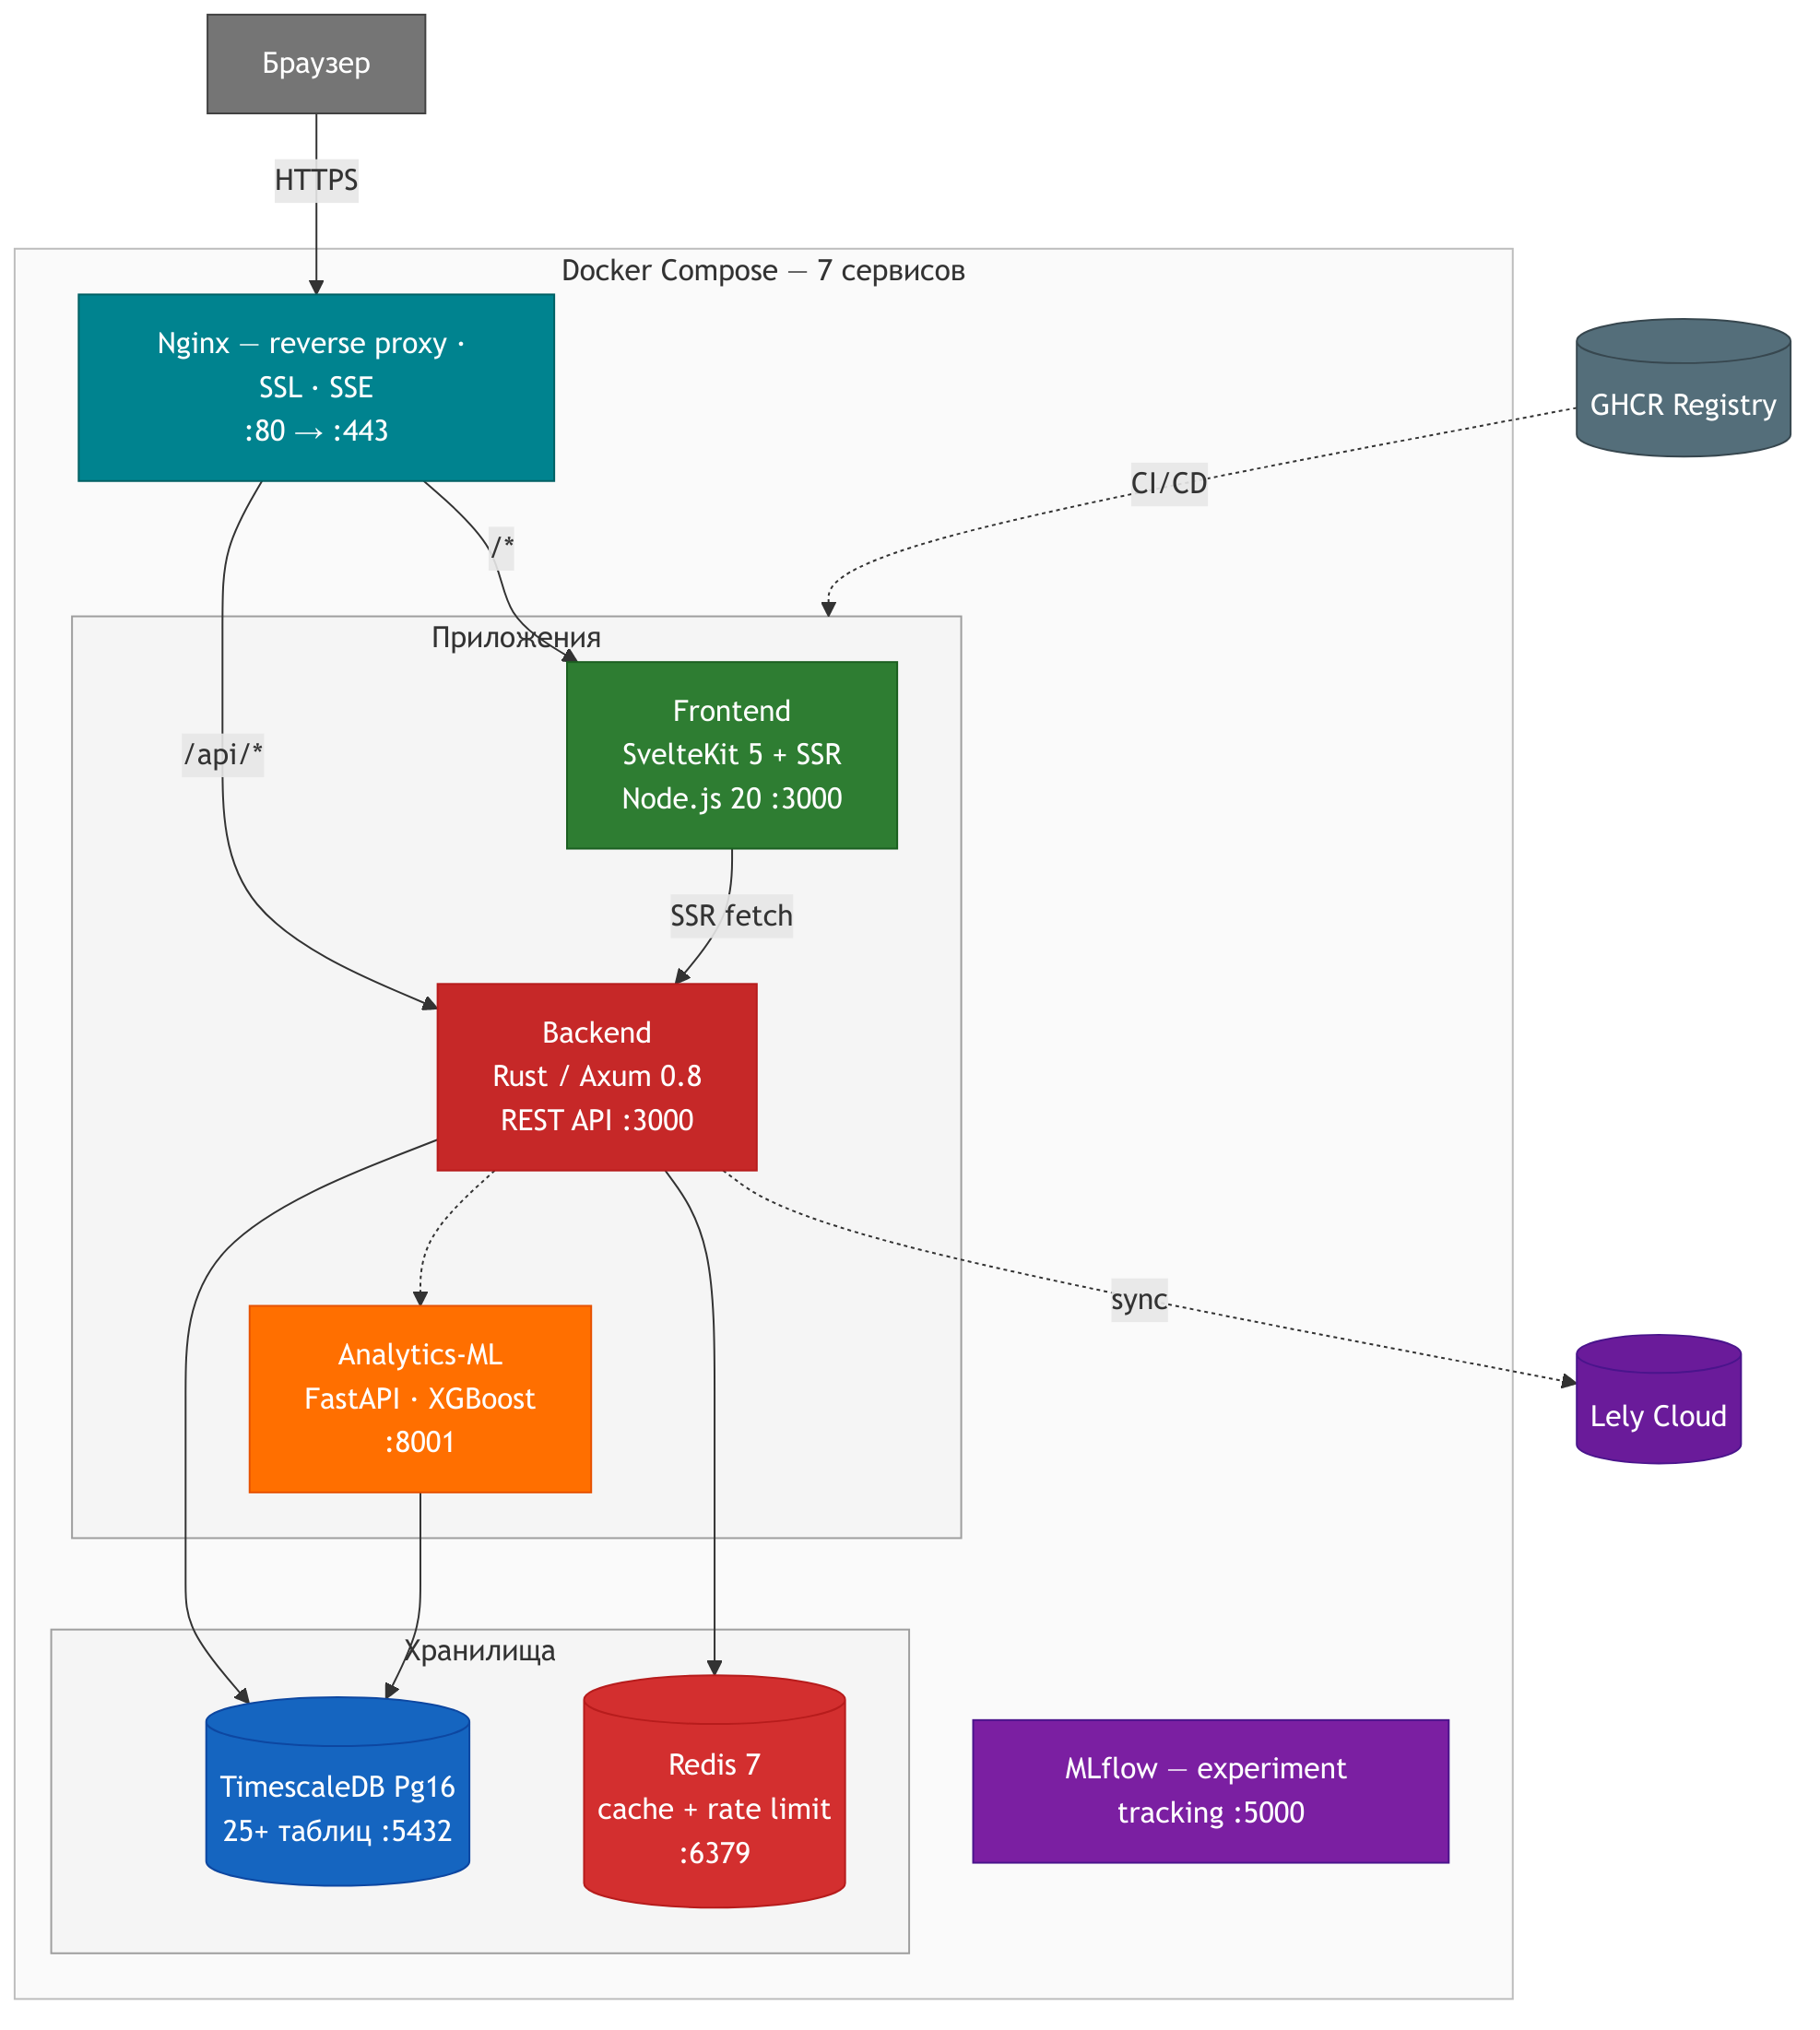
\includegraphics[width=0.95\textwidth,height=0.85\textheight,keepaspectratio]{container.png}
  \caption{Архитектура информационной системы}
  \label{arch}
\end{figure}

Архитектурные решения обоснованы несколькими соображениями. Разделение ответственности обеспечивает чёткое разграничение: backend отвечает за бизнес-логику, frontend --- за пользовательский интерфейс, analytics-ml --- за модели машинного обучения. Независимое масштабирование позволяет запускать несколько экземпляров backend за балансировщиком нагрузки без изменения остальных компонентов. Технологическая гетерогенность даёт возможность использовать наиболее подходящий стек для каждого компонента (Rust для серверной части, Svelte для клиента, Python для ML). Изоляция сбоев, обеспечиваемая контейнерной изоляцией Docker, гарантирует, что сбой одного компонента не приводит к отказу всей системы.

\subsection{Модель данных}

Архитектура системы определяет структуру хранилища данных, к описанию которой мы переходим. База данных PostgreSQL содержит более 35 таблиц, обеспечивающих хранение всех сущностей предметной области. Перечень таблиц с назначением приведён в приложении~\ref{app-db}, полная ER-модель --- в приложении~\ref{app-er}. На рисунке~\ref{er} представлена модель данных системы.

\begin{figure}
  \centering
  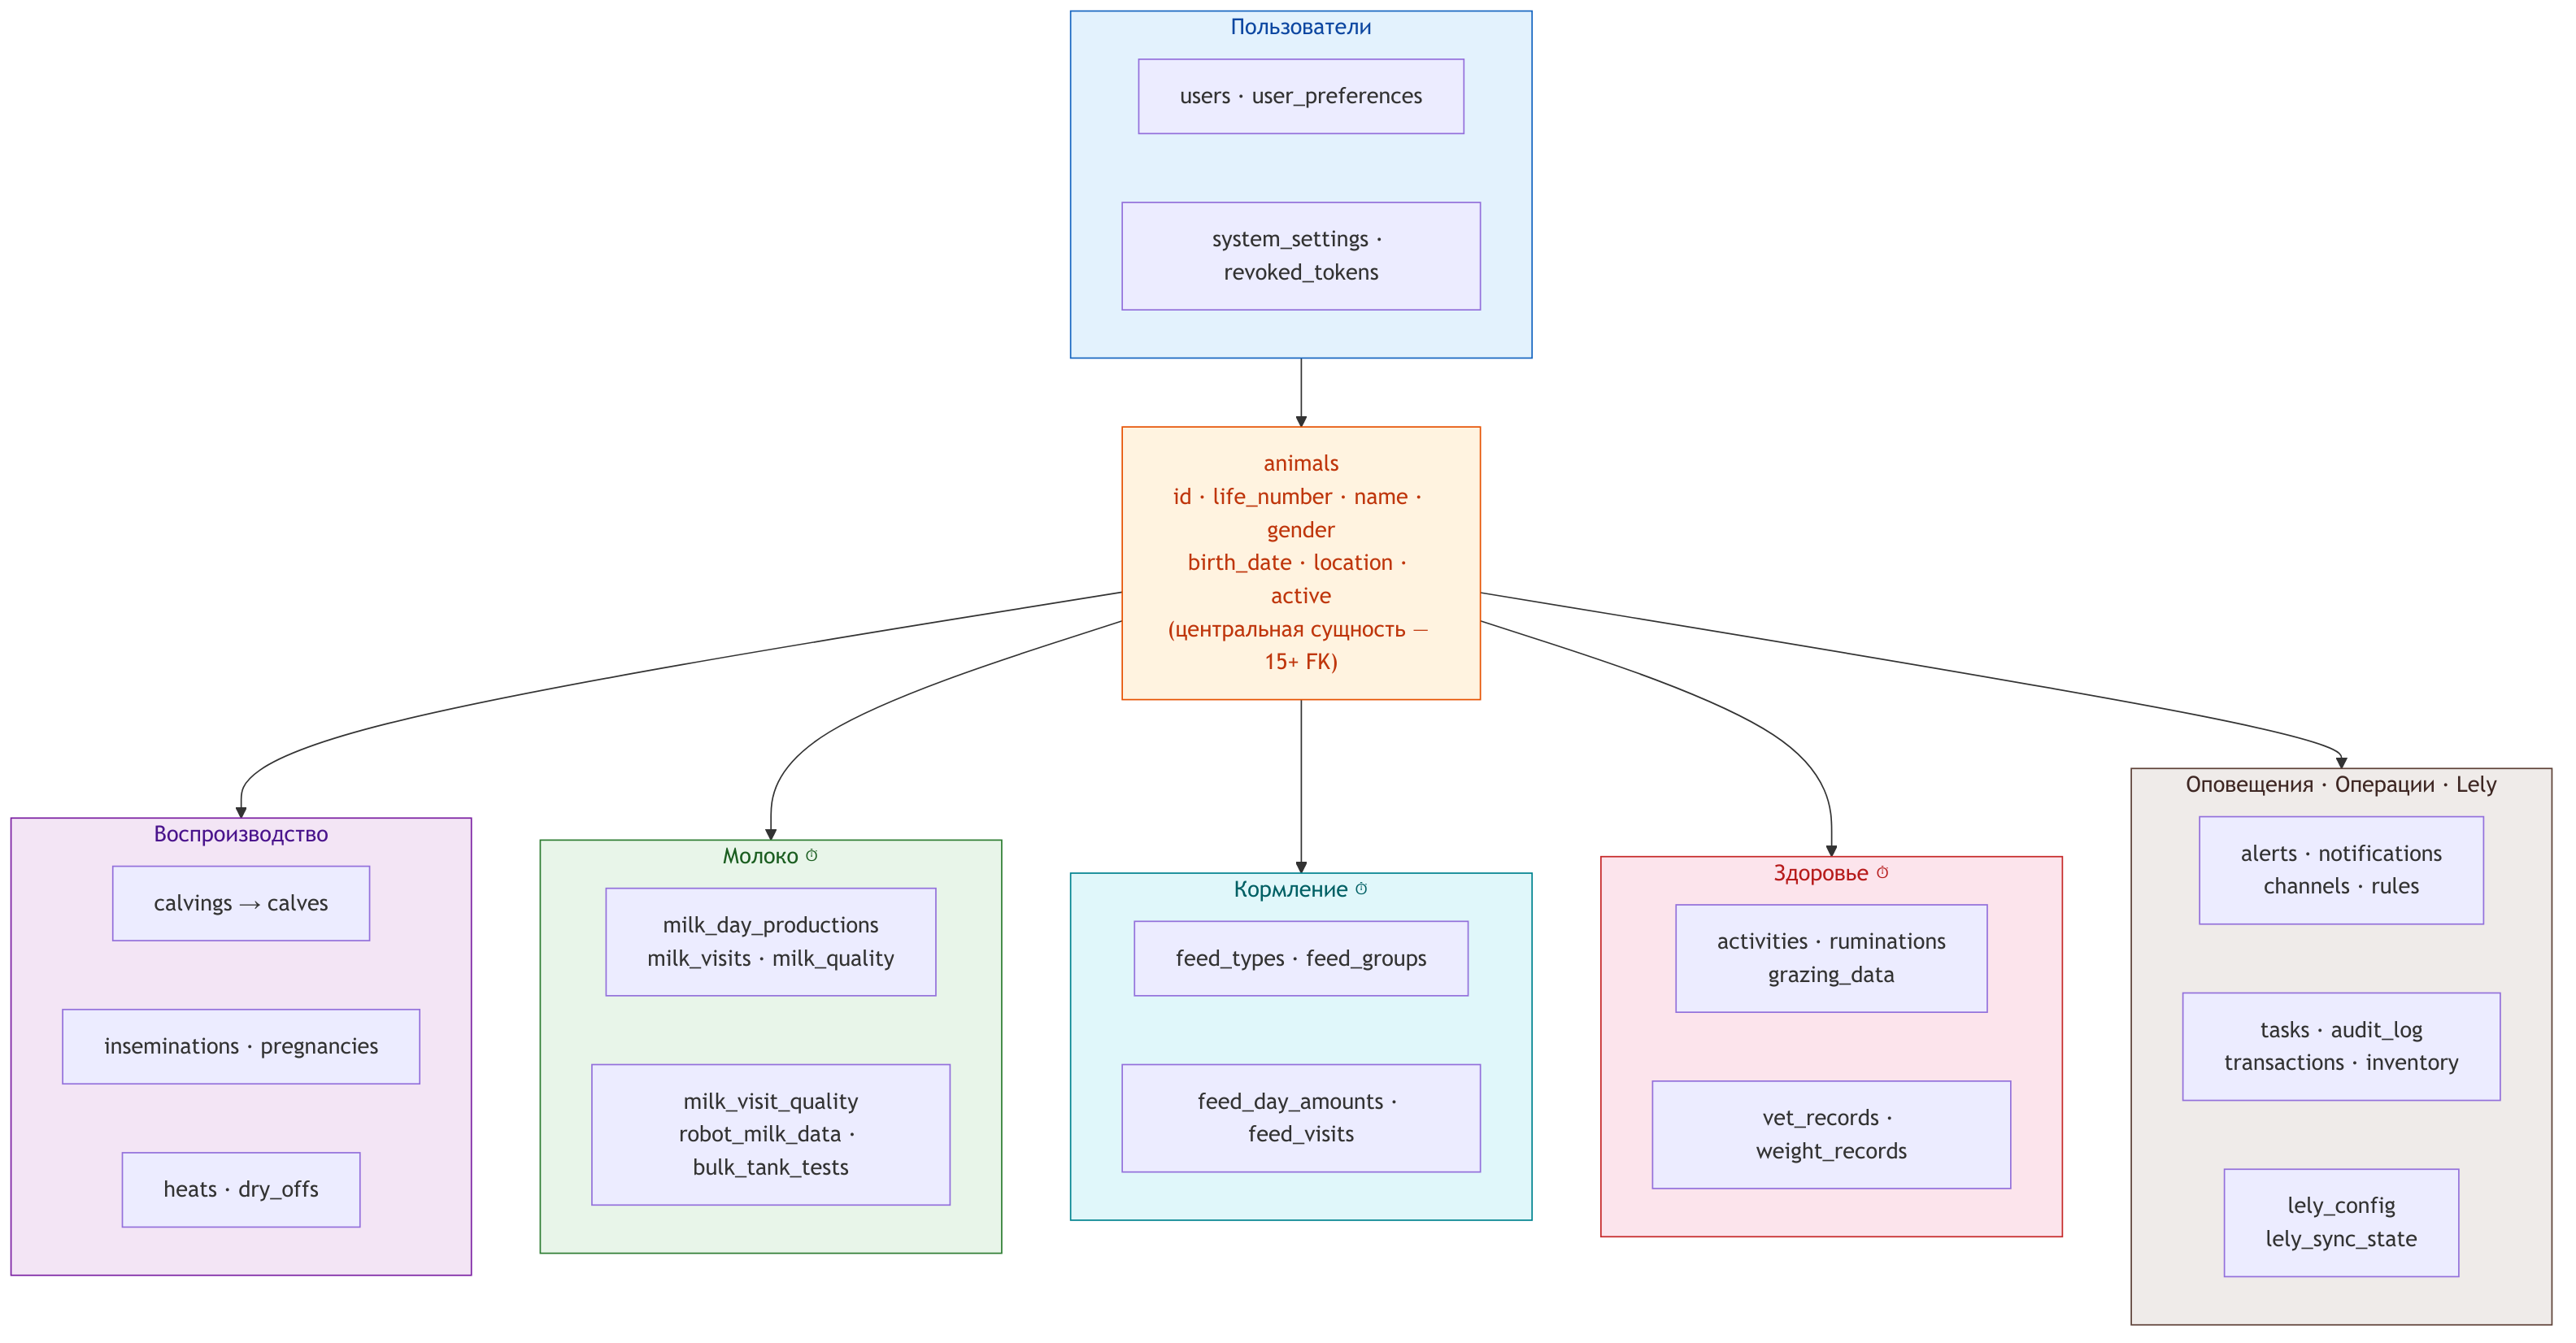
\includegraphics[width=0.95\textwidth,height=0.85\textheight,keepaspectratio]{database-model.png}
  \caption{Модель данных информационной системы}
  \label{er}
\end{figure}

Основные таблицы базы данных и их назначение:

\textbf{users} --- пользователи системы. Содержит имя пользователя, хеш пароля (bcrypt), роль (admin/user), флаг обязательной смены пароля и дату создания. Пароли хранятся в виде хешей с использованием алгоритма bcrypt с автоматической генерацией соли, что исключает утечку паролей при компрометации базы данных.

\textbf{animals} --- реестр животных. Содержит уникальный идентификатор, инвентарный номер (life\_number), кличку, пол, дату рождения, породу, местоположение, статус активности и множество других полей. Поддерживается флаг \texttt{active} для деактивации животных без удаления записей, что обеспечивает сохранение истории.

\textbf{milk\_day\_productions} --- суточные надои. Привязаны к животному и дате. Содержат объём молока (кг), жир (\%), белок (\%), лактозу (\%), количество соматических клеток (\acrshort{scc}), энергию (MJ) и жирово-белковое соотношение (\acrshort{fpr}). Композитный индекс (animal\_id, date) обеспечивает быстрый поиск надоев за период.

\textbf{milk\_visits} --- визиты на доение. Содержат информацию о каждом доении: время начала и окончания, объём молока, скорость доения (кг/мин), данные по четвертям вымени (объём, время, процент выдаивания), флаг успешности доения и идентификатор робота.

\textbf{milk\_quality} --- результаты лабораторных анализов молока. Включает количество соматических клеток (\acrshort{scc}), жир, белок, лактозу, мочевину, бактерии.

\textbf{calvings, calves, inseminations, pregnancies, heats, dry\_offs} --- данные о воспроизводстве. Каждая таблица связана с животным через внешний ключ. Поддерживается полная история всех событий воспроизводства, включая дату события, результат и примечания.

\textbf{feed\_types, feed\_groups, feed\_day\_amounts, feed\_visits} --- данные о кормлении. Типы кормов описывают рационы с указанием стоимости и единиц измерения, группы --- привязку кормов к группам животных, дневные объёмы --- плановое и фактическое потребление, визиты --- отдельные посещения кормостанции с временем и объёмом.

\textbf{activities, ruminations, grazing\_data} --- данные фитнес-мониторинга и пастьбы. Активность измеряется в шагах за период, жвачка --- в минутах жевания за период.

\textbf{alerts} --- система оповещений. Оповещения создаются автоматически на основе настраиваемых пороговых значений. Каждое оповещение содержит категорию (milk, health, reproduction, feed, equipment), степень важности (high, medium, low), статус (active, acknowledged, resolved), идентификатор животного и текстовое описание.

\textbf{lely\_sync\_state} --- состояние синхронизации с Lely. Хранит дату последней успешной синхронизации для каждого типа данных, что позволяет инкрементально обновлять информацию и минимизировать объём данных при каждой синхронизации.

\textbf{lely\_config} --- конфигурация интеграции с Lely. Хранит URL API, зашифрованные логин и пароль, ключ фермы и настройки синхронизации. Учётные данные шифруются с использованием AES-256-GCM~\cite{AES-GCM}.

Для эффективной работы с временными рядами (надои, активность, жвачка) используется расширение TimescaleDB~\cite{TimescaleDB}. Таблицы с временными рядами преобразованы в гипертаблицы с автоматической партицировкой по времени (по умолчанию --- 7 дней на чанк), что ускоряет запросы за определённый период, так как сканируются только релевантные чанки. Непрерывные агрегаты (continuous aggregates) обеспечивают предвычисление суточных и часовых агрегатов, обновляемых в фоновом режиме.

Индексация включает уникальные ограничения (инвентарный номер животного), композитные индексы (животное + дата) и частичные индексы (только активные животные). Расширение pg\_trgm~\cite{PgTrgm} обеспечивает полнотекстовый поиск по кличкам животных с использованием триграммного сходства.

\subsection{Серверная часть (Backend)}

Спроектированная модель данных служит основой для серверной части, обеспечивающей бизнес-логику и API для клиентского приложения. Серверная часть реализована на языке Rust с использованием фреймворка Axum. Архитектура следует паттерну разделения на слои: HTTP-обработчики (handlers), сервисы бизнес-логики (services), модели данных (models) и промежуточное программное обеспечение (middleware). На рисунке~\ref{backend-arch} представлена архитектура серверной части.

\begin{figure}
  \centering
  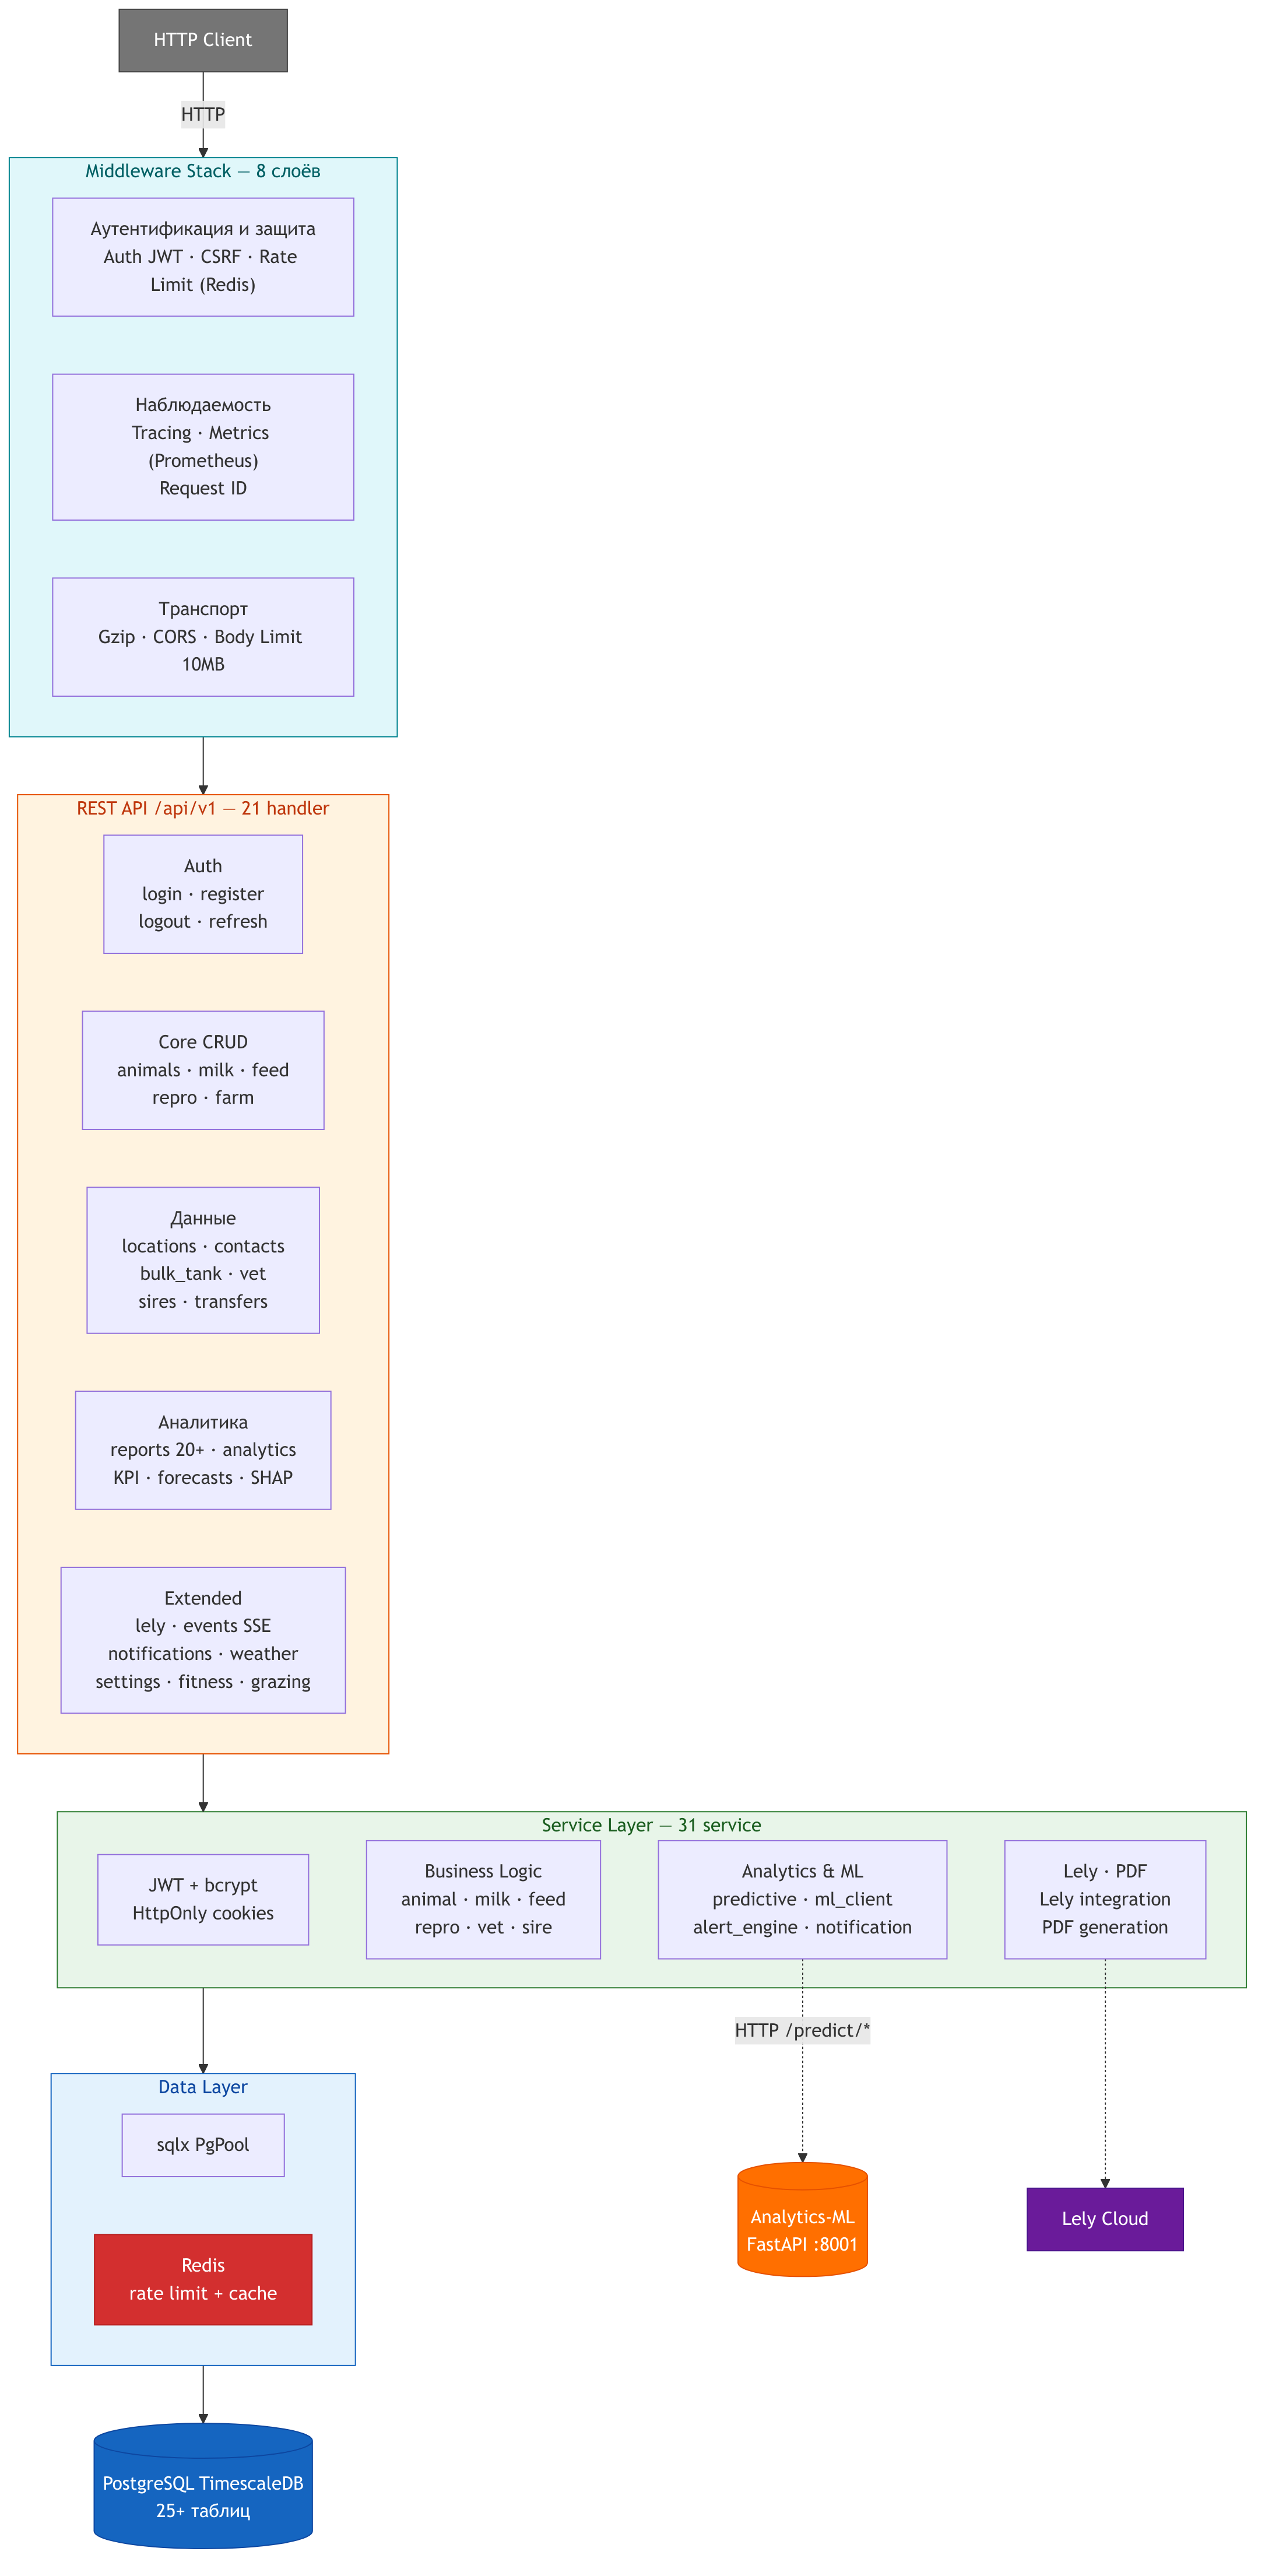
\includegraphics[width=0.95\textwidth,height=0.85\textheight,keepaspectratio]{backend-components.png}
  \caption{Архитектура серверной части}
  \label{backend-arch}
\end{figure}

\subsubsection{Маршрутизация и обработка запросов}

Все API-эндпоинты доступны по префиксу \texttt{/api/v1/}. Маршруты сгруппированы по доменным областям: животные, надои, воспроизводство, кормление, фитнес, отчёты, аналитика, настройки и другие. Общее количество обработчиков --- более 25 модулей. Примеры запросов и ответов приведены в приложении~\ref{app-api}.

Документация API генерируется автоматически с помощью библиотеки utoipa~\cite{utoipa} на основе аннотаций в коде и доступна через Swagger UI по адресу \texttt{/api/v1/docs}. Аннотации включают описание эндпоинтов, типы запросов и ответов, коды ошибок.

\subsubsection{Аутентификация и авторизация}

Аутентификация основана на \acrshort{jwt}~\cite{JWT} (JSON Web Token) с алгоритмом HS256. При входе в систему сервер выдаёт два токена: короткоживущий access token (15 минут) и долгоживущий refresh token (7 дней) для обновления access token без повторного ввода пароля.

Токены хранятся в HttpOnly, SameSite=Strict cookie, что предотвращает доступ к ним из JavaScript и обеспечивает защиту от CSRF-атак~\cite{OWASP-CSRF}. Отзыв токенов реализован через таблицу \texttt{revoked\_tokens}, хранящую JTI отозванных токенов. Просроченные записи удаляются ежечасно фоновым заданием.

Авторизация реализована через три уровня доступа, соответствующих типам Axum-экстракторов. Уровень \textbf{Claims} допускает любого аутентифицированного пользователя с валидным access token. Уровень \textbf{ClaimsAllowMustChange} допускает состояние обязательной смены пароля. Уровень \textbf{AdminGuard} ограничивает доступ пользователями с ролью \texttt{admin}.

\subsubsection{Промежуточное программное обеспечение (Middleware)}

Стек middleware обеспечивает безопасность, наблюдаемость и ограничение нагрузки. \textbf{CORS} настраивает кросс-доменный доступ~\cite{CORS} с конфигурируемыми источниками. \textbf{CSRF-защита} проверяет заголовок Origin для изменяющих состояние запросов. \textbf{Rate Limiting} ограничивает частоту запросов по IP-адресу (100 запросов за 60 секунд) с использованием Redis. \textbf{Gzip-сжатие} уменьшает объём передаваемых данных. \textbf{Логирование} обеспечивает трассировку HTTP-запросов через tracing с поддержкой структурированных логов в JSON-формате. \textbf{Метрики Prometheus} включают счётчики \texttt{http\_requests\_total} и гистограммы \texttt{http\_request\_duration\_seconds} с нормализацией маршрутов.

\subsubsection{Интеграция с Lely}

Модуль интеграции с Lely обеспечивает автоматическую двустороннюю синхронизацию данных с облачным API Lely Horizon. Синхронизация выполняется по настраиваемому таймеру (по умолчанию каждые 5 минут).

Архитектура модуля включает HTTP-клиент с аутентификацией по токену и автоматическим обновлением каждые 58 минут, а также повторными попытками с экспоненциальной задержкой. Планировщик синхронизации поддерживает параллельные задачи и инкрементальную синхронизацию по временным диапазонам (чанками по 7 дней). Маппинг данных использует кэш инвентарных номеров для разрешения Life Number Lely во внутренний идентификатор животного. Upsert-логика выполняет добавление или обновление записей через INSERT ON CONFLICT UPDATE. Учётные данные шифруются алгоритмом AES-256-GCM~\cite{AES-GCM}.

Синхронизируются 23 типа данных: животные, отёлы, осеменения, стельности, охоты, запуски, суточные надои, визиты на доение, качество молока, данные роботов, кормление, активности, жвачка, пастьба, быки-производители, переводы, кровные линии, типы и группы кормов, контакты, местоположения.

\subsection{Клиентское веб-приложение (Frontend)}

Серверный API, описанный выше, используется клиентским веб-приложением, обеспечивающим пользовательский интерфейс системы. Клиентское приложение реализовано на SvelteKit 2 с Svelte 5~\cite{Svelte5} и представляет собой одностраничное приложение (\acrshort{spa}) с серверным рендерингом (\acrshort{ssr}). На рисунке~\ref{frontend-arch} представлена архитектура клиентского приложения.

\begin{figure}
  \centering
  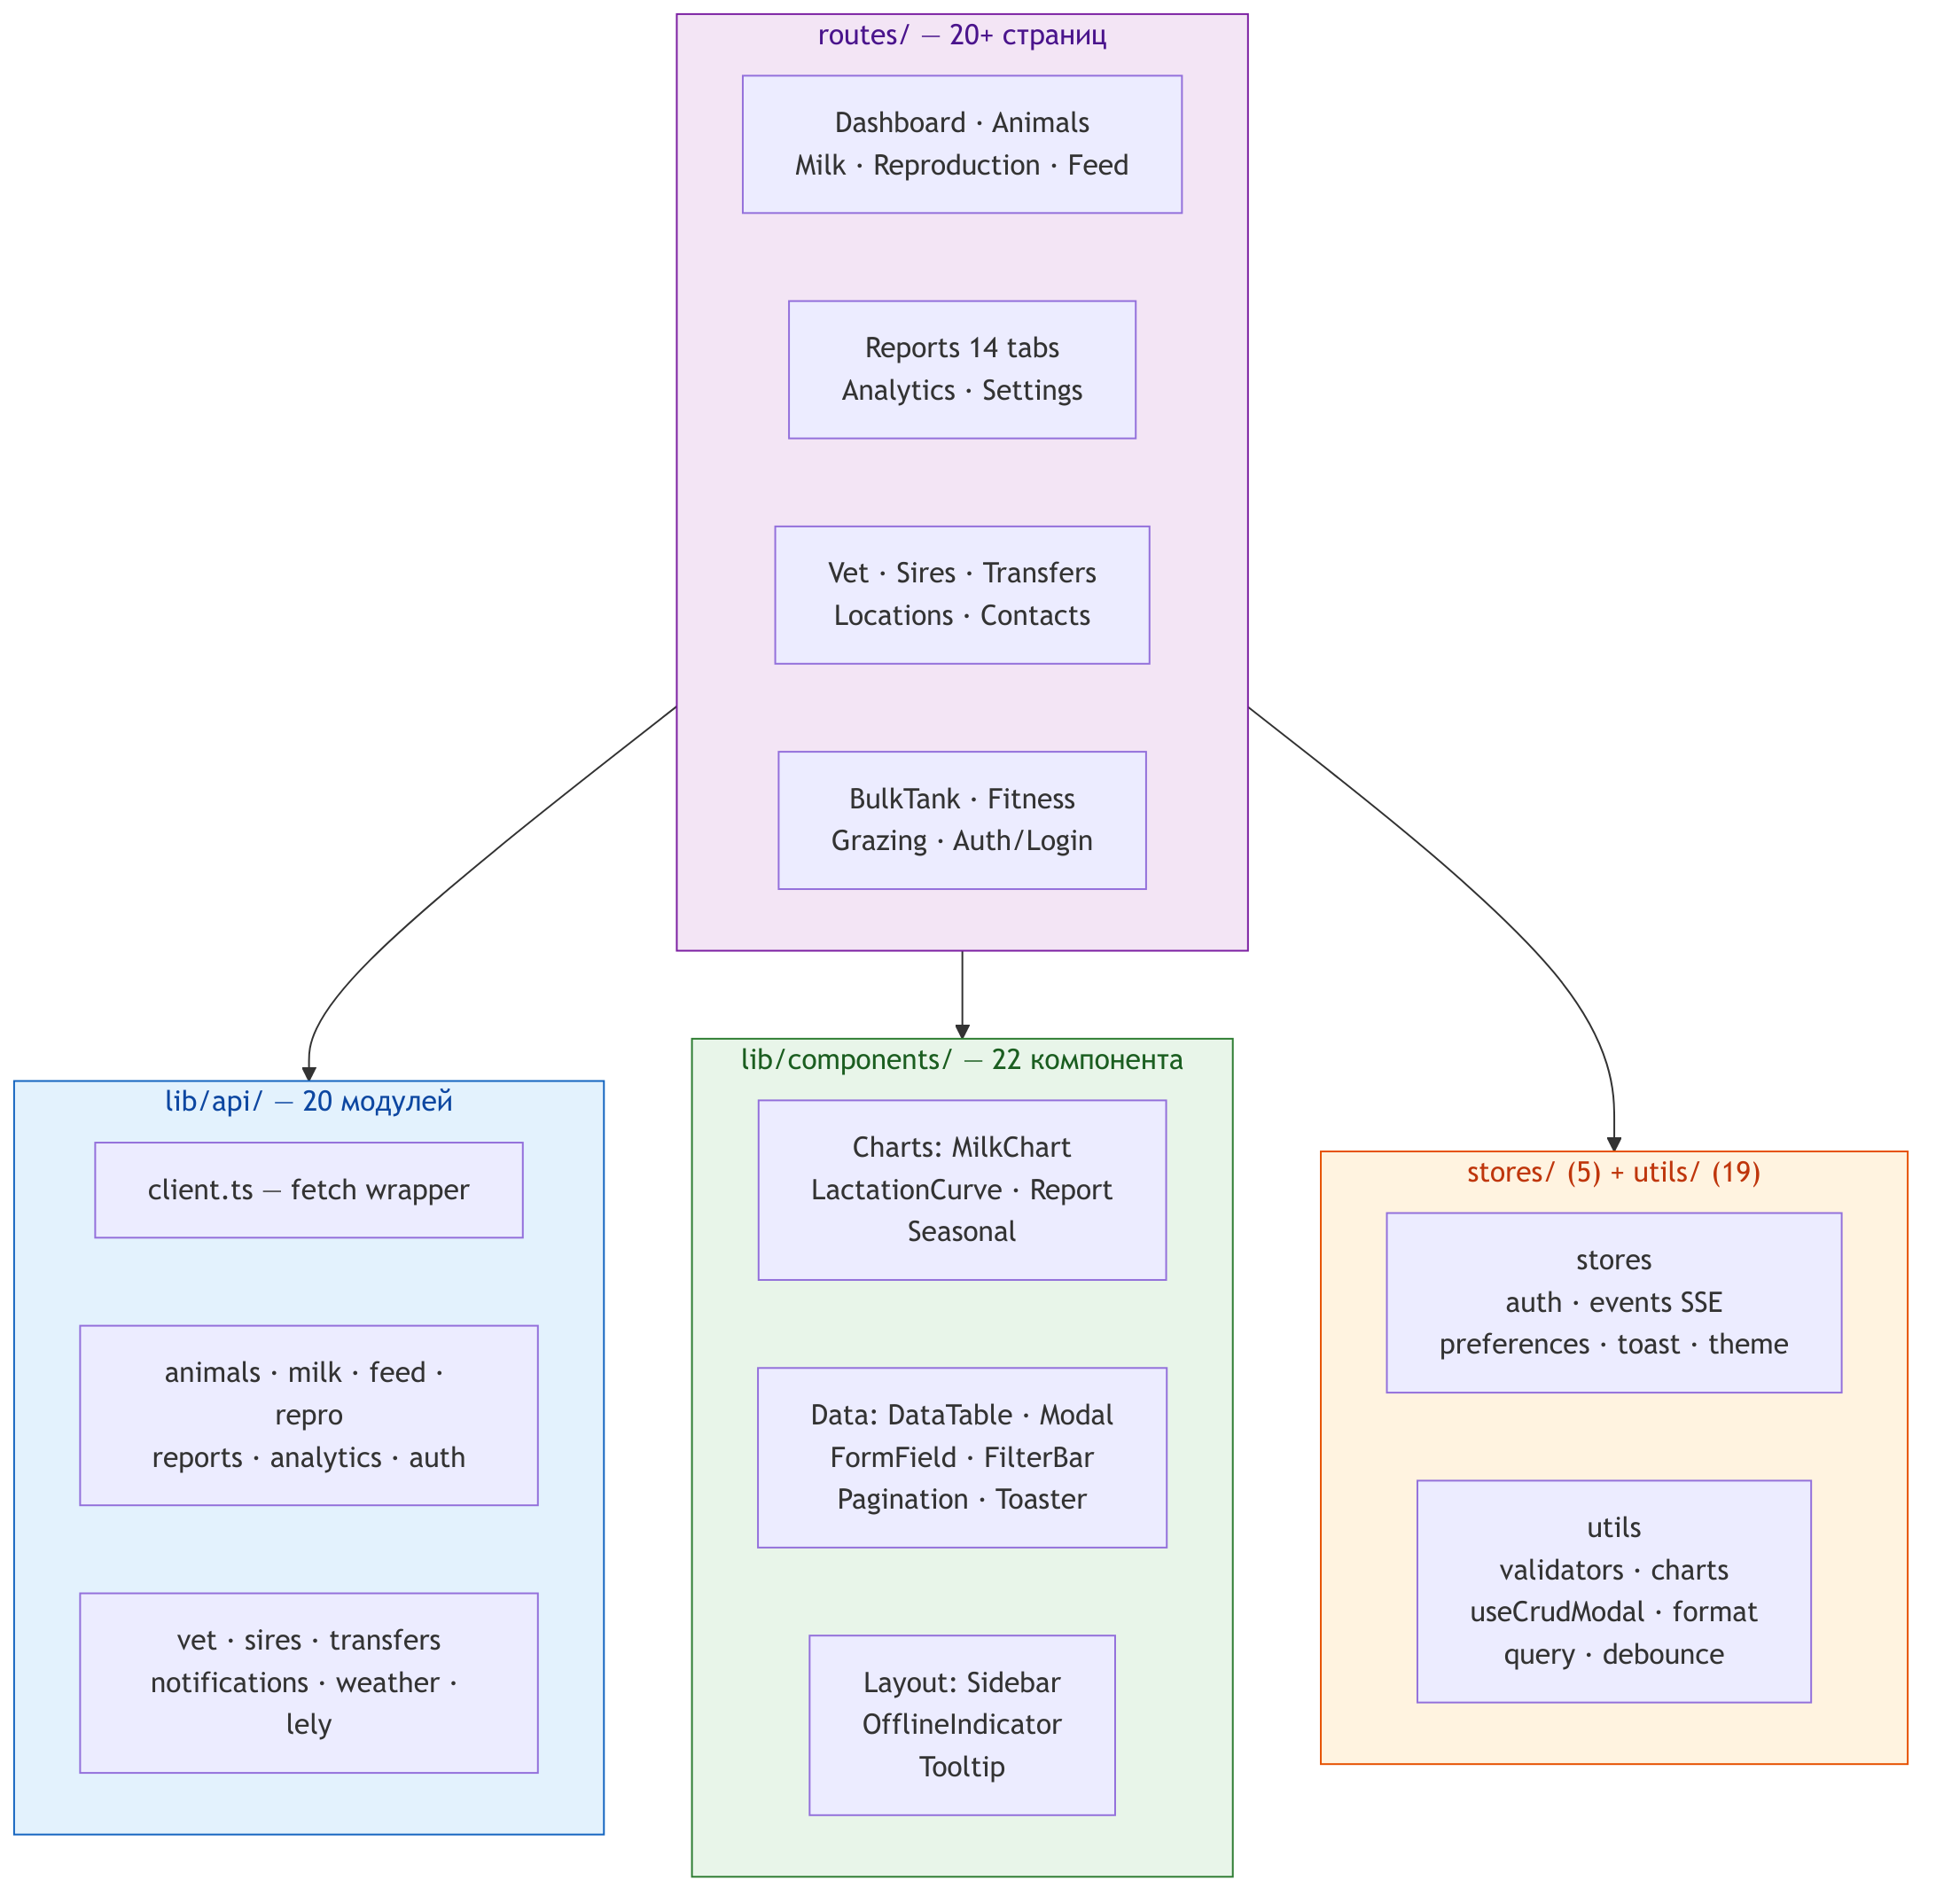
\includegraphics[width=0.95\textwidth,height=0.85\textheight,keepaspectratio]{frontend-structure.png}
  \caption{Архитектура клиентского веб-приложения}
  \label{frontend-arch}
\end{figure}

\subsubsection{Маршрутизация и навигация}

Приложение содержит более 24 страниц, сгруппированных по функциональным областям: дашборд, животные, надои, воспроизводство, кормление, фитнес, пастьба, отчёты, аналитика, настройки, контакты, местоположения, быки, переводы, запасы, оповещения, задачи, ветеринария, финансы, рентабельность, поиск.

Навигация реализована через боковую панель (Sidebar) с иконками из библиотеки Lucide и группировкой разделов. Адаптивная верстка на основе Tailwind CSS обеспечивает корректное отображение на мобильных устройствах: на экранах менее 768px боковая панель сворачивается в гамбургер-меню.

\subsubsection{Аутентификация на стороне клиента}

Серверный хук (hooks.server.ts) проверяет наличие \acrshort{jwt} в cookie при каждом запросе. Декодируется полезная нагрузка токена и проверяется срок действия. Неаутентифицированные пользователи перенаправляются на страницу входа, аутентифицированные --- не могут перейти на страницу входа.

Управление состоянием аутентификации реализовано через Svelte-стор (auth store), который инициализируется при загрузке приложения через endpoint refresh.

\subsubsection{API-клиент}

Клиент для взаимодействия с серверным API реализует автоматическое обновление токена: при получении ответа 401 выполняется попытка обновления access token через \texttt{/auth/refresh}; если refresh-токен также недействителен, пользователь разлогинивается и перенаправляется на страницу входа.

Для повышения надёжности реализован механизм повторных попыток: до 3 попыток с экспоненциальной задержкой (500 мс базовая задержка + случайный джиттер) для ответов с кодом 5xx. API-клиент разделён на 23 модуля по доменным областям.

\subsubsection{Компоненты пользовательского интерфейса}

Библиотека переиспользуемых компонентов включает DataTable --- таблицу данных с сортировкой по столбцам, серверной пагинацией и адаптивным отображением на мобильных устройствах; Modal и ConfirmDialog --- модальные окна для создания, редактирования и подтверждения действий; FormField --- компонент формы с поддержкой валидации и отображения ошибок; FilterBar --- панель фильтров с поддержкой текстового поиска, выпадающих списков и диапазонов дат; MilkChart, LactationCurveChart, ReportChart, SeasonalChart --- компоненты визуализации данных на основе Chart.js; Toaster --- уведомления с раскрываемыми подробностями и автоматическим скрытием.

Валидация форм реализована на основе Svelte 5 Runes --- реактивной системы состояния, позволяющей декларативно описывать правила валидации и отслеживать состояние формы (dirty, errors, touched).

\subsubsection{Генерация отчётов}

Система поддерживает генерацию отчётов более 17 типов, покрывающих все аспекты управления стадом. Каждый отчёт доступен в формате JSON для отображения в интерфейсе, а также поддерживает экспорт в CSV и PDF. Ключевые типы отчётов перечислены в таблице~\ref{reports}.

\begin{table}
  \caption{Основные типы отчётов системы}
  \begin{tabular}{|c|l|p{6cm}|}
    \hline
    \textbf{Код} & \textbf{Название} & \textbf{Описание} \\
    \hline
    R12 & Здоровье вымени & Рабочий список коров с отклонениями за 24 часа \\
    \hline
    R13 & Неудачные доения & Визиты с неуспешным доением \\
    \hline
    R16 & Обзор стада & Дневная производительность стада \\
    \hline
    R18 & Остаток корма & Невыданный корм по коровам \\
    \hline
    R20 & Надой по времени & Суточный надой с разбивкой по показателям \\
    \hline
    R23 & Анализ вымени & Расширенный анализ за 14 дней \\
    \hline
    R24 & Активность/жвачка & Здоровье, активность и жвачка \\
    \hline
    R31-34 & Календарь & Ожидаемые отёлы, запуски, охота, стельность \\
    \hline
    R41 & Эффективность & Эффективность корова-робот \\
    \hline
    R52 & Лактация & Кривые лактации по номерам \\
    \hline
    R56 & Робот & Производительность роботов \\
    \hline
    R70 & Корм по типам & Стоимость и объём кормов по типам \\
    \hline
    R72 & Корм на корову & Потребление корма на корову \\
    \hline
  \end{tabular}
  \label{reports}
\end{table}

\subsection{Модуль машинного обучения (Analytics-ML)}

Наряду с серверной частью и клиентским приложением, система включает модуль машинного обучения, отвечающий за предиктивную аналитику. Модуль реализован на Python с использованием FastAPI и предоставляет API для прогнозирования и обнаружения аномалий. На рисунке~\ref{ml-arch} представлена архитектура модуля машинного обучения.

\begin{figure}
  \centering
  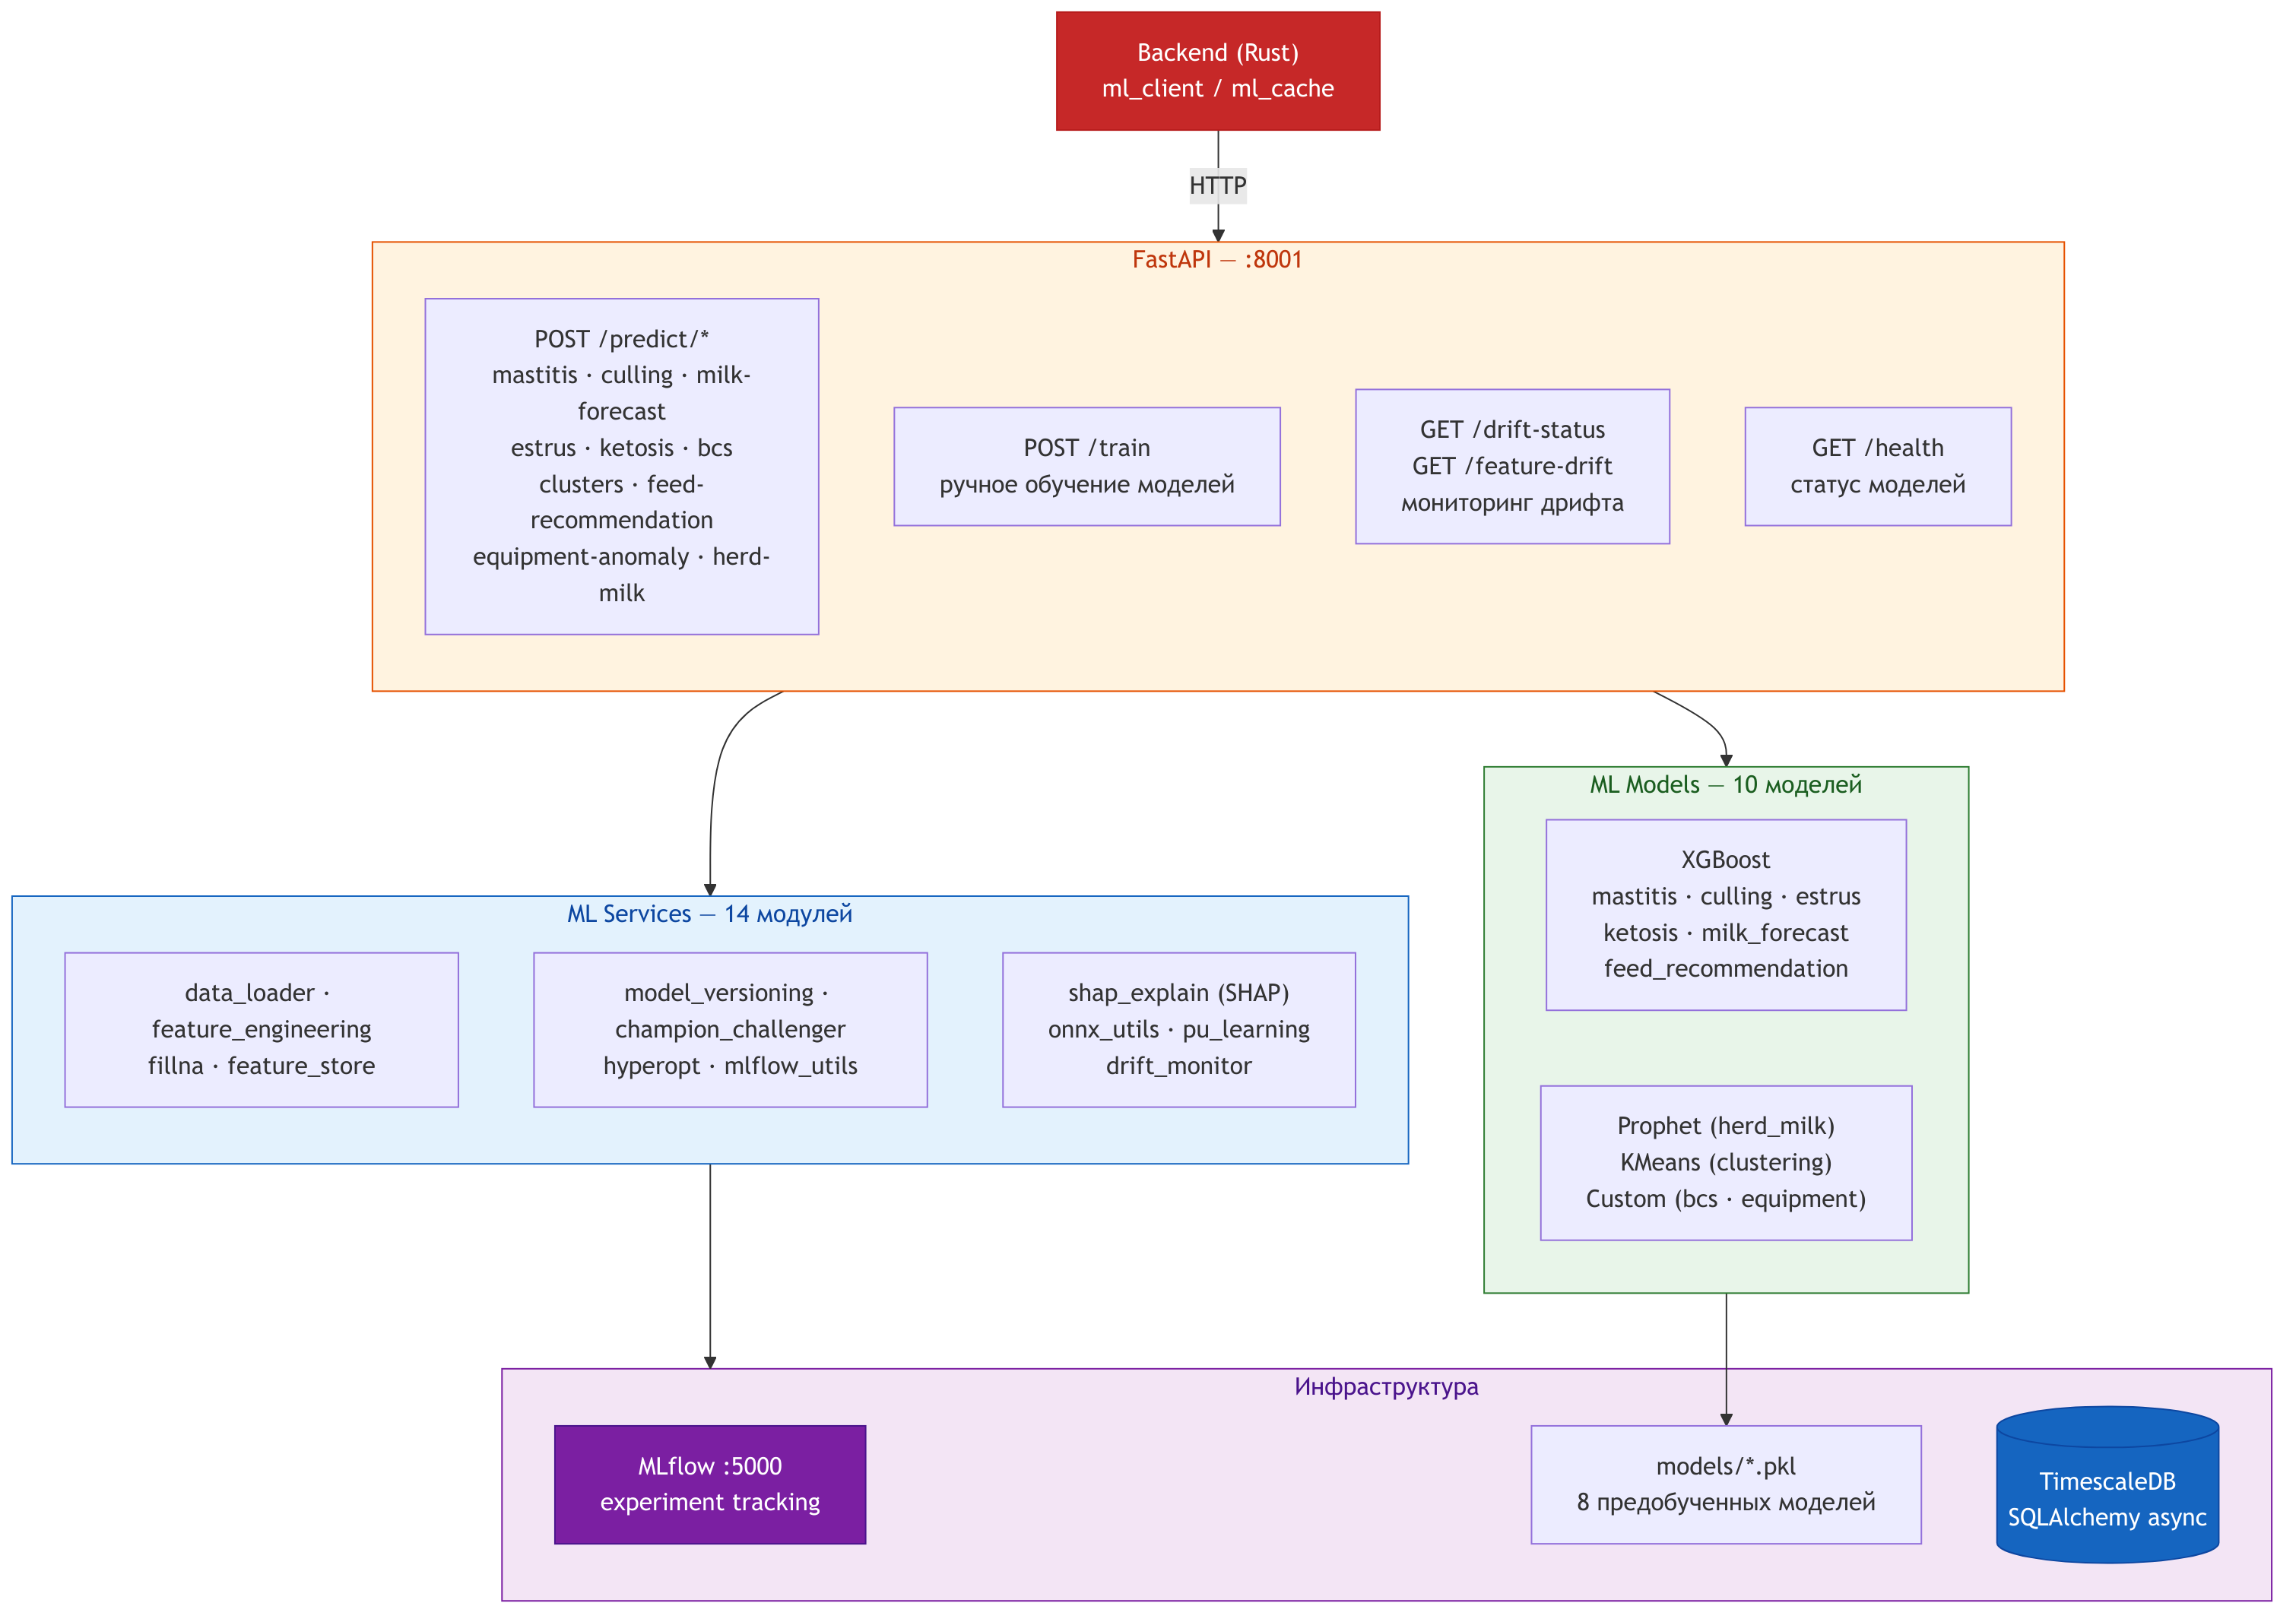
\includegraphics[width=0.95\textwidth,height=0.85\textheight,keepaspectratio]{analytics-ml.png}
  \caption{Архитектура модуля машинного обучения}
  \label{ml-arch}
\end{figure}

\subsubsection{Выбор алгоритмов}

Все задачи предиктивной аналитики в системе формулируются на табулярных данных, образованных агрегированными показателями животных (надои, активность, жвачка, SCC) за скользящие временные окна. Для таких данных методы градиентного бустинга показывают состояние-of-the-art результаты~\cite{XGBoost}, превосходя нейросетевые подходы на выборках умеренного размера (сотни---тысячи записей), характерных для одной фермы.

Система автоматически выбирает наилучший алгоритм градиентного бустинга среди трёх реализаций: XGBoost~\cite{XGBoost}, LightGBM~\cite{LightGBM} и CatBoost~\cite{CatBoost}. Выбор обусловлен различиями в подходах к построению деревьев: XGBoost использует уровень-wise рост, обеспечивая стабильность на сбалансированных данных; LightGBM применяет лист-wise рост с гистограммной оптимизацией, что ускоряет обучение на больших выборках; CatBoost использует ordered boosting, устойчивый к утечке целевой переменной (target leakage). Гипероптимизация Optuna проводит испытания равномерно по всем трём бэкендам и выбирает лучший по результатам кросс-валидации.

Для кластеризации стада используется алгоритм KMeans~\cite{KMeans}, либо HDBSCAN~\cite{HDBSCAN} при наличии кластеров произвольной формы; выбор производится автоматически по метрике силуэта. Для обнаружения аномалий оборудования применяется Isolation Forest~\cite{IsolationForest}, не требующий размеченных данных и устойчивый к высокой доле аномалий. Для прогнозирования на уровне стада используется Prophet~\cite{Prophet}, автоматически декомпозирующий временной ряд на тренд, сезонность и эффекты особых дней.

Разработано 11 моделей машинного обучения (таблица~\ref{mlmodels}).

\begin{table}
  \caption{Модели машинного обучения}
  \small
  \begin{tabularx}{\textwidth}{|p{3.2cm}|p{2.8cm}|l|X|}
    \hline
    \textbf{Модель} & \textbf{Алгоритм} & \textbf{Метрика} & \textbf{Назначение} \\
    \hline
    Прогноз надоев (корова) & XGBoost, квантильная регрессия & MAE & Дневной надой с q10/q90 интервалами \\
    \hline
    Прогноз надоев (стадо) & Prophet & --- & Тренд надоя стада с сезонностью \\
    \hline
    Риск мастита & XGBoost / LightGBM / CatBoost & ROC-AUC & Вероятность мастита \\
    \hline
    Предупреждение кетоза & XGBoost / LightGBM / CatBoost & ROC-AUC & Риск метаболического нарушения \\
    \hline
    Обнаружение охоты & XGBoost / LightGBM / CatBoost & ROC-AUC & Состояние (в охоте / нет) \\
    \hline
    Риск выбраковки & XGBoost / LightGBM / CatBoost & $R^2$ & Дни до выбраковки \\
    \hline
    Оценка BCS & XGBoost / LightGBM / CatBoost & MAE & Упитанность (1,0--5,0) \\
    \hline
    Кластеризация стада & KMeans / HDBSCAN & Silhouette & Сегментация стада \\
    \hline
    Аномалии оборудования & Isolation Forest & Доля аномалий & Аномалии работы роботов \\
    \hline
    Рекомендации по корму & XGBoost / LightGBM / CatBoost & MAE & Объём корма \\
    \hline
    Комплексное здоровье & MultiOutput\newline Classifier & ROC-AUC & Мастит + кетоз + охота совместно \\
    \hline
  \end{tabularx}
  \label{mlmodels}
\end{table}

\subsubsection{Обоснование выбора метрик}

Для задач классификации (мастит, кетоз, охота) выбрана метрика ROC-AUC (Area Under the Receiver Operating Characteristic Curve), поскольку она инвариантна к порогу принятия решения и соотношению классов. Это критично для veterinary-задач, где положительный класс составляет менее 5~процентов наблюдений: метрики accuracy и precision при таком дисбалансе неинформативны. ROC-AUC оценивает способность модели ранжировать наблюдения по степени риска, что соответствует прикладной задаче --- выделить животных с наибольшей вероятностью заболевания для приоритетного осмотра.

Для задач регрессии (прогноз надоев, рекомендации по корму, BCS) выбрана MAE (Mean Absolute Error), а не MSE/ RMSE. Обоснование: MAE менее чувствительна к выбросам, которые характерны для данных доильных роботов (пропущенное доение, сбой датчика). Кроме того, MAE измеряется в тех же единицах, что и целевая переменная (кг молока, кг корма), что упрощает интерпретацию результатов фермером.

Для кластеризации выбрана метрика силуэта, оценивающая компактность и разделимость кластеров без необходимости внешних меток.

Оценка всех моделей производится методом $k$-кратной кросс-валидации, где число фолдов адаптируется к объёму данных: $k = \min(5, \max(2, N / n))$, где $N$ --- количество наблюдений, $n$ --- минимальный размер фолда.

\subsubsection{Формирование обучающих меток}

Особенностью задач обнаружения заболеваний является отсутствие надёжных размеченных данных: ветеринарные записи неполны, а диагноз часто ставится с задержкой. Для решения этой проблемы применён подход обучения на положительных и неразмеченных данных (PU-learning)~\cite{PULearning}.

Метка <<мастит>> формируется на основе комбинации клинически обоснованных правил: SCC~>~300\,000 клеток/мл; либо SCC~>~200\,000 с трендом роста~>~1,5; либо SCC~>~150\,000 при повышенной электропроводности~>~55 мСм/см; либо отклонение надоя~>~15~процентов при SCC~>~100\,000. Аналогичные правила на основе FPR и жвачки используются для кетоза, а на основе соотношения активности и жвачки --- для охоты.

При наличии подтверждённых ветеринарных диагнозов они замещают эвристические метки с увеличением веса наблюдения в 3 раза, что позволяет модели постепенно переходить от semi-supervised к fully-supervised режиму по мере накопления данных.

\subsubsection{Прогноз надоев с доверительными интервалами}

Для прогнозирования надоев на корову обучаются три модели квантильной регрессии: для медианы (q50), нижней границы (q10) и верхней границы (q90). Объективная функция Quantile Loss для квантиля $\alpha$:

$$L_\alpha(y, \hat{y}) = \begin{cases} \alpha \cdot (y - \hat{y}), & \text{если } y \geq \hat{y} \\ (1 - \alpha) \cdot (\hat{y} - y), & \text{если } y < \hat{y} \end{cases}$$

где $y$ --- фактическое значение, $\hat{y}$ --- прогноз. Интервал q10--q90 содержит 80~процентов распределения прогнозов, позволяя фермеру количественно оценивать неопределённость.

\subsubsection{Инженерия признаков}

Для каждой модели формируется расширенный набор признаков на основе данных из PostgreSQL с использованием LATERAL JOIN для вычисления скользящих агрегатов. Признаки включают:

\begin{enumerate}
    \item лаговые --- значения целевого показателя за предыдущие 1, 7, 14, 30 дней;
    \item скользящие статистики --- среднее, стандартное отклонение, коэффициент вариации за окна 7, 14, 30 дней;
    \item трендовые --- отношение recent/baseline, наклон линейной регрессии за 7 и 14 дней;
    \item производные --- FPR, соотношение надой/корм, соотношение активность/жвачка;
    \item физиологические --- DIM, номер лактации, возраст;
    \item метеорологические --- температура, влажность, индекс температурно-влажностного стресса (THI);
    \item исторические --- количество ветеринарных обработок за 180 дней, дней с последней обработки;
    \item временные ряды --- энтропия, автокорреляция на лаге 1 и 7, сила тренда и сезонности.
\end{enumerate}

Для модели прогноза надоев дополнительно вычисляются TSFRESH-подобные признаки: приближённая энтропия, коэффициент эксцесса, максимальная просадка (drawdown), сила сезонности по STL-декомпозиции. Эти признаки позволяют модели различать стабильных и нестабильных коров.

Обработка пропущенных значений выполняется медианой по стаду, вычисленной на этапе обучения и сохраняемой вместе с моделью для обеспечения консистентности при прогнозировании. Дополнительно выполняется отбор признаков с помощью RandomForest importance: отбираются признаки с важностью выше медианной.

\subsubsection{MLOps: оптимизация, мониторинг дрейфа и управление моделями}

Оптимизация гиперпараметров осуществляется библиотекой Optuna~\cite{Optuna} с TPE-сэмплером (Tree-structured Parzen Estimator) в 8-мерном пространстве (learning\_rate, max\_depth, n\_estimators, min\_child\_weight, subsample, colsample\_bytree, reg\_alpha, reg\_lambda). Каждый испытание оценивается кросс-валидацией; по умолчанию выполняется 30 испытаний с таймаутом 120 секунд.

Мониторинг дрейфа реализован тремя методами. \textbf{Prediction drift} --- Z-тест: если $z = |\bar{x}_{\text{recent}} - \bar{x}_{\text{baseline}}| / \sigma_{\text{baseline}} > 2{,}0$, фиксируется сдвиг распределения прогнозов. \textbf{Feature drift} --- для каждого признака вычисляется Z-тест и критерий Колмогорова--Смирнова; дрейф фиксируется при $z > 2{,}5$ или $p_{\text{KS}} < 0{,}05$. \textbf{MMD-drift} --- Maximum Mean Discrepancy с RBF-ядром, оценивающий расстояние между распределениями в пространстве признаков; порог MMD~>~0{,}1.

При обнаружении дрейфа модель помечается для скорого переобучения, которое выполняется через APScheduler с настраиваемым расписанием (по умолчанию еженедельно).

Для управления моделями реализован подход <<чемпион--претендент>>: переобученная модель (претендент) сравнивается с текущей (чемпионом) на тех же данных; модель повышается только при улучшении метрики более чем на 1~процент. Это предотвращает деградацию при переобучении на зашумлённых данных.

Объяснимость прогнозов реализована через SHAP~\cite{SHAP} с использованием TreeExplainer для древовидных моделей. Отслеживание экспериментов осуществляется через MLflow~\cite{MLflow}. Для ускорения инференса модели экспортируются в формат ONNX.

\subsection{Предиктивная аналитика в серверной части}

Модуль машинного обучения на Python обеспечивает высокую точность прогнозов, однако его доступность зависит от состояния отдельного сервиса: при отказе или перезапуске analytics-ml предиктивная аналитика становится недоступна. Для обеспечения отказоустойчивости серверная часть содержит собственные алгоритмы аналитики, реализованные на Rust. Эти алгоритмы работают внутри процесса backend и не зависят от внешних сервисов, что гарантирует доступность базовой аналитики в любой момент.

\textbf{Метод Хольта--Винтерса}~\cite{HoltWinters} --- тройное экспоненциальное сглаживание для прогнозирования временных рядов надоев. Модель учитывает три компоненты: уровень (level), тренд (trend) и сезонность (seasonality). Рекуррентные формулы:

\begin{align}
l_t &= \alpha \cdot (y_t - s_{t-m}) + (1 - \alpha) \cdot (l_{t-1} + b_{t-1}) \\
b_t &= \beta \cdot (l_t - l_{t-1}) + (1 - \beta) \cdot b_{t-1} \\
s_t &= \gamma \cdot (y_t - l_t) + (1 - \gamma) \cdot s_{t-m}
\end{align}

где $l_t$ --- уровень, $b_t$ --- тренд, $s_t$ --- сезонная компонента, $m$ --- период сезонности (7 дней), $\alpha$, $\beta$, $\gamma$ --- параметры сглаживания. Прогноз на $h$ шагов вперёд:

$$\hat{y}_{t+h} = l_t + h \cdot b_t + s_{t+h-m}$$

Для обнаружения выбросов используется межквартильный размах (IQR): значение считается выбросом, если оно выходит за пределы $[Q_1 - 1.5 \cdot \text{IQR}, Q_3 + 1.5 \cdot \text{IQR}]$. Для обнаружения структурных сдвигов применяется t-критерий: если среднее последних 7 дней значимо отличается от среднего предыдущих 14 дней (p-value < 0.05), фиксируется структурный сдвиг.

\textbf{Кривая лактации Вуда}~\cite{LactationWood} --- лог-линейная модель, описывающая зависимость надоя от дня лактации:

$$y(t) = a \cdot t^b \cdot e^{-ct}$$

где $y(t)$ --- надой в день лактации $t$, $a$ --- масштабный коэффициент, определяющий начальный уровень надоя, $b$ --- параметр, контролирующий скорость нарастания до пика лактации, $c$ --- параметр, определяющий скорость спада после пика. Логарифмирование приводит к линейному виду:

$$\ln y(t) = \ln a + b \cdot \ln t - c \cdot t$$

Параметры оцениваются методом наименьших квадратов. Модель позволяет определять день пика лактации $t_{\max} = -b/c$ и сравнивать фактические надои с ожидаемыми для выявления отклонений.

\textbf{Индекс здоровья} --- составной показатель на основе z-оценок:

$$\text{Health Index} = -\frac{1}{n} \sum_{i=1}^{n} \left|z_i\right|$$

где $n = 4$ --- количество показателей, $z_i = (x_i - \mu_i) / \sigma_i$ --- стандартизованное отклонение $i$-го показателя (надои, \acrshort{scc}, активность, жвачка) от среднего $\mu_i$ и стандартного отклонения $\sigma_i$ по стаду. Индекс принимает значения от $-\infty$ до 0, где значения ниже $-2$ указывают на потенциальные проблемы со здоровьем.

\textbf{Оптимизатор запуска} --- определяет оптимальную дату сухостойного периода на основе прогноза лактации и планового отёла. Стандартный период запуска --- 60 дней до отёла. Оптимизатор корректирует дату с учётом текущего надоя.

\subsubsection{Сравнение моделей прогнозирования временных рядов}

Для повышения точности прогнозирования надоев реализована система автоматического сравнения 8 моделей прогнозирования. Исторические данные (90~дней) разбиваются на обучающую (80~процентов) и тестовую (20~процентов) выборки хронологически.

\textbf{MAPE} (Mean Absolute Percentage Error) --- основная метрика качества:

$$\text{MAPE} = \frac{100\%}{n} \sum_{i=1}^{n} \frac{|y_i - \hat{y}_i|}{|y_i|}$$

где $n$ --- количество наблюдений тестовой выборки, $y_i$ --- фактическое значение надоя, $\hat{y}_i$ --- прогнозное значение. MAPE выбран как основная метрика, поскольку она инвариантна к масштабу (надои разных коров могут отличаться в 2--3 раза).

\textbf{RMSE} (Root Mean Squared Error) дополняет MAPE, показывая типичное отклонение прогноза в абсолютных единицах (кг):

$$\text{RMSE} = \sqrt{\frac{1}{n} \sum_{i=1}^{n} (y_i - \hat{y}_i)^2}$$

В отличие от MAPE, RMSE усиливает штраф за крупные ошибки благодаря возведению в квадрат, что позволяет выявлять редкие, но значительные отклонения прогноза.

Лучшей моделью признаётся та, которая демонстрирует минимальный MAPE на тестовой выборке. Реализованы следующие модели:

\textbf{1. SES} (Simple Exponential Smoothing) --- простое экспоненциальное сглаживание:

$$\hat{y}_{t+1} = \alpha \cdot y_t + (1 - \alpha) \cdot \hat{y}_t$$

где $y_t$ --- фактическое значение надоя в момент $t$, $\hat{y}_t$ --- сглаженное значение, $\alpha \in (0, 1)$ --- параметр сглаживания, оптимизируемый перебором по сетке $\{0{,}05, 0{,}10, \ldots, 0{,}95\}$ с выбором минимального SSE (суммы квадратов ошибок).

\textbf{2. SMA} (Simple Moving Average) --- простое скользящее среднее с окном $w$.

\textbf{3. WMA} (Weighted Moving Average) --- взвешенное скользящее среднее с линейно возрастающими весами:

$$\hat{y}_{t+1} = \frac{\sum_{i=1}^{w} w_i \cdot y_{t-w+i}}{\sum_{i=1}^{w} w_i}$$

где $w$ --- размер окна (по умолчанию 7 дней), $w_i = i$ --- линейно возрастающий вес, придающий большую значимость недавним наблюдениям.

\textbf{4. Linear Regression} --- линейная регрессия по времени: $\hat{y}_t = a + b \cdot t$, где $a$ --- свободный член, $b$ --- наклон тренда, оцениваемые методом наименьших квадратов. Подходит для данных с выраженным линейным трендом, но не улавливает сезонность.

\textbf{5. Holt's Linear Method} --- двойное экспоненциальное сглаживание:

\begin{align}
l_t &= \alpha \cdot y_t + (1 - \alpha) \cdot (l_{t-1} + b_{t-1}) \\
b_t &= \beta \cdot (l_t - l_{t-1}) + (1 - \beta) \cdot b_{t-1}
\end{align}

где $l_t$ --- уровень, $b_t$ --- тренд, $\alpha$ и $\beta$ --- параметры сглаживания уровня и тренда соответственно. Прогноз: $\hat{y}_{t+h} = l_t + h \cdot b_t$.

\textbf{6. Holt--Winters} --- тройное экспоненциальное сглаживание с сезонной компонентой ($m = 7$ дней).

\textbf{7. Fourier Series} --- модель на основе рядов Фурье с линейным трендом:

$$\hat{y}_t = (a + b \cdot t) + \sum_{k=1}^{K} \left[ A_k \cos\!\left(\frac{2\pi t}{T_k}\right) + B_k \sin\!\left(\frac{2\pi t}{T_k}\right) \right]$$

где $a + b \cdot t$ --- линейный тренд, $K$ --- количество гармоник (по умолчанию 3), $T_k = 7/k$ --- период $k$-й гармоники в днях, $A_k$ и $B_k$ --- коэффициенты Фурье, оцениваемые методом наименьших квадратов. Базовый период 7 дней соответствует недельной сезонности надоев.

\textbf{8. ARIMA(0,1,1)} --- модель авторегрессии интегрированного скользящего среднего:

$$\Delta \hat{y}_t = \mu + \theta \cdot \varepsilon_{t-1}$$

где $\Delta \hat{y}_t = y_t - y_{t-1}$ --- первая разность надоя, $\mu$ --- средний дрифт (среднее суточное приращение), $\theta$ --- параметр скользящего среднего, $\varepsilon_{t-1}$ --- ошибка прогноза на предыдущем шаге. Данная спецификация эквивалентна экспоненциальному сглаживанию с дрифтом; для прогноза на $h \geq 2$ шагов вклад MA-члена равен нулю, и прогноз вырождается в прямую с наклоном $\mu$.

\subsubsection{Ансамблевый прогноз}

Для повышения робастности прогнозирования реализован ансамблевый метод, объединяющий три источника прогноза: ML-модель (XGBoost), нейросетевую модель (N-BEATS~\cite{NBEATS}) из ML-сервиса и лучшую статистическую модель (Rust). Нейросетевая модель N-BEATS использует архитектуру с базисными расширениями, способную улавливать нелинейные паттерны во временных рядах, недоступные статистическим методам.

Итоговый прогноз формируется как взвешенное среднее:

$$\hat{y}_t = w_{\text{ML}} \cdot \hat{y}_t^{\text{ML}} + w_{\text{NBEATS}} \cdot \hat{y}_t^{\text{NBEATS}} + w_{\text{Rust}} \cdot \hat{y}_t^{\text{Rust}}$$

Вес каждой модели определяется обратно пропорционально её MAPE: $w_i = (1 / (\text{MAPE}_i + 1)) / \sum_j (1 / (\text{MAPE}_j + 1))$. MAPE ML-модели и N-BEATS задаётся оценочно по результатам кросс-валидации (8 и 10~процентов соответственно), MAPE Rust-модели вычисляется динамически для каждого животного. Такое взвешивание придаёт больший вес более точным моделям, сохраняя при этом вклад каждой.

Если ML-сервис недоступен, система автоматически откатывается к прогнозу лучшей Rust-модели с весом 1,0, что гарантирует доступность прогноза при любом состоянии инфраструктуры.

\subsubsection{Объяснимость прогнозов (SHAP)}

Для обеспечения интерпретируемости прогнозов ML-сервис использует метод SHAP~\cite{SHAP}, основанный на теории кооперативных игр Шепли. Для каждого прогноза вычисляются SHAP-значения, показывающие вклад каждого признака в отклонение от базового значения модели:

$$\phi_i = \sum_{S \subseteq F \setminus \{i\}} \frac{|S|!(|F|-|S|-1)!}{|F|!} \left[ f(S \cup \{i\}) - f(S) \right]$$

где $\phi_i$ --- SHAP-значение признака $i$, $F$ --- множество всех признаков, $S$ --- подмножество признаков, не содержащее $i$, $f(S)$ --- прогноз модели на подмножестве признаков $S$, а дробь определяет вес каждой коалиции по Шепли. Для XGBoost используется оптимизированный TreeExplainer, вычисляющий точные SHAP-значения за линейное время.

В интерфейсе SHAP-значения визуализируются в виде горизонтальной столбчатой диаграммы с цветовой кодировкой: зелёный для положительного вклада (увеличивает прогноз), красный для отрицательного (уменьшает). Это позволяет фермеру понять, какие именно факторы повлияли на конкретный прогноз.

\subsection{Оптимизация производительности}

При проектировании системы учитывалось, что объём данных может достигать сотен тысяч животных и десятков миллионов записей. Для обеспечения приемлемого времени отклика при работе с набором данных FelBenitez~\cite{FelBenitez}, содержащим более 210\,000 животных и 12\,600\,000 записей надоев, был проведён комплексный анализ узких мест и реализован ряд оптимизаций на всех уровнях архитектуры.

\subsubsection{Анализ узких мест}

Профилирование запросов к базе данных с помощью \texttt{EXPLAIN ANALYZE} выявило три основные категории проблем:

\begin{enumerate}
    \item \textbf{Коррелированные подзапросы} --- каждый предиктивный эндпоинт выполнял от 10 до 17 \texttt{LATERAL JOIN} на каждое животное. Для 210\,000 животных и 15 подзапросов это составляет свыше 3\,000\,000 executions подзапросов за один HTTP-запрос.
    \item \textbf{Повторная загрузка моделей} --- функция \texttt{joblib.load()} вызывалась при каждом предикте, выполняя чтение с диска и десериализацию объекта XGBoost.
    \item \textbf{Отсутствие кеширования} --- результаты аналитических запросов и ML-предиктов не кешировались; повторные запросы выполняли полный цикл расчётов.
\end{enumerate}

В таблице~\ref{tab:bottlenecks} приведены типичные времена ответа до оптимизации для ключевых эндпоинтов.

\begin{table}[htbp]
\caption{Время ответа ключевых эндпоинтов до оптимизации}
\label{tab:bottlenecks}
\centering
\begin{tabular}{|l|c|}
\hline
\textbf{Эндпоинт} & \textbf{Время ответа, с} \\
\hline
Дашборд (\texttt{/analytics/dashboard}) & 5--10 \\
\hline
Предикт мастита (одно животное) & 30--60 \\
\hline
Предикт мастита (всё стадо) & 180--300 \\
\hline
Временная шкала здоровья (90 дней) & 10--30 \\
\hline
Загрузка модели с диска & 0{,}05--0{,}2 \\
\hline
\end{tabular}
\end{table}

\subsubsection{Оптимизация базы данных}

Для ускорения аналитических запросов к TimescaleDB реализован комплекс мер: композитные индексы, автоматическое сжатие исторических данных и материализованные агрегаты.

\textbf{Композитные индексы.} Большинство коррелированных подзапросов используют паттерн \texttt{WHERE animal\_id = \$1 ORDER BY date DESC LIMIT 1}. Для данного паттерна созданы составные индексы, позволяющие выполнить запрос одним сканированием индекса:

\begin{verbatim}
CREATE INDEX idx_calvings_animal_date_desc
    ON calvings (animal_id, calving_date DESC);
CREATE INDEX idx_inseminations_animal_date_desc
    ON inseminations (animal_id, insemination_date DESC);
CREATE INDEX idx_vet_records_animal_type_confirmed_date
    ON vet_records (animal_id, record_type, confirmed, event_date);
\end{verbatim}

\textbf{Сжатие TimescaleDB.} Для таблиц с историческими данными включено автоматическое сжатие chunks старше 6 месяцев с сегментацией по \texttt{animal\_id}. Это обеспечивает до 550-кратного сжатия (например, таблица \texttt{milk\_day\_productions} --- с 1633~МБ до 2{,}96~МБ).

\textbf{Непрерывные агрегаты.} Созданы 5 материализованных представлений, предварительно вычисляющих суточные и недельные агрегаты:

\begin{verbatim}
CREATE MATERIALIZED VIEW milk_daily_summary
WITH (timescaledb.continuous) AS
SELECT time_bucket('1 day', date) AS bucket,
       animal_id,
       AVG(milk_amount) AS avg_milk,
       SUM(milk_amount)  AS total_milk
FROM milk_day_productions
GROUP BY bucket, animal_id;
\end{verbatim}

Агрегаты обновляются автоматически каждый час. Использование предвычисленных агрегатов вместо сканирования сырых данных сокращает объём обрабатываемых строк в 100--1000 раз.

\subsubsection{Кеширование моделей машинного обучения}

Для устранения повторной загрузки моделей реализован модуль кеширования, загружающий модели в оперативную память при первом обращении и проверяющий время модификации файла (\texttt{mtime}) для автоматической перезагрузки при переобучении.

\begin{verbatim}
_model_cache: dict[str, tuple[dict, float, str]] = {}

def get_model(name: str, path: str) -> dict | None:
    mtime = os.path.getmtime(path)
    if name in _model_cache:
        cached_data, cached_mtime, _ = _model_cache[name]
        if cached_mtime == mtime:
            return cached_data  # cache hit
    data = joblib.load(path)    # cache miss
    _model_cache[name] = (data, mtime, path)
    return data
\end{verbatim}

Аналогичный подход применён для ONNX Runtime сессий: \texttt{InferenceSession} создаётся один раз и переиспользуется. Это сокращает время инференса с 50--200~мс (загрузка + десериализация) до менее 5~мс.

Для вектора признаков (\texttt{DataFrame}) реализован TTL-кеш на 60~секунд, предотвращающий повторное выполнение SQL-запроса с 15 коррелированными подзапросами при нескольких предиктах одного типа в течение минуты.

\subsubsection{Интеграция колоночной базы данных ClickHouse}

Для аналитических запросов типа \texttt{GROUP BY animal\_id} с агрегацией по 12~миллионам строк интегрирована колоночная база данных ClickHouse. Колоночное хранение позволяет выполнять агрегатные запросы в 50--100 раз быстрее PostgreSQL, так как считываются только необходимые столбцы, а не вся строка.

\textbf{Архитектура синхронизации.} PostgreSQL остаётся источником истины для транзакционных операций (CRUD, синхронизация с Lely). ClickHouse выступает аналитической репликой только для чтения. Синхронизация выполняется каждые 5~минут батчами по 50\,000 строк через HTTP API ClickHouse.

\begin{figure}[htbp]
\centering
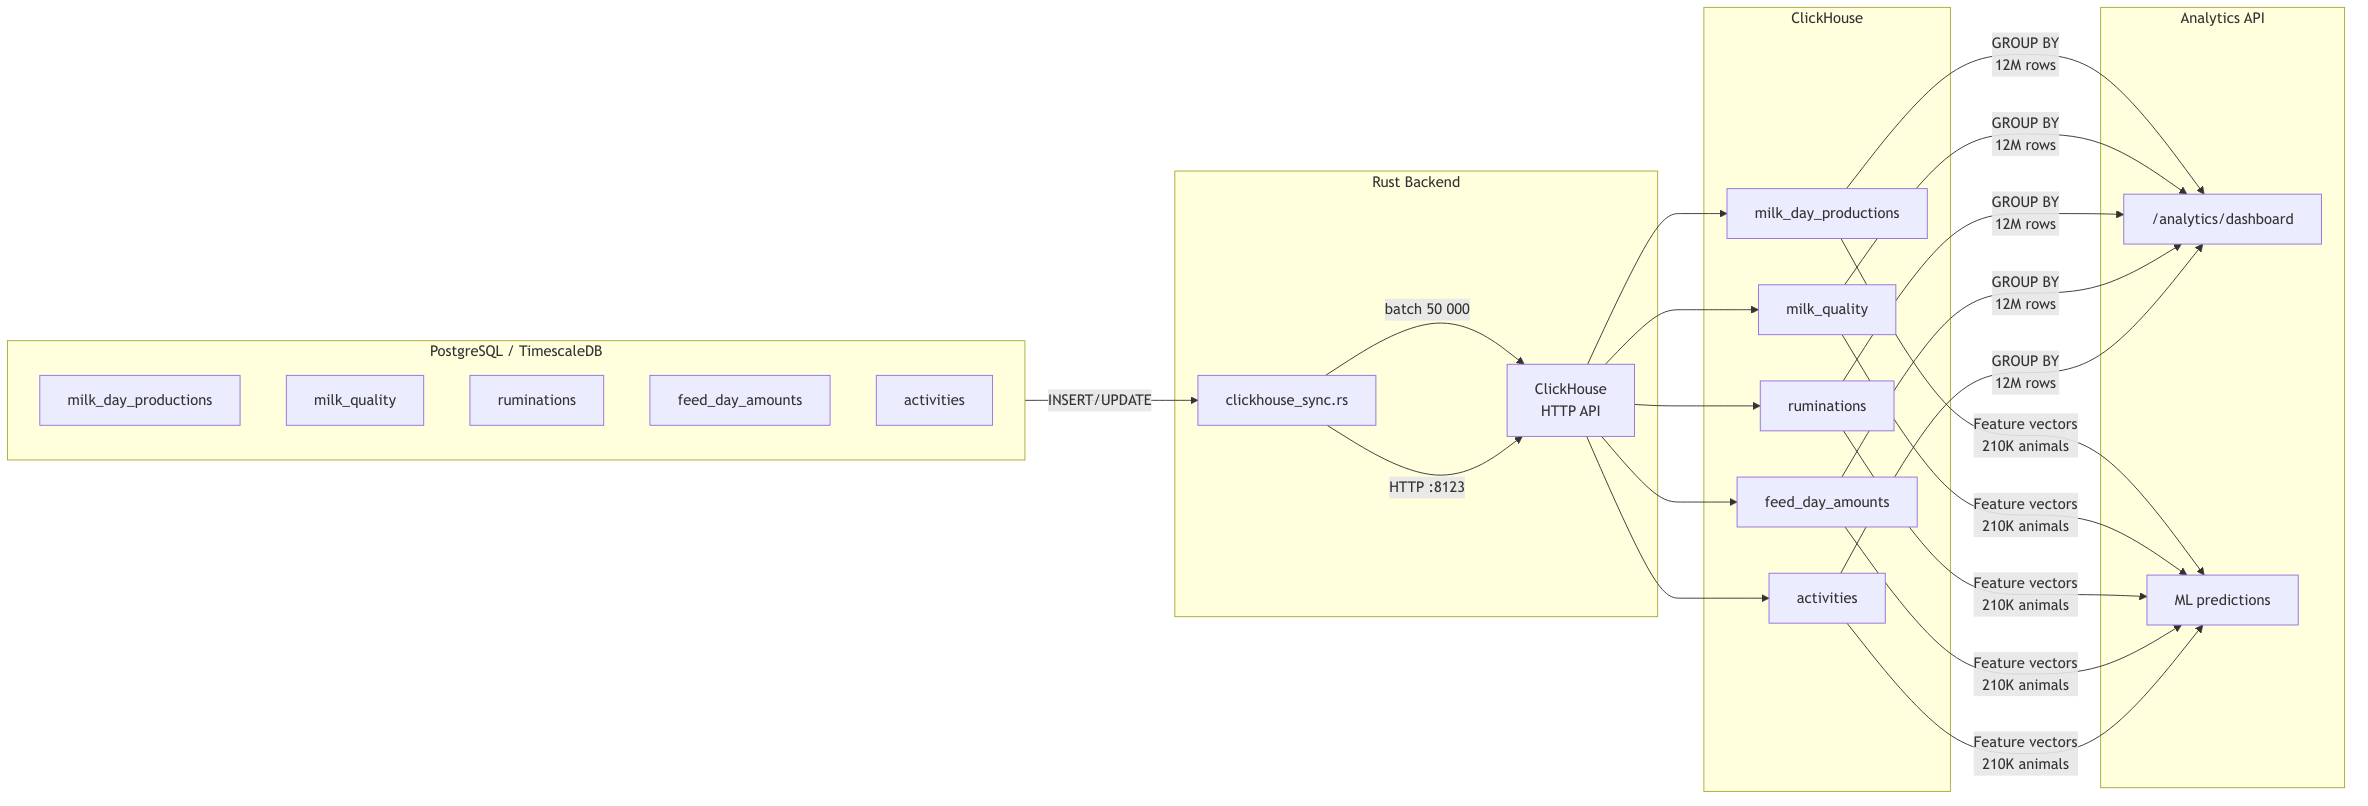
\includegraphics[width=0.85\textwidth,height=0.5\textheight,keepaspectratio]{clickhouse-arch.png}
\caption{Архитектура синхронизации PostgreSQL $\to$ ClickHouse}
\label{fig:clickhouse-arch}
\end{figure}

В таблице~\ref{tab:ch-schema} приведена схема таблиц в ClickHouse.

\begin{table}[htbp]
\caption{Аналитические таблицы ClickHouse}
\label{tab:ch-schema}
\centering
\begin{tabular}{|l|l|c|}
\hline
\textbf{Таблица} & \textbf{Ключ сортировки} & \textbf{Партиция} \\
\hline
\texttt{milk\_day\_productions} & \texttt{(animal\_id, date)} & \texttt{YYYYMM} \\
\hline
\texttt{milk\_quality} & \texttt{(animal\_id, date)} & \texttt{YYYYMM} \\
\hline
\texttt{ruminations} & \texttt{(animal\_id, date)} & \texttt{YYYYMM} \\
\hline
\texttt{feed\_day\_amounts} & \texttt{(animal\_id, date)} & \texttt{YYYYMM} \\
\hline
\texttt{activities} & \texttt{(animal\_id, date)} & \texttt{YYYYMM} \\
\hline
\end{tabular}
\end{table}

Пример запроса к ClickHouse, заменяющего 15 коррелированных подзапросов одним проходом:

\begin{verbatim}
SELECT animal_id,
    avgIf(milk_amount, date >= today() - 7) as avg_milk_7d,
    avgIf(scc, date >= today() - 30)       as avg_scc_30d,
    avgIf(rumination_minutes,
          date >= today() - 7)              as avg_rumination_7d
FROM milk_day_productions m
LEFT JOIN milk_quality q USING (animal_id, date)
LEFT JOIN ruminations r  USING (animal_id, date)
GROUP BY animal_id
\end{verbatim}

\subsubsection{Оптимизация серверной части}

\textbf{Кеширование в Redis.} Реализован модуль \texttt{MlCache} на основе Redis с настраиваемым TTL. Результаты дашборда кешируются на 1~час, результаты ML-предиктов --- на 1~час с ключом, включающим модель и текущий час. При промахе кеша запрос выполняется обычным образом, после чего результат записывается в Redis.

\textbf{Оконные функции вместо коррелированных подзапросов.} Эндпоинт \texttt{health\_timeline} ранее выполнял \texttt{generate\_series} с 4 коррелированными подзапросами на каждый из 365 дней ($365 \times 4 = 1460$ подзапросов). Запрос переписан с использованием оконных функций:

\begin{verbatim}
SELECT date,
  AVG(milk_amount) OVER (
    ORDER BY date ROWS BETWEEN 2 PRECEDING
                        AND CURRENT ROW) as short_milk,
  AVG(milk_amount) OVER (
    ORDER BY date ROWS BETWEEN 29 PRECEDING
                        AND CURRENT ROW) as long_milk,
  STDDEV(milk_amount) OVER (
    ORDER BY date ROWS BETWEEN 29 PRECEDING
                        AND CURRENT ROW) as milk_std
FROM milk_day_productions
WHERE animal_id = $1
ORDER BY date
\end{verbatim}

Такой запрос выполняет один проход по данным вместо 1460 коррелированных подзапросов, что сокращает время выполнения в 10--30 раз.

\textbf{Фоновый мониторинг дрейфа.} Вычисление статистик дрейфа данных (среднее, стандартное отклонение, квантили по 210\,000 строк и 20 признакам) перенесено из синхронного кода в фоновые задачи FastAPI (\texttt{BackgroundTasks}), что устраняет задержку при отправке ответа клиенту.

\subsubsection{Оптимизация клиентского приложения}

Для таблиц с большим количеством строк на странице аналитики применены два подхода:

\begin{enumerate}
    \item \textbf{Реактивные вычисления} --- сортировка и фильтрация данных вынесены в декларативные выражения \texttt{\$derived}, которые вычисляются только при изменении исходных данных, а не при каждом рендеринге компонента.
    \item \textbf{Виртуальный скроллинг} --- библиотека \texttt{svelte-tiny-virtual-list} обеспечивает рендеринг только видимых строк таблицы, что сокращает количество DOM-узлов с тысяч до 20--30 при любой прокрутке.
\end{enumerate}

\subsubsection{Результаты оптимизации}

В таблице~\ref{tab:perf-results} приведено сравнение времени ответа ключевых эндпоинтов до и после оптимизации на наборе данных 10\,435 животных (измерено с помощью \texttt{curl -w}).

\begin{table}[htbp]
\caption{Сравнение времени ответа до и после оптимизации (10\,435 животных)}
\label{tab:perf-results}
\centering
\begin{tabular}{|l|c|c|c|}
\hline
\textbf{Эндпоинт} & \textbf{До, с} & \textbf{После, с} & \textbf{Ускорение} \\
\hline
Дашборд & 5--10 & 0{,}13 & $38--77\times$ \\
\hline
ML-предикт мастита (1 животное) & 5{,}0 & 0{,}04 & $125\times$ \\
\hline
ML-предикт мастита (всё стадо) & 5{,}0 & 4{,}6 & $1{,}1\times$ \\
\hline
ML-предикт эструса (1 животное) & 5{,}0 & 0{,}03 & $167\times$ \\
\hline
ML-предикт кетоза (1 животное) & 1{,}2 & 0{,}02 & $60\times$ \\
\hline
ML-предикт кормления (1 животное) & 0{,}34 & 0{,}01 & $34\times$ \\
\hline
ML-предикт выбраковки (1 животное) & 2{,}3 & 0{,}02 & $115\times$ \\
\hline
Временная шкала здоровья (90 дней) & 10--30 & 0{,}008 & $1250--3750\times$ \\
\hline
\end{tabular}
\end{table}

Основное ускорение при предикте для одного животного достигнуто за счёт фильтрации по \texttt{animal\_id} на уровне SQL-запроса к загрузчику данных (\texttt{WHERE a.id = :aid}), вместо загрузки признаков для всех 10\,435 животных и последующей фильтрации в памяти. Для эндпоинтов, запрашивающих предикт для всего стада, время ответа остаётся значительным (4--5~с), что обусловлено объёмом вычислений для 10\,000+ животных; для таких запросов рекомендуется асинхронный режим с кешированием результата в Redis.

% TODO: uncomment when benchmark data is available
% \begin{figure}[htbp]
% \centering
% \includegraphics[width=0.9\textwidth,height=0.5\textheight,keepaspectratio]{perf-benchmark.png}
% \caption{Результаты нагрузочного тестирования до и после оптимизации}
% \label{fig:perf-benchmark}
% \end{figure}

\subsection{Мониторинг}

Помимо бизнес-логики и аналитики, система включает инфраструктурные компоненты, обеспечивающие её наблюдаемость и надёжную доставку обновлений. Стек мониторинга реализован на базе Grafana LGTM (Loki, Grafana, Tempo, Mimir/Prometheus). На рисунке~\ref{monitoring-arch} представлена архитектура стека мониторинга.

\begin{figure}
  \centering
  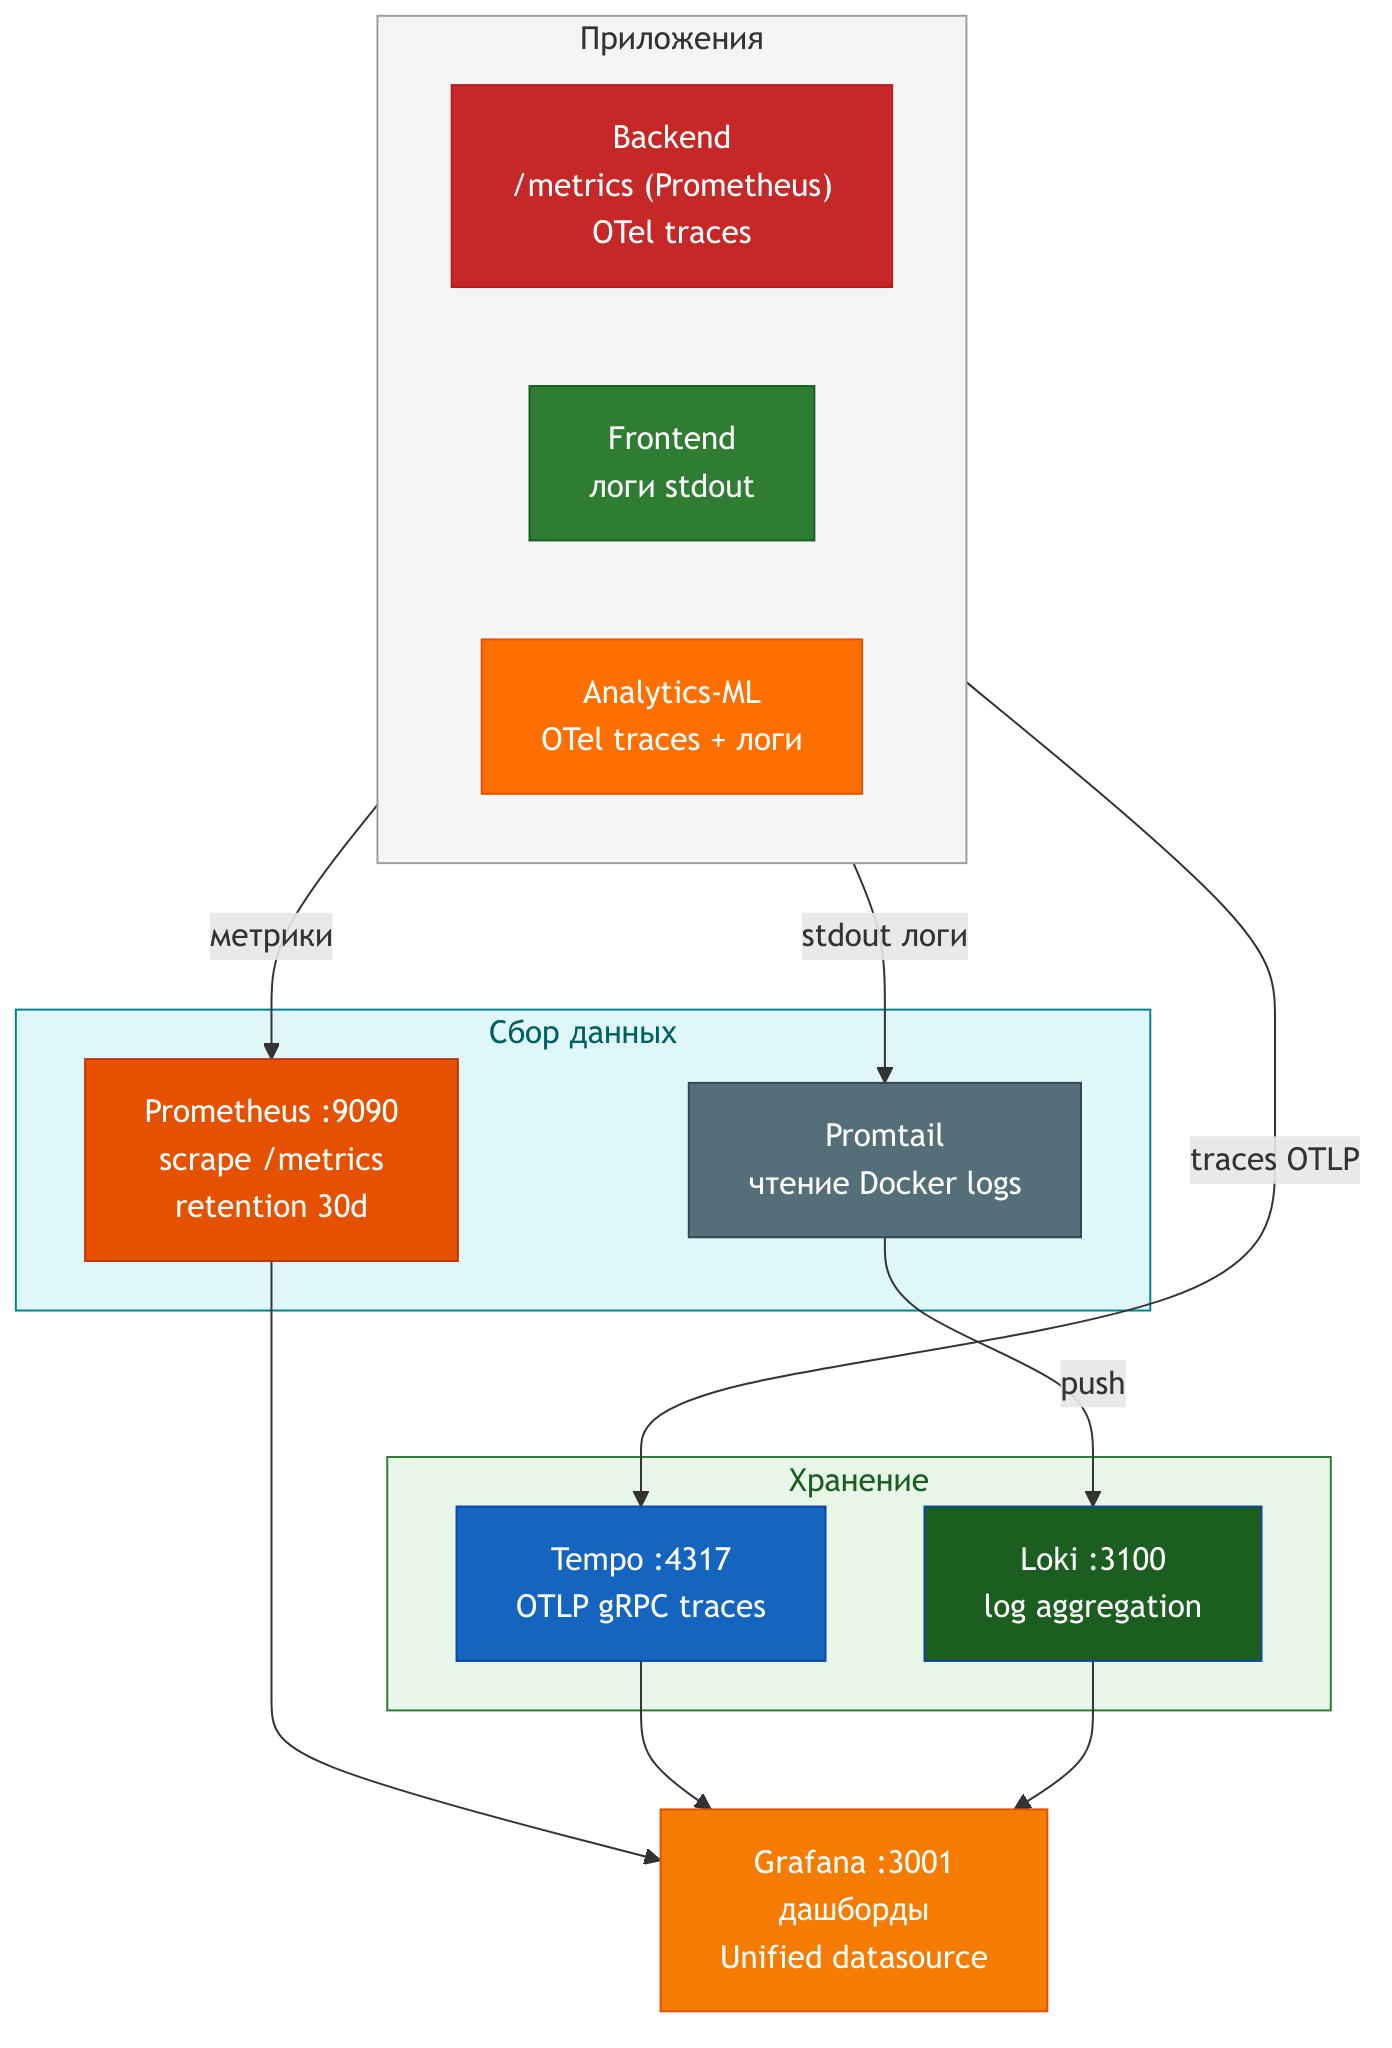
\includegraphics[width=0.95\textwidth,height=0.85\textheight,keepaspectratio]{monitoring.png}
  \caption{Архитектура стека мониторинга}
  \label{monitoring-arch}
\end{figure}

Prometheus~\cite{Prometheus} обеспечивает сбор и хранение метрик с 30-дневным хранением. Grafana~\cite{Grafana} визуализирует дашборды: преднастроенный дашборд backend отображает частоту запросов, время ответа, процент ошибок и использование памяти. Loki~\cite{Loki} агрегирует логи: Promtail собирает логи из Docker-контейнеров, парсит JSON-формат и отправляет в Loki. Tempo~\cite{Tempo} обеспечивает распределённую трассировку через OpenTelemetry OTLP/gRPC, позволяя отследить путь запроса от Nginx через Backend до PostgreSQL.

\subsection{Непрерывная интеграция и доставка (CI/CD)}

Конвейер CI/CD реализован на GitHub Actions~\cite{GHActions}. На рисунке~\ref{cicd} представлена схема конвейера.

\begin{figure}
  \centering
  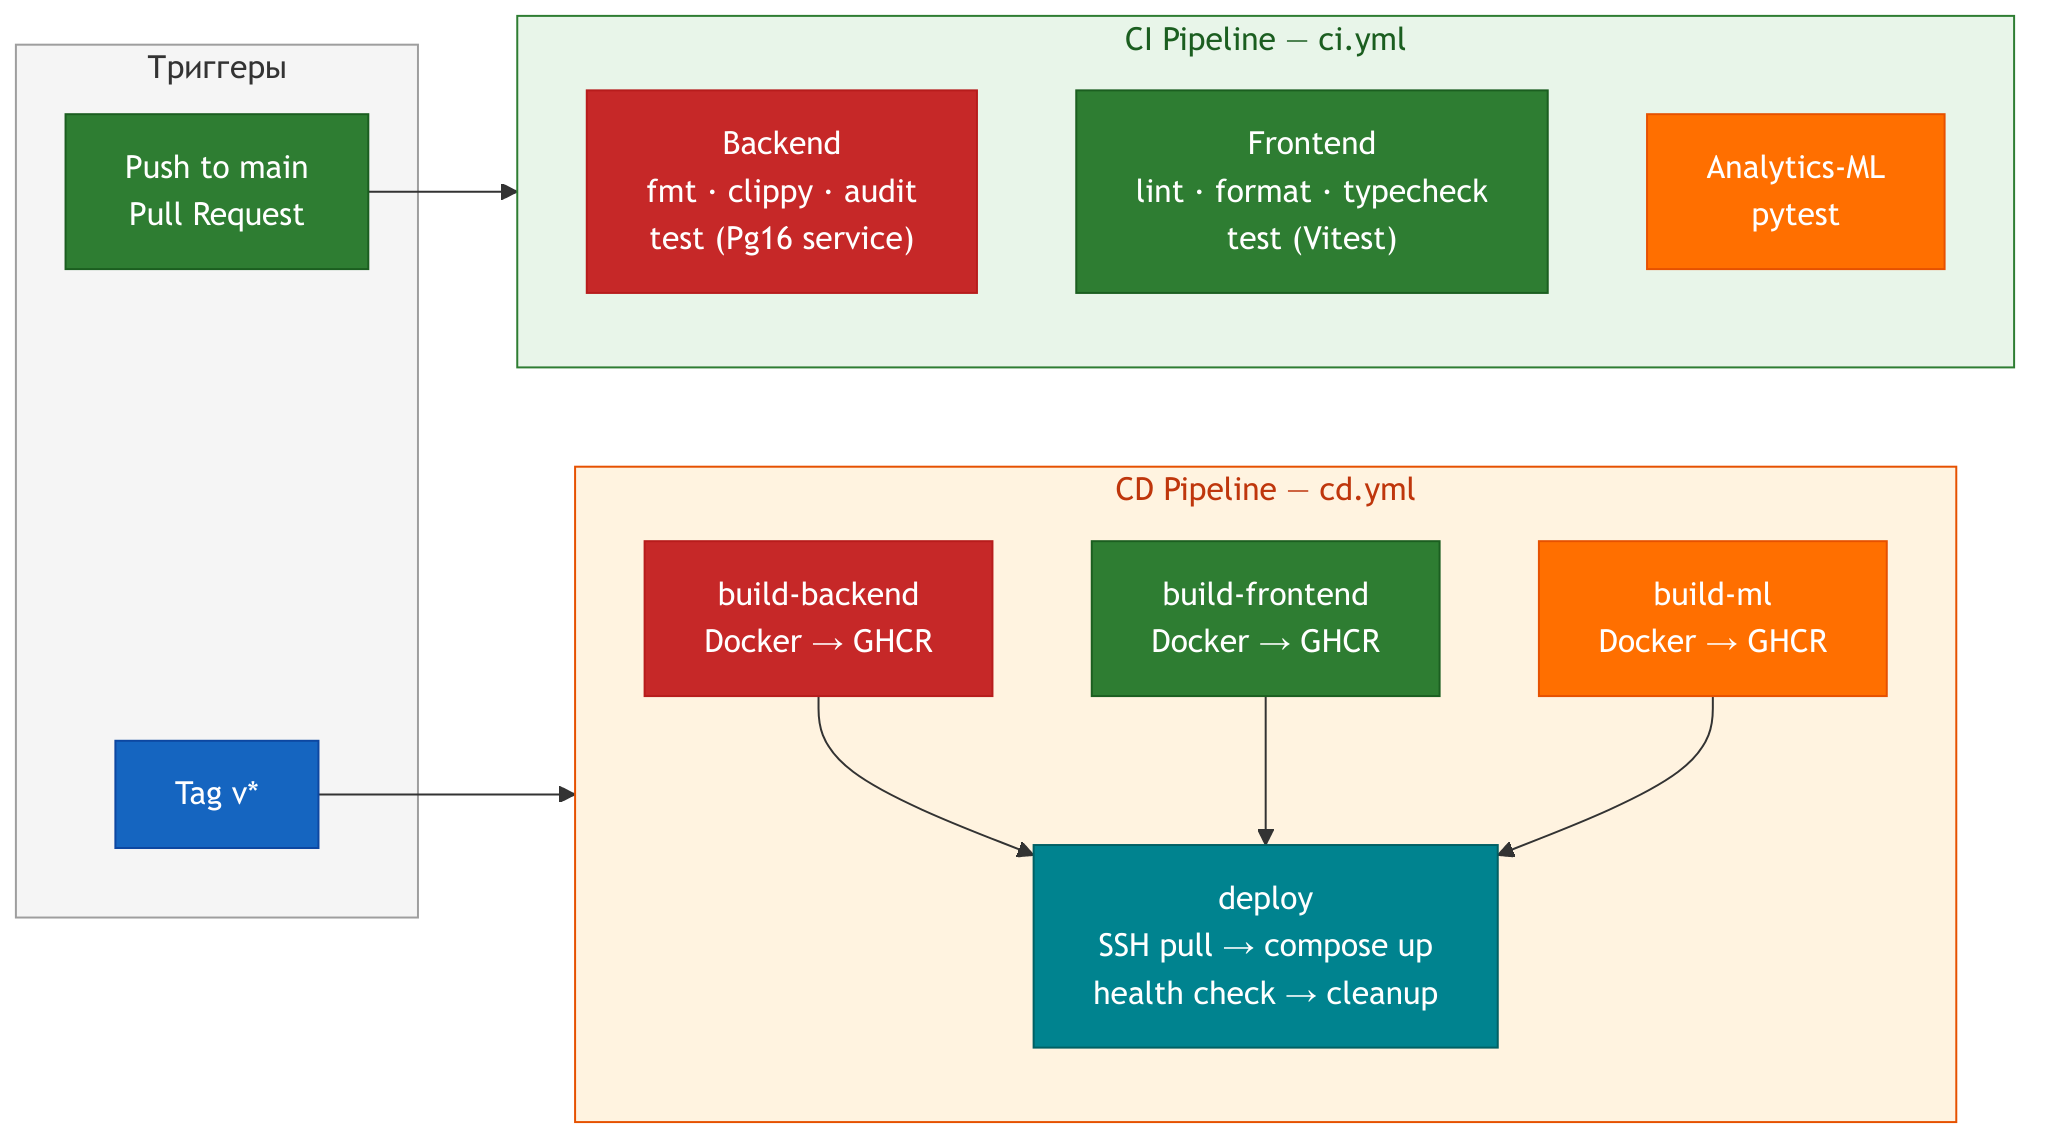
\includegraphics[width=0.95\textwidth,height=0.85\textheight,keepaspectratio]{ci-cd.png}
  \caption{Конвейер непрерывной интеграции и доставки}
  \label{cicd}
\end{figure}

\textbf{Непрерывная интеграция} запускается при каждом push и pull request. Три параллельные задачи: для backend на Rust выполняются проверка форматирования, статический анализ и запуск тестов с PostgreSQL в качестве сервисного контейнера; для frontend на Node.js~20 --- аудит уязвимостей, линтинг, проверка типов и запуск тестов Vitest; для analytics-ml на Python~3.12 --- установка зависимостей и запуск тестов pytest.

\textbf{Непрерывная доставка} запускается при push в main/master или при создании тега \texttt{v*}. Три параллельные задачи сборки Docker-образов публикуются в GHCR~\cite{GHCR}. При создании тега версии дополнительно запускается задача деплоя: SSH на сервер, pull образов, \texttt{docker compose up -d} и проверка работоспособности.

\subsection{Развёртывание}

Для развёртывания используется Docker Compose с двумя конфигурациями. На рисунке~\ref{deploy} представлена схема развёртывания системы.

\begin{figure}
  \centering
  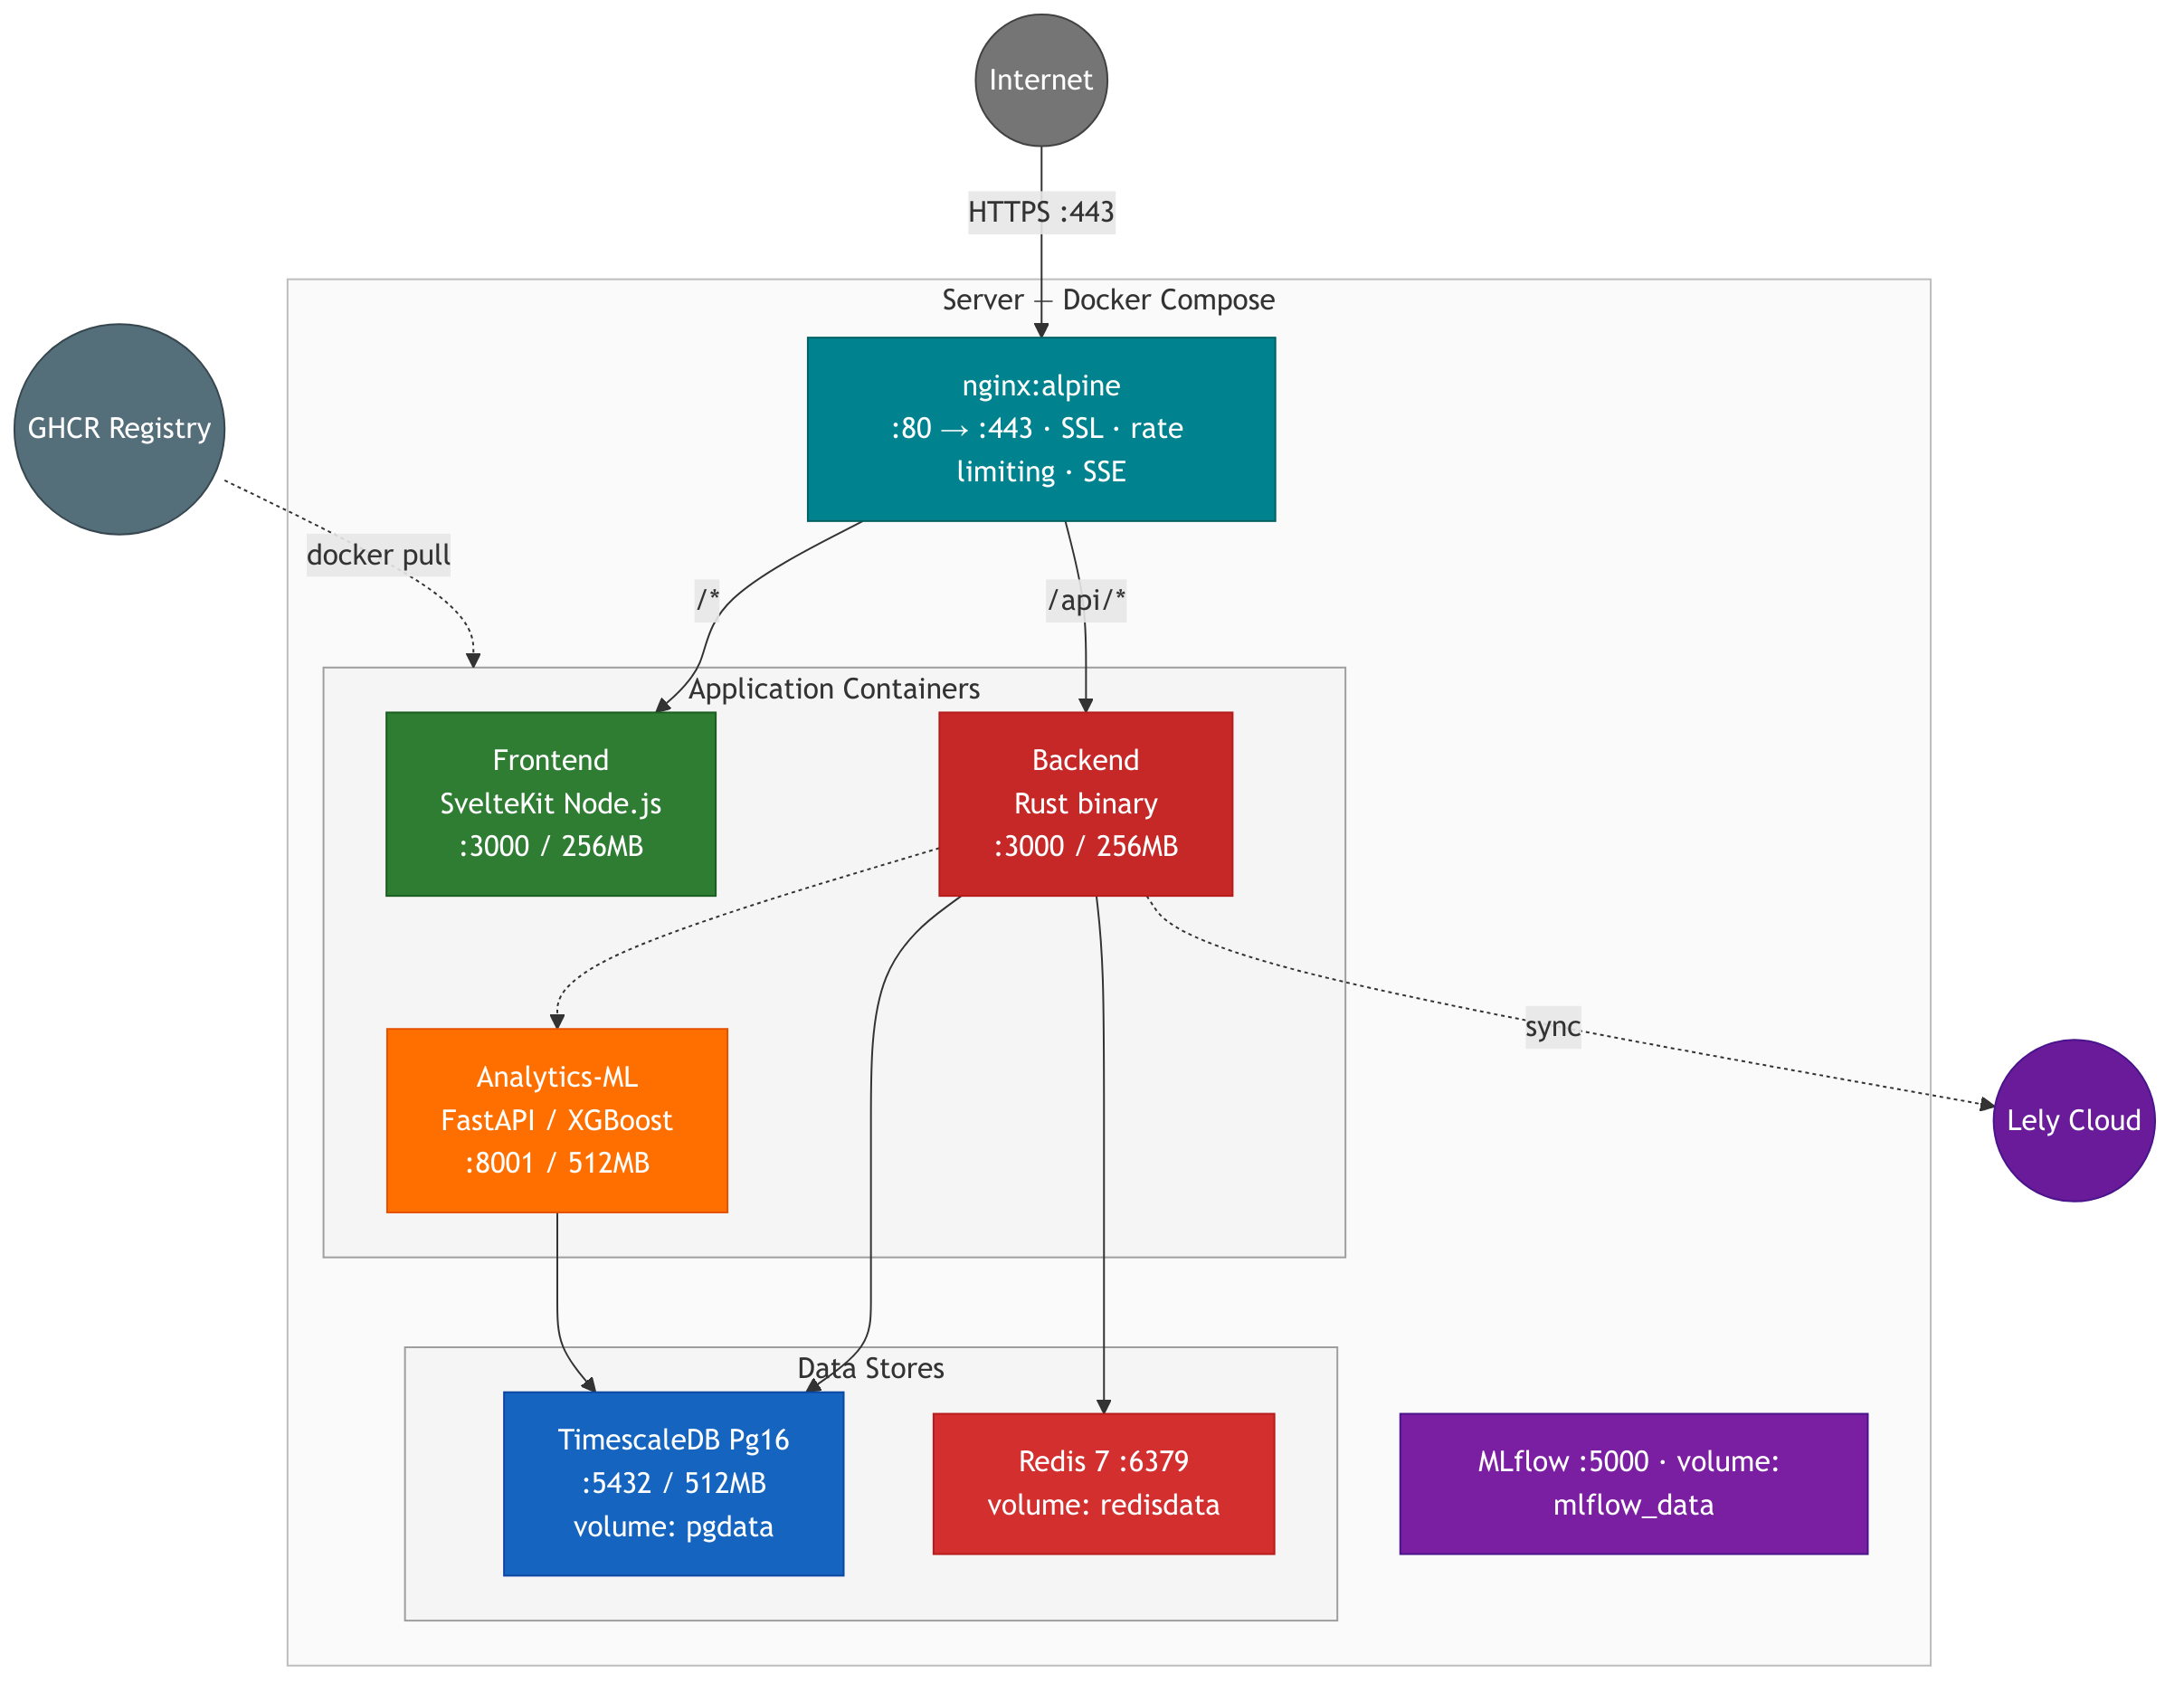
\includegraphics[width=0.95\textwidth,height=0.85\textheight,keepaspectratio]{deployment.png}
  \caption{Схема развёртывания системы}
  \label{deploy}
\end{figure}

\textbf{Разработческая} (\texttt{docker-compose.yml}): 7 сервисов --- PostgreSQL (TimescaleDB), Redis, backend, frontend, Nginx, analytics-ml, MLflow. Nginx на порту 8080.

\textbf{Продуктовая} (\texttt{docker-compose.prod.yml}): те же 7 сервисов с усилением безопасности: переменные окружения через env-файлы, обязательная валидация секретов, \texttt{restart: unless-stopped}, ротация логов, ограничения памяти, SSL-терминация через Nginx с монтированием сертификатов.

Nginx в продуктовой конфигурации обеспечивает: редирект HTTP $\to$ HTTPS, SSL (TLS 1.2/1.3), gzip-сжатие, заголовки безопасности (X-Frame-Options: DENY, HSTS, X-XSS-Protection), rate limiting (30 запросов/сек для API, 5 запросов/сек для auth), кэширование статических ресурсов (30 дней).

\section{ТЕСТИРОВАНИЕ И ДЕМОНСТРАЦИЯ РАБОТЫ СИСТЕМЫ}

\subsection{Стратегия тестирования}

Тестирование разработанной информационной системы включает модульные тесты, интеграционные тесты, сквозные (E2E) тесты и нагрузочное тестирование. Тесты разделены по компонентам системы. Стратегия тестирования основана на пирамиде тестирования: большое количество быстрых модульных тестов, среднее количество интеграционных тестов и небольшое количество E2E-тестов.

В таблице~\ref{testsummary} приведено общее количество тестов по компонентам.

\begin{table}
  \caption{Общее количество тестов по компонентам}
  \begin{tabular}{|l|l|c|}
    \hline
    \textbf{Компонент} & \textbf{Инструмент} & \textbf{Количество файлов} \\
    \hline
    Backend (Rust) & sqlx::test + tower & 17 \\
    \hline
    Frontend (TypeScript) & Vitest + Testing Library & 10 \\
    \hline
    Analytics-ML (Python) & pytest & 3 \\
    \hline
    Нагрузочное тестирование & k6 & 3 \\
    \hline
    E2E & Playwright & 1 \\
    \hline
  \end{tabular}
  \label{testsummary}
\end{table}

\subsection{Тестирование серверной части}

Интеграционные тесты серверной части реализованы с использованием макроса \texttt{sqlx::test}, автоматически подготавливающего тестовую базу данных с применением миграций. HTTP-запросы выполняются in-process через \texttt{tower::ServiceExt}, что исключает сетевые задержки и позволяет тестировать обработчики в изолированной среде.

Тестовый набор включает 17 файлов, покрывающих:
\begin{enumerate}
    \item аутентификацию и авторизацию --- вход с валидными и невалидными учётными данными, выход, обновление токена, проверку ролей admin/user, ограничение частоты попыток входа (5 за 60 секунд), обязательную смену пароля;
    \item CRUD-операции для всех доменных областей --- животные, надои, воспроизводство, кормление, контакты, местоположения, быки, переводы, запасы, включая пакетные операции и импорт CSV;
    \item генерацию отчётов более 17 типов и аналитику --- KPI, тренды, прогнозы;
    \item интеграцию с Lely --- конфигурация, статус синхронизации, ручной запуск;
    \item граничные случаи --- некорректные данные (невалидный JSON, отрицательные значения, строки превышающей длины); конфликты (дублирование инвентарных номеров); несуществующие ресурсы (404); несанкционированный доступ (401, 403).
\end{enumerate}

Для каждого теста создаётся изолированная тестовая база данных, которая уничтожается после выполнения. Общий вспомогательный модуль (\texttt{common/mod.rs}) предоставляет фабрики для создания тестового состояния, генерации JWT-токенов и построения HTTP-запросов.

Пример структуры интеграционного теста: подготовка (создание тестового приложения с подключением к тестовой БД), выполнение (отправка HTTP-запроса к тестируемому эндпоинту), проверка (asserting статус-кода, структуры JSON-ответа и наличия ожидаемых данных) и очистка (тестовая БД уничтожается автоматически).

Помимо функциональных тестов, реализованы бенчмарки для оценки производительности: SQL-запросов (\texttt{bench\_sql}), генерации PDF (\texttt{bench\_pdf}), аутентификации (\texttt{bench\_auth}) и rate limiting (\texttt{bench\_rate\_limit}). Бенчмарки используют критерий Criterion и запускаются командой \texttt{cargo bench}.

\subsection{Тестирование клиентского приложения}

Модульные тесты клиентского приложения реализованы с использованием Vitest~\cite{Vitest} и @testing-library/jest-dom. Тестовый набор включает 10 файлов, покрывающих UI-компоненты (DataTable --- сортировка, пагинация, рендеринг данных; Modal --- открытие, закрытие, контент; FormField --- валидация, отображение ошибок; Pagination --- рендеринг номеров страниц) и утилиты (валидаторы обязательных полей, минимальной длины и формата email; форматирование дат и чисел; построение запросов с параметрами фильтрации и пагинации; хелперы графиков для конфигурации Chart.js; CRUD-модальные окна с состоянием создания и редактирования; бизнес-правила валидации).

Сквозное (E2E) тестирование реализовано с использованием Playwright. Тесты проверяют ключевые пользовательские сценарии: аутентификация (вход с валидными и невалидными данными), навигация по основным разделам, CRUD-операции (создание, редактирование, удаление животного), экспорт отчётов в CSV и PDF.

\subsection{Тестирование модуля машинного обучения}

Тесты модуля машинного обучения включают: test\_api.py --- тесты API-эндпоинтов (проверка health-эндпоинта, вызов прогнозов для всех 11 моделей с валидными и невалидными входными данными, запуск обучения); test\_models.py --- тесты моделей (обучение на синтетических данных, проверка формата прогноза на соответствие JSON-схеме, проверка доверительных интервалов q10 < q50 < q90); test\_drift\_and\_auth.py --- тесты мониторинга дрейфа (обнаружение аномального распределения прогнозов) и аутентификации по API-ключу (отклонение запросов без ключа или с невалидным ключом).

\subsection{Нагрузочное тестирование}

Нагрузочное тестирование проведено с использованием k6~\cite{K6}. Реализованы три сценария: дымовой тест (smoke.js) с 5 виртуальными пользователями и 10 итерациями для проверки health-эндпоинта и входа в систему; нагрузочный тест (load.js), моделирующий типичную рабочую нагрузку с постепенным увеличением числа пользователей от 10 до 50; стресс-тест (stress.js) для определения предельной нагрузки с увеличением числа пользователей до 200.

Метрики, собираемые в ходе нагрузочного тестирования: время ответа (p50, p90, p95), количество запросов в секунду (RPS), процент ошибок (HTTP 5xx), время ожидания соединения (connection time).

\subsection{Демонстрация системы}

Для демонстрации работы системы используется скрипт \texttt{dev.sh}, автоматически запускающий PostgreSQL, разворачивающий тестовые данные и запускающий все компоненты системы. Тестовые данные включают 100 животных с историей надоев, воспроизводства и кормления за 365 дней.

\subsubsection{Аутентификация}

При первом запуске система создаёт пользователя \texttt{admin} со случайным паролем из 16 символов, который выводится в стандартный поток ошибок. При входе в систему, если установлен флаг обязательной смены пароля, пользователь перенаправляется на форму смены пароля. Минимальная длина пароля --- 8 символов. Демонстрация интерфейса аутентификации представлена на рисунке~\ref{auth-page}.

\begin{figure}
  \centering
  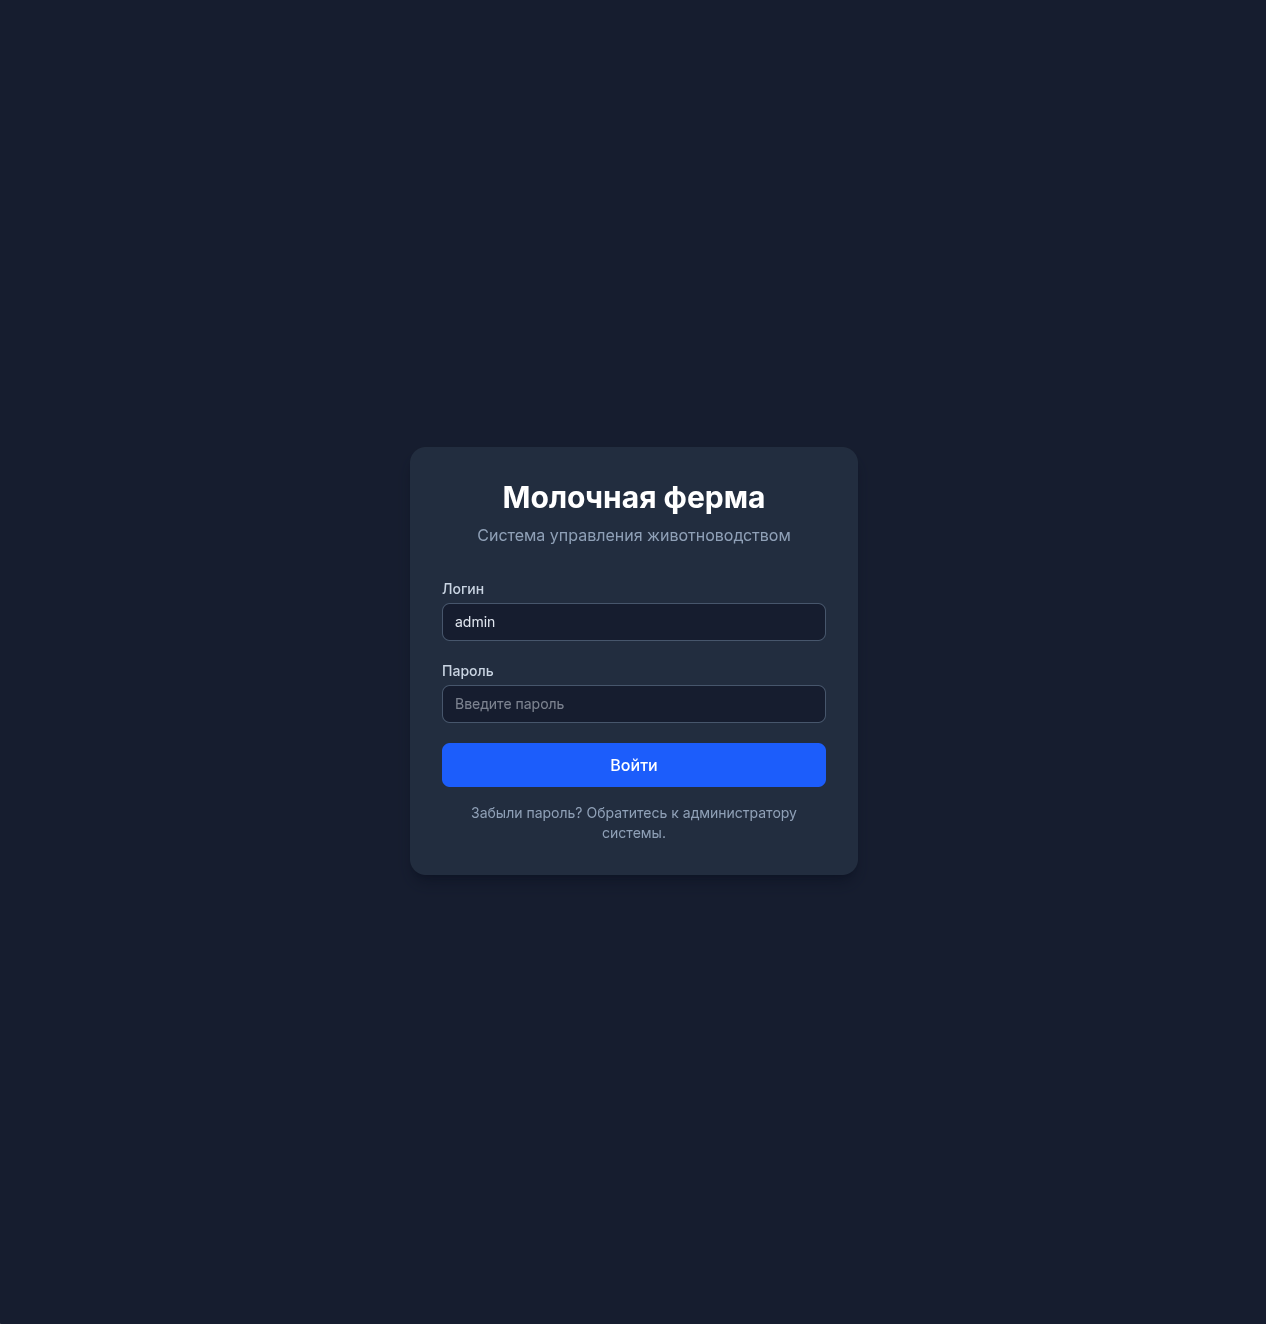
\includegraphics[width=0.95\textwidth,height=0.85\textheight,keepaspectratio]{auth-page-screenshot.png}
  \caption{Страница аутентификации}
  \label{auth-page}
\end{figure}

\subsubsection{Дашборд}

Главная страница системы --- дашборд, отображающий ключевые показатели стада: количество животных (с разбивкой по полу и статусу), средний суточный надой, статус воспроизводства (количество стельных, в охоте, ожидаемых отёлов), количество активных оповещений. Виджеты настраиваются пользователем через панель настроек: можно выбрать отображаемые KPI и их расположение. Пример дашборда представлен на рисунке~\ref{dashboard}.

\begin{figure}
  \centering
  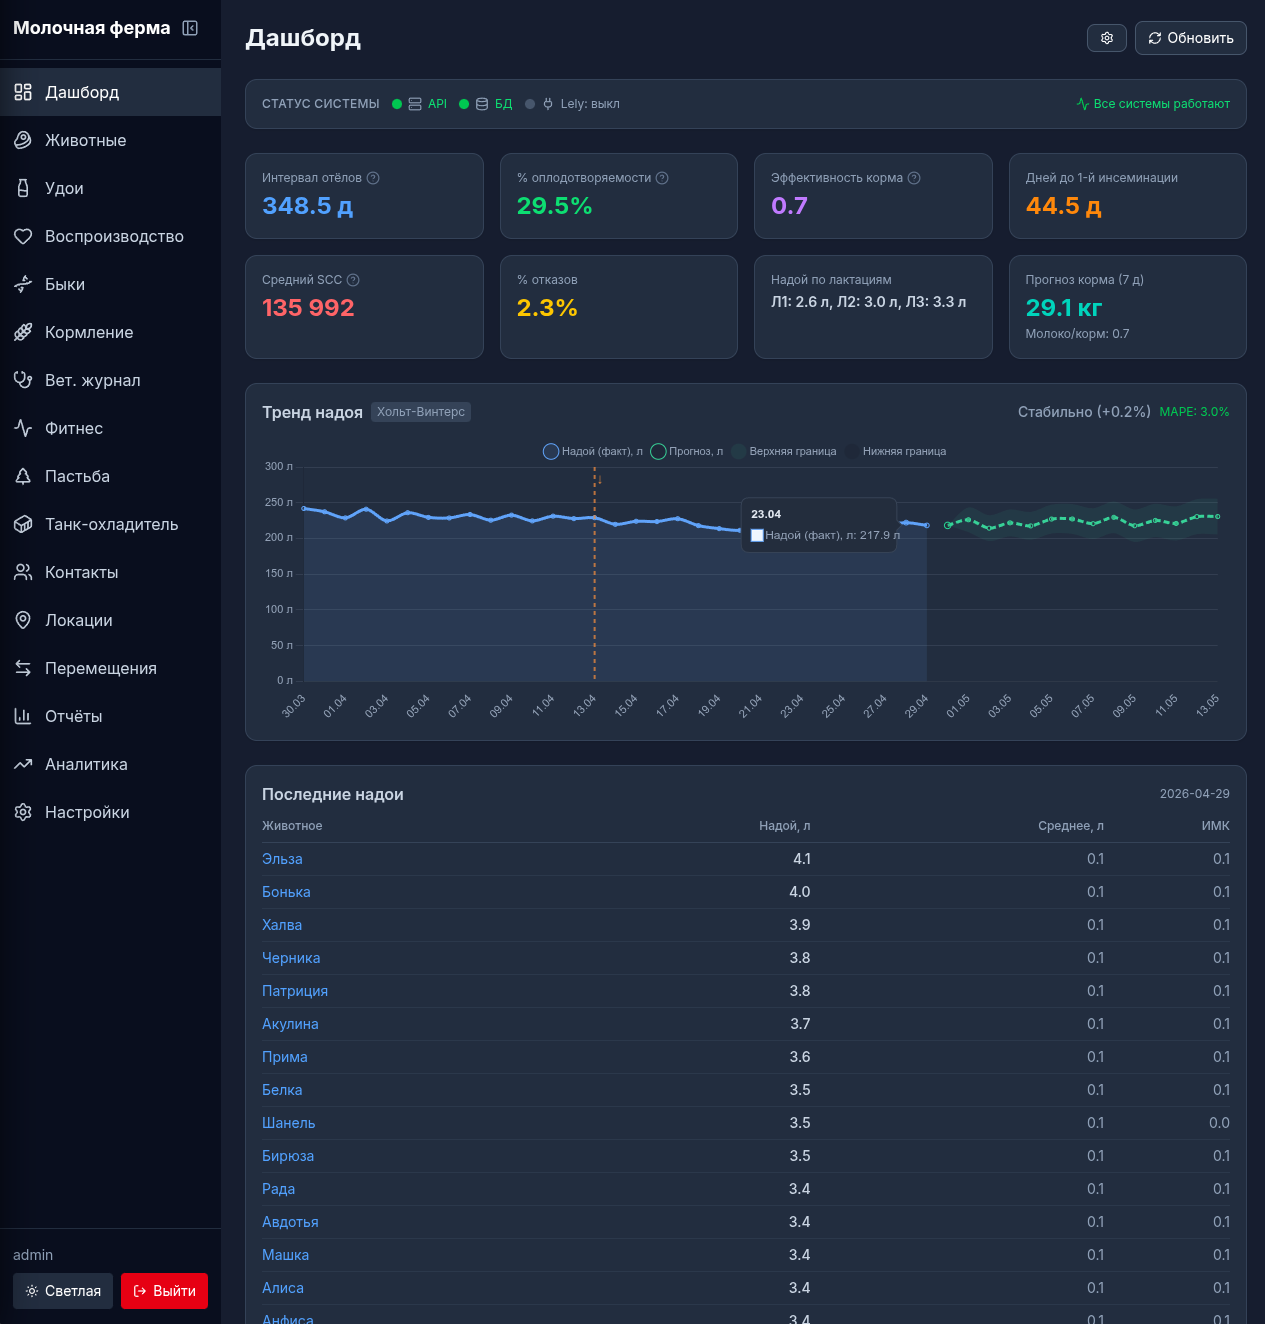
\includegraphics[width=0.95\textwidth,height=0.85\textheight,keepaspectratio]{dashboard-page-screenshot.png}
  \caption{Дашборд системы}
  \label{dashboard}
\end{figure}

\subsubsection{Управление животными}

Страница списка животных предоставляет таблицу с сортировкой по столбцам (кличка, инвентарный номер, пол, дата рождения, статус), фильтрацией (по полу, местоположению, дате рождения) и пагинацией (по 25, 50 или 100 записей). Поддерживается поиск по кличке и инвентарному номеру с использованием нечёткого поиска pg\_trgm (триграммное сходство).

Для каждого животного доступна детальная карточка с полной информацией, разделённой на вкладки: биография (основные данные, происхождение), надои (графики и таблица), воспроизводство (история событий), кормление (план и факт), ветеринарные записи. Поддерживается экспорт карточки в PDF. Пример списка животных представлен на рисунке~\ref{animals-page}, пример детальной карточки --- на рисунке~\ref{animal-card}.

\begin{figure}
  \centering
  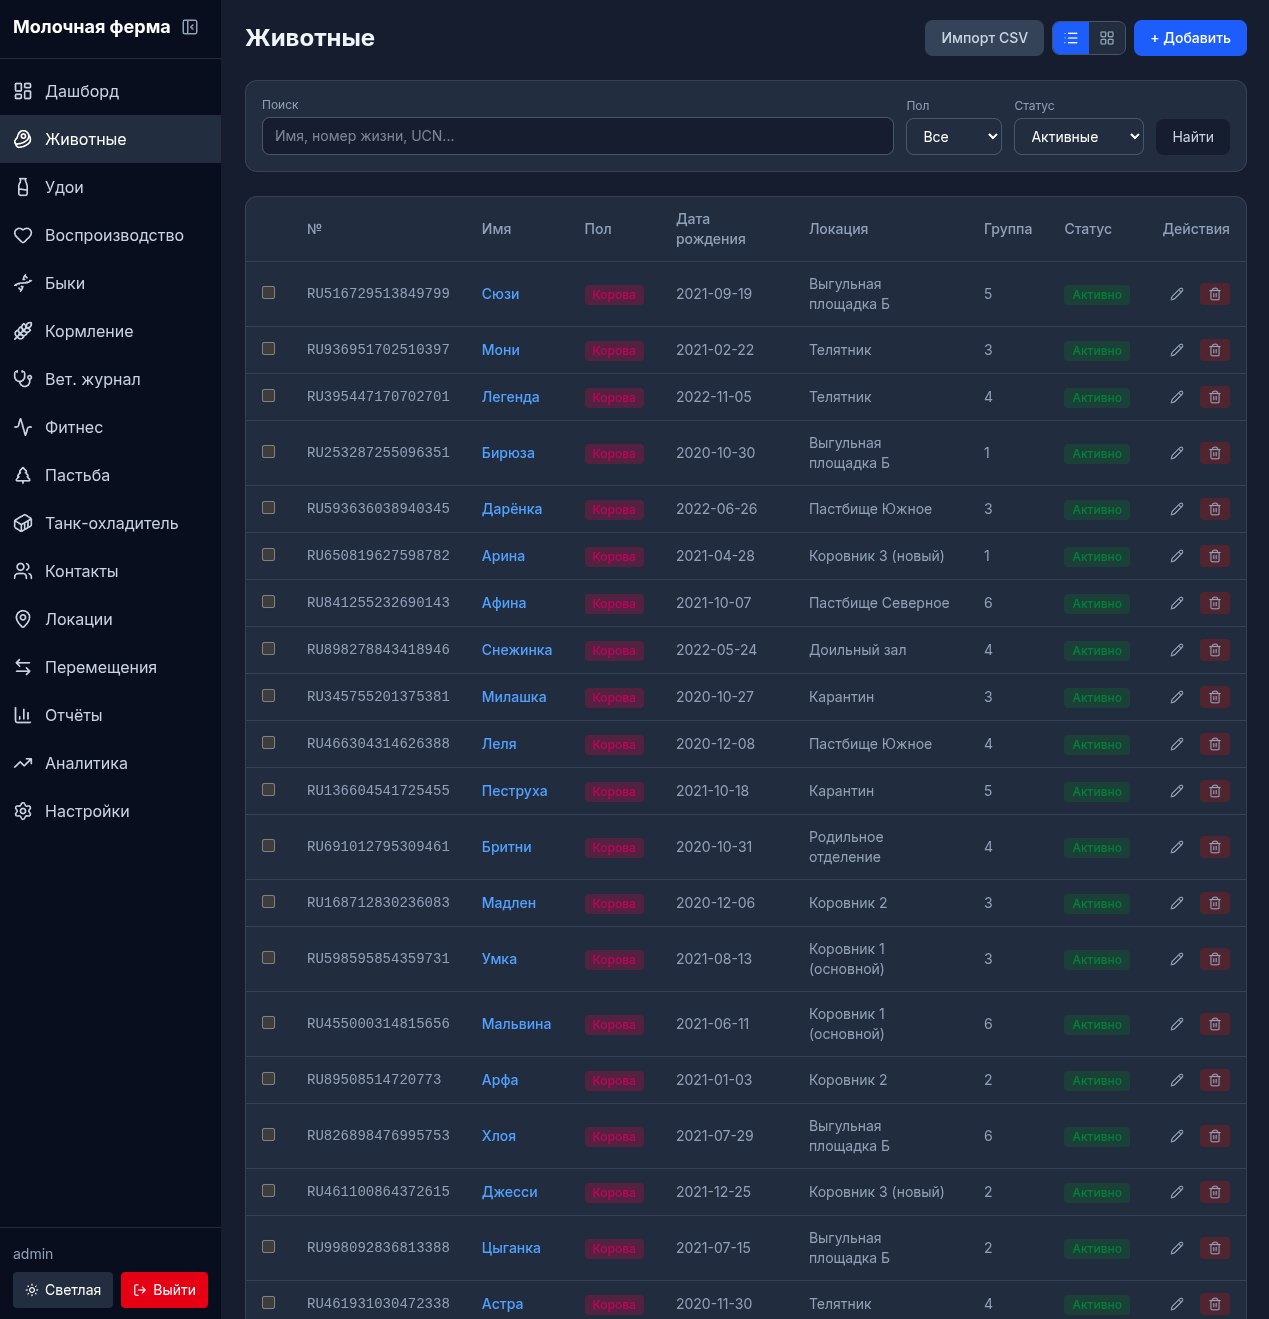
\includegraphics[width=0.95\textwidth,height=0.85\textheight,keepaspectratio]{animals-page-screenshot.png}
  \caption{Список животных}
  \label{animals-page}
\end{figure}

\begin{figure}
  \centering
  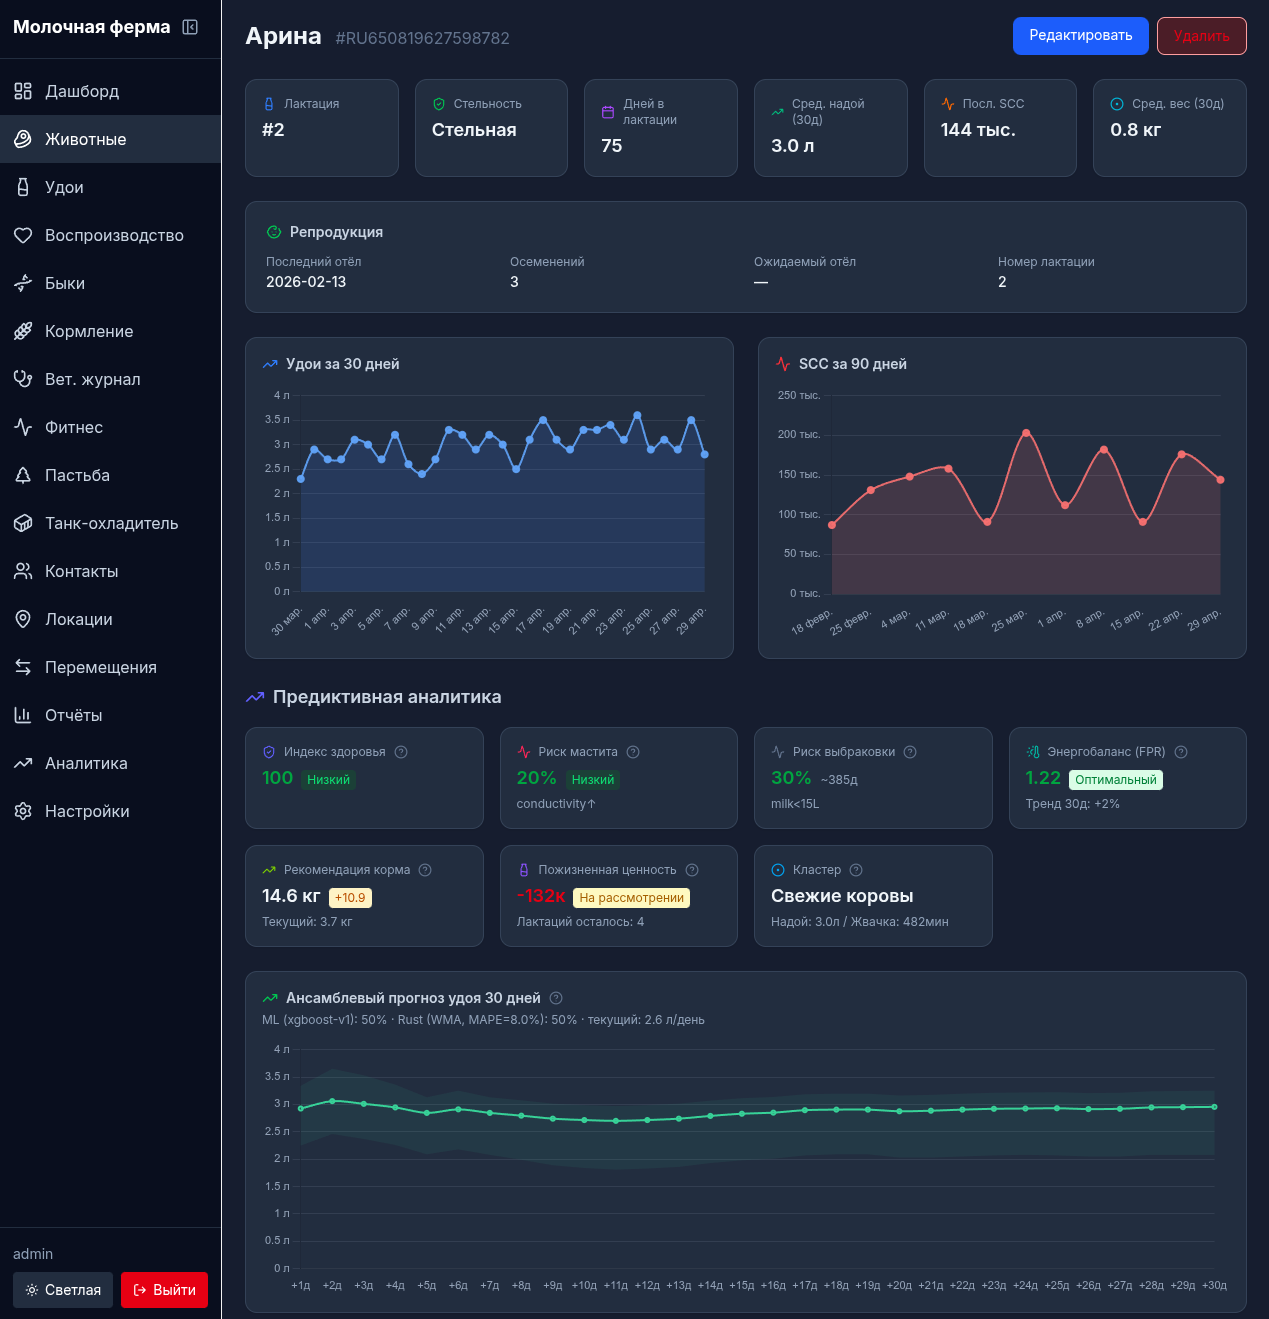
\includegraphics[width=0.95\textwidth,height=0.85\textheight,keepaspectratio]{animal-card-screenshot.png}
  \caption{Детальная карточка животного}
  \label{animal-card}
\end{figure}

\subsubsection{Отчёты и аналитика}

Система генерирует более 17 типов отчётов (см. таблицу~\ref{reports}), каждый из которых отображается в виде таблицы и/или графика в интерфейсе. Отчёты поддерживают фильтрацию по дате и группе животных, а также экспорт в CSV и PDF.

Аналитическая панель отображает: ключевые показатели эффективности (KPI) --- средний надой, процент стельных, интервал между отёлами; тренды надоев с прогнозом на основе модели Хольта--Винтерса; прогноз стельных коров; кривые лактации по номерам; кластеризацию стада.

\subsubsection{Интеграция с Lely}

При включённой интеграции с Lely система автоматически синхронизирует данные каждые 5 минут. Страница статуса синхронизации отображает дату последней успешной синхронизации для каждого из 23 типов данных и количество синхронизированных записей. Через интерфейс доступен ручной запуск синхронизации и просмотр логов синхронизации.

\subsubsection{Оповещения}

Модуль оповещений автоматически создаёт оповещения на основе настраиваемых пороговых значений. Проверка выполняется каждые 15 минут фоновым заданием. Отслеживаются следующие категории событий:
\begin{enumerate}
    \item падение надоев более чем на 20~процентов за сутки;
    \item высокий \acrshort{scc} (более 200\,000 клеток/мл);
    \item снижение активности более чем на 30~процентов за сутки;
    \item снижение жвачки более чем на 25~процентов за сутки;
    \item ожидаемый отёл (за 7 дней до планируемой даты).
\end{enumerate}

Пороговые значения настраиваются через страницу настроек без перезапуска сервера. Оповещения отображаются в интерфейсе с категоризацией по степени важности (high, medium, low). Поддерживается подтверждение оповещения (acknowledge) для отслеживания реакции фермера. Оповещения также могут быть отправлены через канал уведомлений (браузерные уведомления или Telegram-бот).

\subsection{Мониторинг работоспособности}

Стек Grafana LGTM обеспечивает комплексное наблюдение за системой. Grafana дашборды отображают частоту запросов, время ответа (p50, p95, p99), использование ресурсов (CPU, память) и ошибки по маршрутам. Loki позволяет искать логи по уровню (info, warn, error) и целевому сервису с использованием языка LogQL. Tempo обеспечивает распределённую трассировку запросов через цепочку Nginx $\to$ Backend $\to$ PostgreSQL/ML, позволяя идентифицировать медленные запросы. Prometheus собирает метрики с backend (\texttt{/metrics}), analytics-ml (\texttt{/metrics}) и Redis с интервалом 15 секунд.

Метрики backend включают: \texttt{http\_requests\_total} (счётчик, разбитый по маршруту, методу и статус-коду), \texttt{http\_request\_duration\_seconds} (гистограмма), \texttt{db\_connections\_active}, \texttt{rate\_limit\_rejections\_total}.


\conclusion

В результате выполнения выпускной квалификационной работы бакалавра была разработана информационная система управления молочной фермой с интеграцией роботизированного доильного оборудования Lely и предиктивной аналитикой на основе моделей машинного обучения. Все поставленные задачи были выполнены.

Проведён анализ предметной области и существующих решений (Lely Horizon, DeLaval DelPro, SCR Heatime, 1С: Управление фермой), показавший, что ни одно из них не обеспечивает одновременно полный цикл управления стадом, интеграцию с оборудованием сторонних производителей, встроенные модели машинного обучения и открытую архитектуру. На основании анализа сформулировано техническое задание и обоснован выбор стека технологий (Rust/Axum, SvelteKit, Python/FastAPI, PostgreSQL/TimescaleDB).

Спроектирована и реализована трёхзвенная архитектура. Серверная часть на Rust/Axum включает 25 модулей обработчиков, 33 модуля сервисов, 24 модуля моделей данных и 6 модулей middleware. Аутентификация на основе JWT с HttpOnly cookie обеспечивает защиту от CSRF и XSS. Middleware-стек включает rate limiting (Redis/in-memory), gzip-сжатие, CSRF-защиту, метрики Prometheus и распределённую трассировку. База данных PostgreSQL содержит более 35 таблиц с расширением TimescaleDB для эффективной работы с временными рядами.

Реализована интеграция с облачным API Lely Horizon, обеспечивающая автоматическую двустороннюю синхронизацию 23 типов данных (животные, надои, воспроизводство, кормление, фитнес, оборудование) с шифрованием учётных данных AES-256-GCM и инкрементальной синхронизацией по временным диапазонам.

Клиентское веб-приложение на SvelteKit~5 содержит более 24 страниц с серверным рендерингом и адаптивным интерфейсом на Tailwind CSS. Разработано более 16 переиспользуемых UI-компонентов, включая DataTable с серверной пагинацией и адаптивным отображением, компоненты визуализации на Chart.js (надои, SCC, лактационные кривые, прогнозы), систему уведомлений и валидацию форм на основе реактивных Runes.

Модуль машинного обучения на Python/FastAPI включает 11 моделей: прогноз надоев на корову (XGBoost с квантильной регрессией q10/q50/q90, обеспечивающей доверительные интервалы) и на стадо (Prophet с декомпозицией тренда и сезонности), обнаружение мастита и кетоза, выявление охоты, оценка риска выбраковки, оценка BCS, кластеризация стада (KMeans с автоматическим выбором $k$ по силуэту), аномалии оборудования (Isolation Forest) и рекомендации по кормлению. MLOps-инфраструктура включает: автоматическое переобучение (APScheduler), оптимизацию гиперпараметров (Optuna, TPE-сэмплер, 8-мерное пространство), мониторинг дрейфа данных (prediction drift и feature drift), версионирование моделей и отслеживание экспериментов (MLflow).

В серверной части реализованы алгоритмы предиктивной аналитики на Rust: метод Хольта--Винтерса для прогнозирования временных рядов надоя с обнаружением выбросов (IQR) и структурных сдвигов (t-критерий); кривая лактации Вуда для моделирования зависимости надоя от DIM; комплексный индекс здоровья на основе Z-оценок четырёх показателей (надой, жвачка, активность, SCC) с динамической визуализацией тренда за 90 дней; оптимизатор запуска; система сравнения 8 моделей прогнозирования (SES, SMA, WMA, линейная регрессия, метод Хольта, Хольт--Винтерс, ряд Фурье, ARIMA(0,1,1)) с автоматическим выбором лучшей по MAPE. Реализован ансамблевый прогноз, объединяющий ML-модель (XGBoost) и лучшую Rust-модель методом взвешенного среднего с весами, обратно пропорциональными MAPE, что повышает робастность прогнозирования. Для обеспечения интерпретируемости прогнозов внедрён метод SHAP, визуализирующий вклад каждого признака в виде горизонтальной столбчатой диаграммы в интерфейсе.

Основные количественные результаты разработки включают: серверную часть из 25 модулей обработчиков, 33 модулей сервисов, 24 модулей моделей данных и 6 модулей middleware; базу данных из более 35 таблиц, более 20 файлов миграций с расширениями TimescaleDB и pg\_trgm; клиентское приложение из более 24 страниц, 23 модулей API-клиента и более 16 UI-компонентов; модуль машинного обучения из 11 моделей с автоматическим обучением и переобучением, мониторингом дрейфа и оптимизацией гиперпараметров через Optuna; серверную аналитику из 8 моделей прогнозирования с автоматическим сравнением по MAPE/RMSE, индексом здоровья и кривой Вуда; интеграцию с Lely, охватывающую 23 типа синхронизируемых данных с шифрованием AES-256-GCM и инкрементальной синхронизацией; мониторинг через стек Grafana LGTM для сбора метрик, логов и трассировок; тестирование из 30+ тестовых файлов с нагрузочным тестированием через k6; и конвейер CI/CD с параллельным тестированием трёх компонентов и автоматическим деплоем при создании тегов.

Научная новизна работы заключается в архитектурном решении, позволяющем серверным алгоритмам прогнозирования на Rust работать автономно, обеспечивая предиктивную аналитику даже при недоступности ML-сервиса, а также в реализации системы автоматического сравнения 8 моделей прогнозирования с выбором оптимальной для каждого животного индивидуально и ансамблевого объединения прогнозов ML и Rust-моделей с весами, обратно пропорциональными MAPE.

Практическая значимость подтверждается полнотой покрытия бизнес-процессов молочной фермы: от учёта животных и надоев до предиктивной аналитики и интеграции с роботизированным оборудованием. Система развёрнута в контейнерах Docker с обратным прокси Nginx, SSL-терминацией и мониторингом, что обеспечивает готовность к промышленной эксплуатации.

Дальнейшее развитие системы может включать: расширение набора моделей машинного обучения (прогнозирование заболеваемости конечностей, оптимизация параметров доильных роботов); интеграцию с дополнительными производителями оборудования (DeLaval, GEA); разработку мобильного приложения для фермеров с push-уведомлениями; добавление модулей финансового анализа и планирования с учётом стоимости кормов, ветеринарных услуг и рыночных цен на молоко; внедрение online learning для адаптации моделей к новым данным в реальном времени.


\printbibliography

\appendix
\appendixsection{Исходный код}

На рисунке~\ref{qr} изображён QR-код со ссылкой на GitHub репозиторий с исходным кодом разработанной информационной системы.

\begin{figure}
    
\includegraphics[height=0.4\textheight]{QR-for-antonprdx.png}
    \caption{QR-код на репозиторий}
    \label{qr}
\end{figure}

\appendixsection{Описание таблиц базы данных}
\label{app-db}

В данном приложении приведён перечень основных таблиц базы данных PostgreSQL с указанием назначения и ключевых полей.

В таблице~\ref{dbtables1} представлены таблицы учёта и воспроизводства.

\begin{table}
  \caption{Таблицы учёта животных и воспроизводства}
  \begin{tabular}{|l|p{8cm}|}
    \hline
    \textbf{Таблица} & \textbf{Назначение} \\
    \hline
    users & Пользователи: username, password\_hash, role \\
    \hline
    animals & Реестр животных: life\_number, name, gender, birth\_date, active \\
    \hline
    sires & Быки-производители: name, code, breed \\
    \hline
    calvings & Отёлы: animal\_id, date, calf\_id \\
    \hline
    calves & Телята: calving\_id, life\_number, gender \\
    \hline
    inseminations & Осеменения: animal\_id, date, sire\_id \\
    \hline
    pregnancies & Стельности: animal\_id, date, expected\_due\_date \\
    \hline
    heats & Охоты: animal\_id, date, activity\_level \\
    \hline
    dry\_offs & Запуски: animal\_id, date \\
    \hline
    transfers & Переводы: animal\_id, from\_location, to\_location \\
    \hline
    bloodlines & Кровные линии: animal\_id, sire\_id, dam\_id \\
    \hline
    locations & Местоположения: name, type, capacity \\
    \hline
    contacts & Контакты: name, phone, role \\
    \hline
  \end{tabular}
  \label{dbtables1}
\end{table}

В таблице~\ref{dbtables2} представлены таблицы надоев, кормления и мониторинга.

\begin{table}
  \caption{Таблицы надоев, кормления и мониторинга}
  \begin{tabular}{|l|p{8cm}|}
    \hline
    \textbf{Таблица} & \textbf{Назначение} \\
    \hline
    milk\_day\_productions & Суточные надои: animal\_id, date, milk\_kg, fat, protein, scc \\
    \hline
    milk\_visits & Визиты на доение: animal\_id, start\_time, milk\_kg, robot\_id \\
    \hline
    milk\_quality & Качество молока: animal\_id, date, scc, fat, protein \\
    \hline
    milk\_visit\_quality & Качество по визитам: visit\_id, scc, conductivity \\
    \hline
    robot\_milk\_data & Данные роботов: visit\_id, quarter\_times \\
    \hline
    feed\_types & Типы кормов: name, cost, unit \\
    \hline
    feed\_groups & Группы кормов: type\_id, group\_name \\
    \hline
    feed\_day\_amounts & Дневные объёмы: animal\_id, planned\_kg, actual\_kg \\
    \hline
    feed\_visits & Визиты на кормление: animal\_id, time, amount\_kg \\
    \hline
    activities & Активность: animal\_id, date, steps \\
    \hline
    ruminations & Жвачка: animal\_id, date, minutes \\
    \hline
    grazing\_data & Пастьба: animal\_id, date, hours \\
    \hline
    bulk\_tank\_tests & Резервуар: date, volume, temperature \\
    \hline
  \end{tabular}
  \label{dbtables2}
\end{table}

В таблице~\ref{dbtables3} представлены системные таблицы.

\begin{table}
  \caption{Системные таблицы}
  \begin{tabular}{|l|p{8cm}|}
    \hline
    \textbf{Таблица} & \textbf{Назначение} \\
    \hline
    alerts & Оповещения: animal\_id, category, severity, status \\
    \hline
    tasks & Задачи: title, assignee, status, priority \\
    \hline
    audit\_log & Аудит: user\_id, action, entity, timestamp \\
    \hline
    inventory\_items & Запасы: name, quantity, unit \\
    \hline
    inventory\_transactions & Операции с запасами: item\_id, type, quantity \\
    \hline
    vet\_records & Ветеринария: animal\_id, date, diagnosis \\
    \hline
    lely\_config & Конфигурация Lely: base\_url, encrypted\_credentials \\
    \hline
    lely\_sync\_state & Состояние синхронизации: entity\_type, last\_sync\_at \\
    \hline
    system\_settings & Настройки: key, value \\
    \hline
    user\_preferences & Предпочтения: user\_id, theme, page\_size \\
    \hline
    revoked\_tokens & Отозванные токены: jti, expires\_at \\
    \hline
    weather\_cache & Кэш погоды: date, temperature \\
    \hline
    farm\_zones & Зоны фермы: name, type, boundaries \\
    \hline
    culling\_events & Выбраковки: animal\_id, date, reason \\
    \hline
  \end{tabular}
  \label{dbtables3}
\end{table}

\appendixsection{Визуализация модели данных}
\label{app-er}

В данном приложении представлена полная модель данных информационной системы в виде ER-диаграмм, разделённых по предметным областям. Диаграммы отображают все 35+ таблиц базы данных PostgreSQL, их ключевые столбцы и отношения между таблицами. Таблицы, отмеченные символом $\rightleftharpoons$, являются гипертаблицами TimescaleDB с автоматической партицировкой по времени.

\textbf{Пользователи и реестр животных}

На рисунке~\ref{er-core} представлены основные таблицы пользователей и реестра животных. Таблица \texttt{animals} является центральной сущностью системы, на которую ссылается большинство остальных таблиц через внешний ключ \texttt{animal\_id}. Таблица \texttt{users} обеспечивает аутентификацию и авторизацию.

\begin{figure}
  \centering
  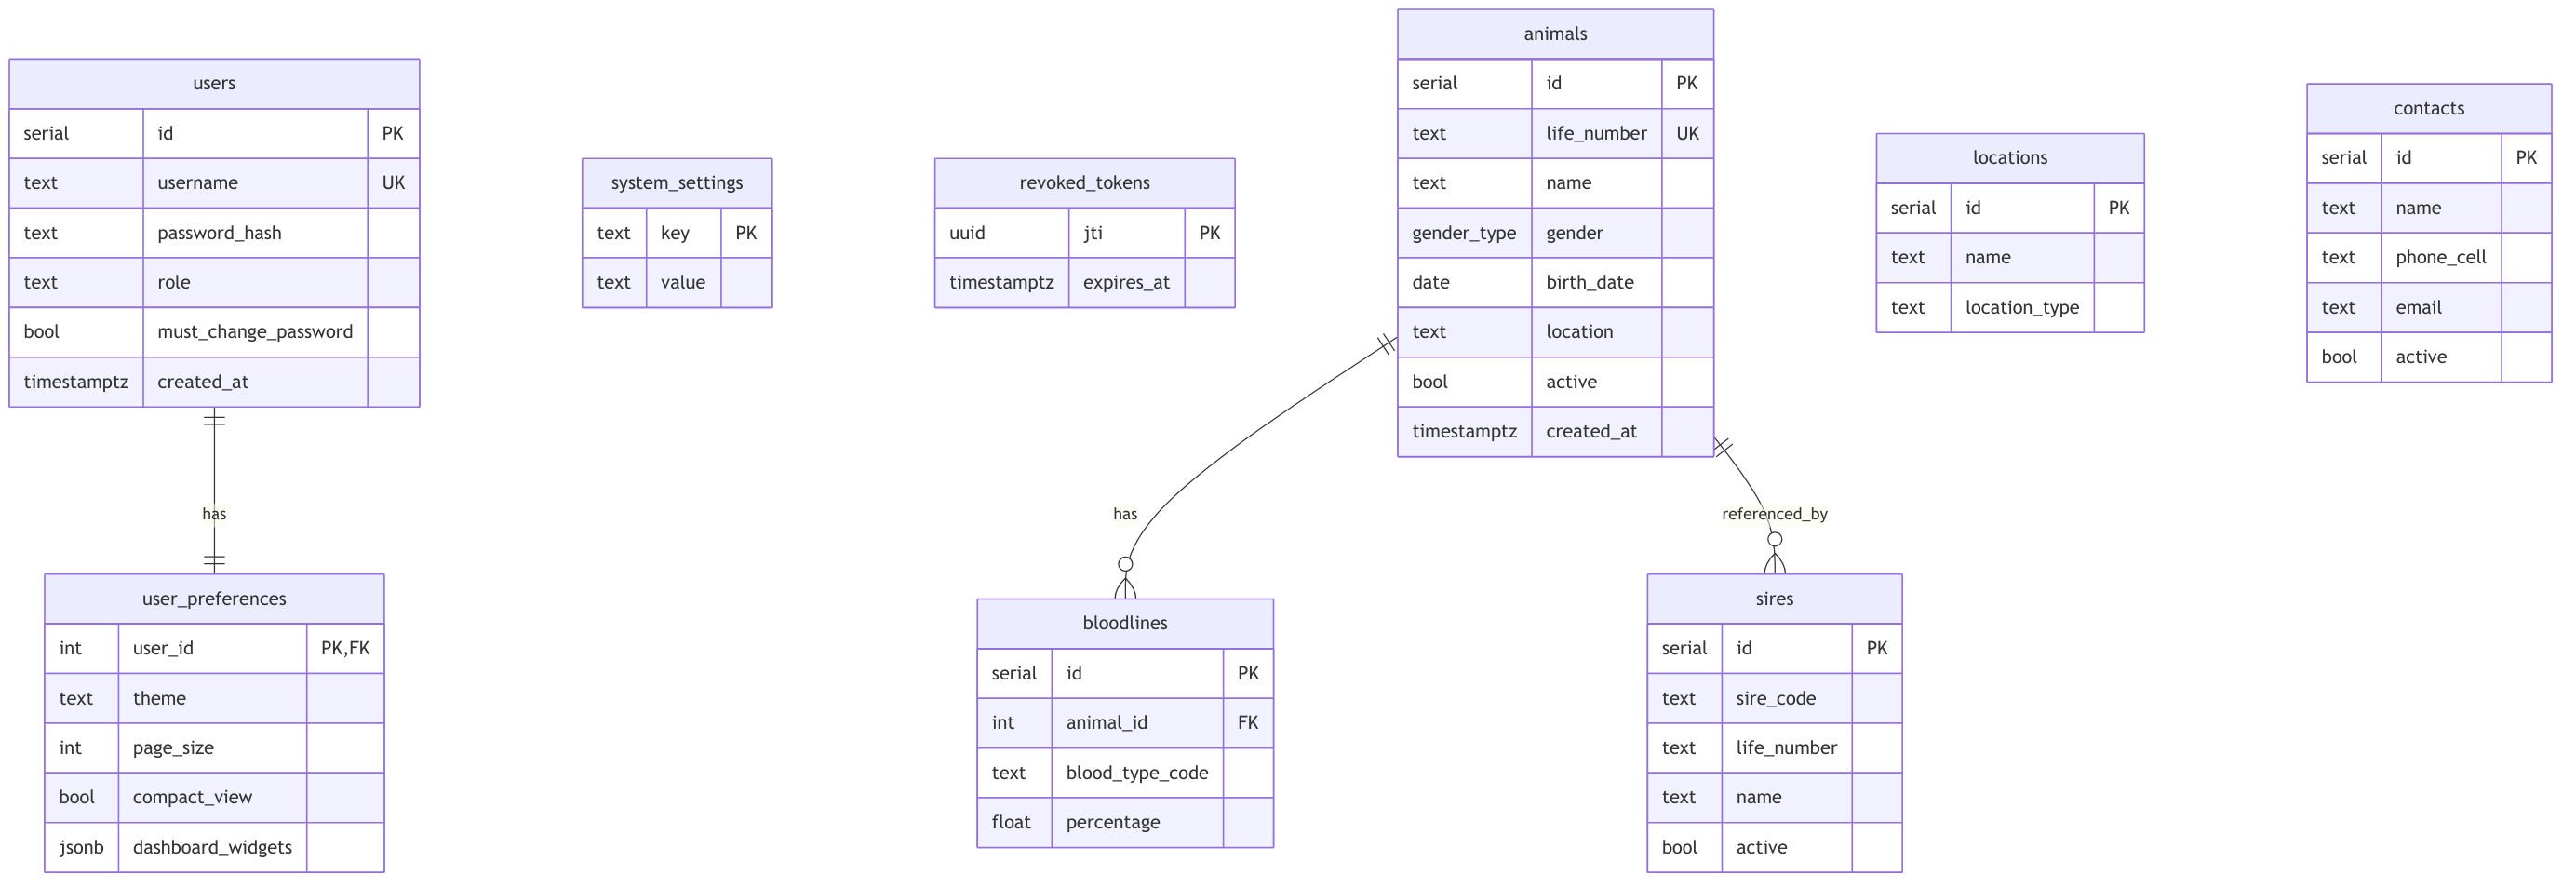
\includegraphics[width=0.95\textwidth,height=0.85\textheight,keepaspectratio]{db-core.png}
  \caption{ER-диаграмма: пользователи и реестр животных}
  \label{er-core}
\end{figure}

\textbf{Воспроизводство и выбраковка}

На рисунке~\ref{er-repro} представлены таблицы воспроизводства. Каждая таблица связана с животным через внешний ключ \texttt{animal\_id}. Таблица \texttt{calves} связана с \texttt{calvings} каскадным удалением. Таблица \texttt{culling\_events} используется как источник меток для ML-модели прогнозирования выбраковки.

\begin{figure}
  \centering
  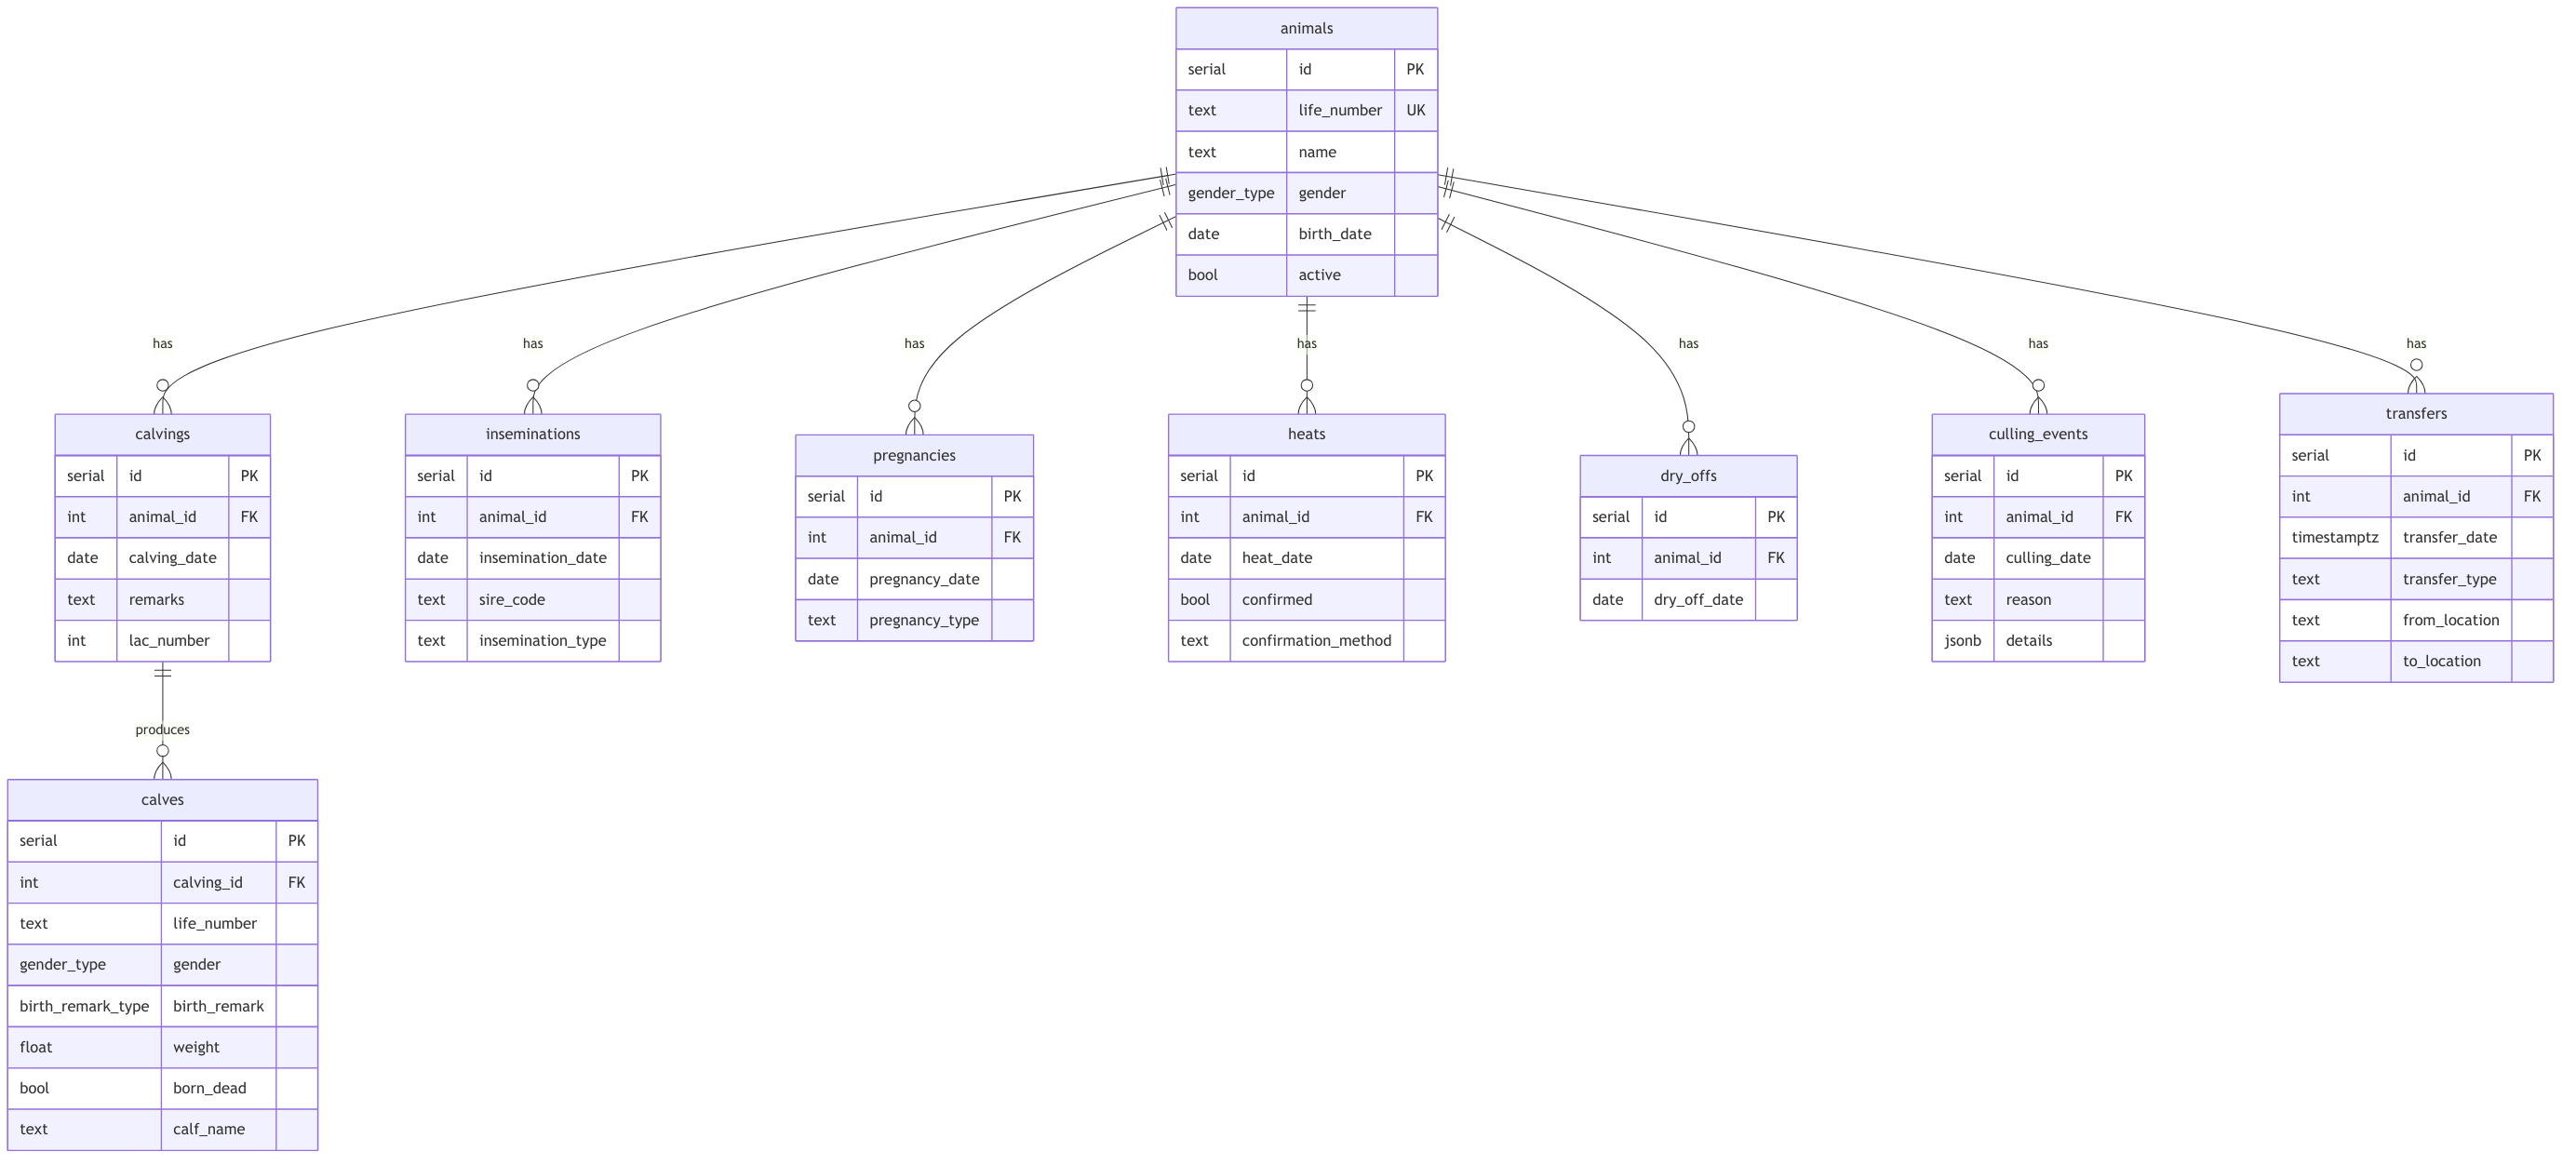
\includegraphics[width=0.95\textwidth,height=0.85\textheight,keepaspectratio]{db-repro.png}
  \caption{ER-диаграмма: воспроизводство и выбраковка}
  \label{er-repro}
\end{figure}

\textbf{Доение и молоко}

На рисунке~\ref{er-milk} представлены таблицы учёта надоев. Все таблицы, кроме \texttt{bulk\_tank\_tests}, привязаны к конкретному животному. Таблицы \texttt{milk\_day\_productions}, \texttt{milk\_visits}, \texttt{milk\_quality}, \texttt{milk\_visit\_quality} и \texttt{robot\_milk\_data} являются гипертаблицами TimescaleDB с партицировкой по 7 дней.

\begin{figure}
  \centering
  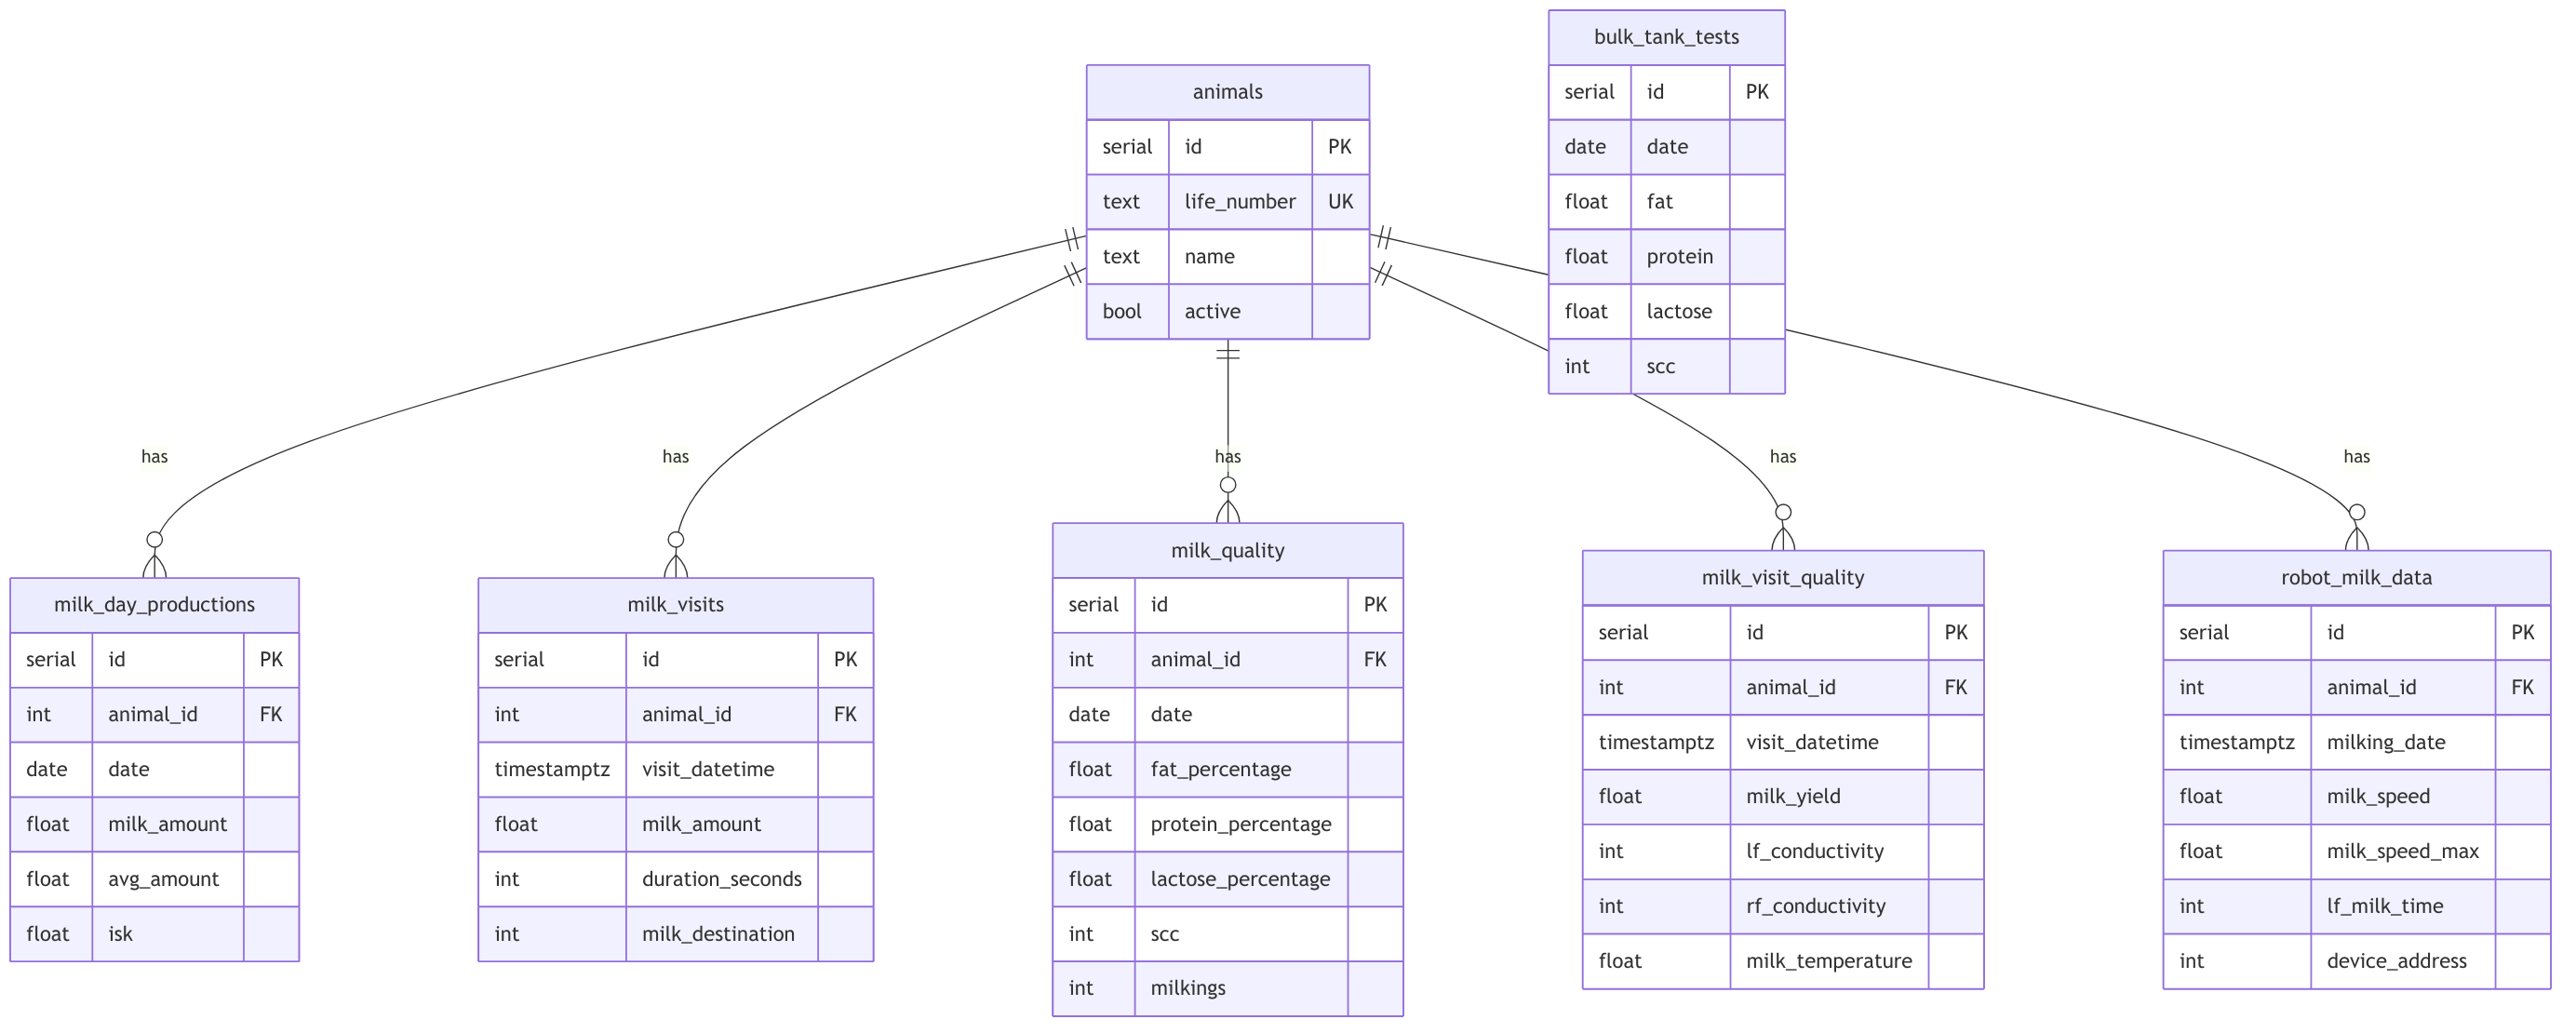
\includegraphics[width=0.95\textwidth,height=0.85\textheight,keepaspectratio]{db-milk.png}
  \caption{ER-диаграмма: доение и молоко}
  \label{er-milk}
\end{figure}

\textbf{Кормление, здоровье и активность}

На рисунке~\ref{er-feed} представлены таблицы кормления и мониторинга здоровья. Таблицы \texttt{feed\_day\_amounts}, \texttt{feed\_visits}, \texttt{activities} и \texttt{ruminations} являются гипертаблицами TimescaleDB. Таблица \texttt{vet\_records} содержит поля \texttt{diagnosis\_code} и \texttt{confirmed}, используемые как метки для ML-моделей.

\begin{figure}
  \centering
  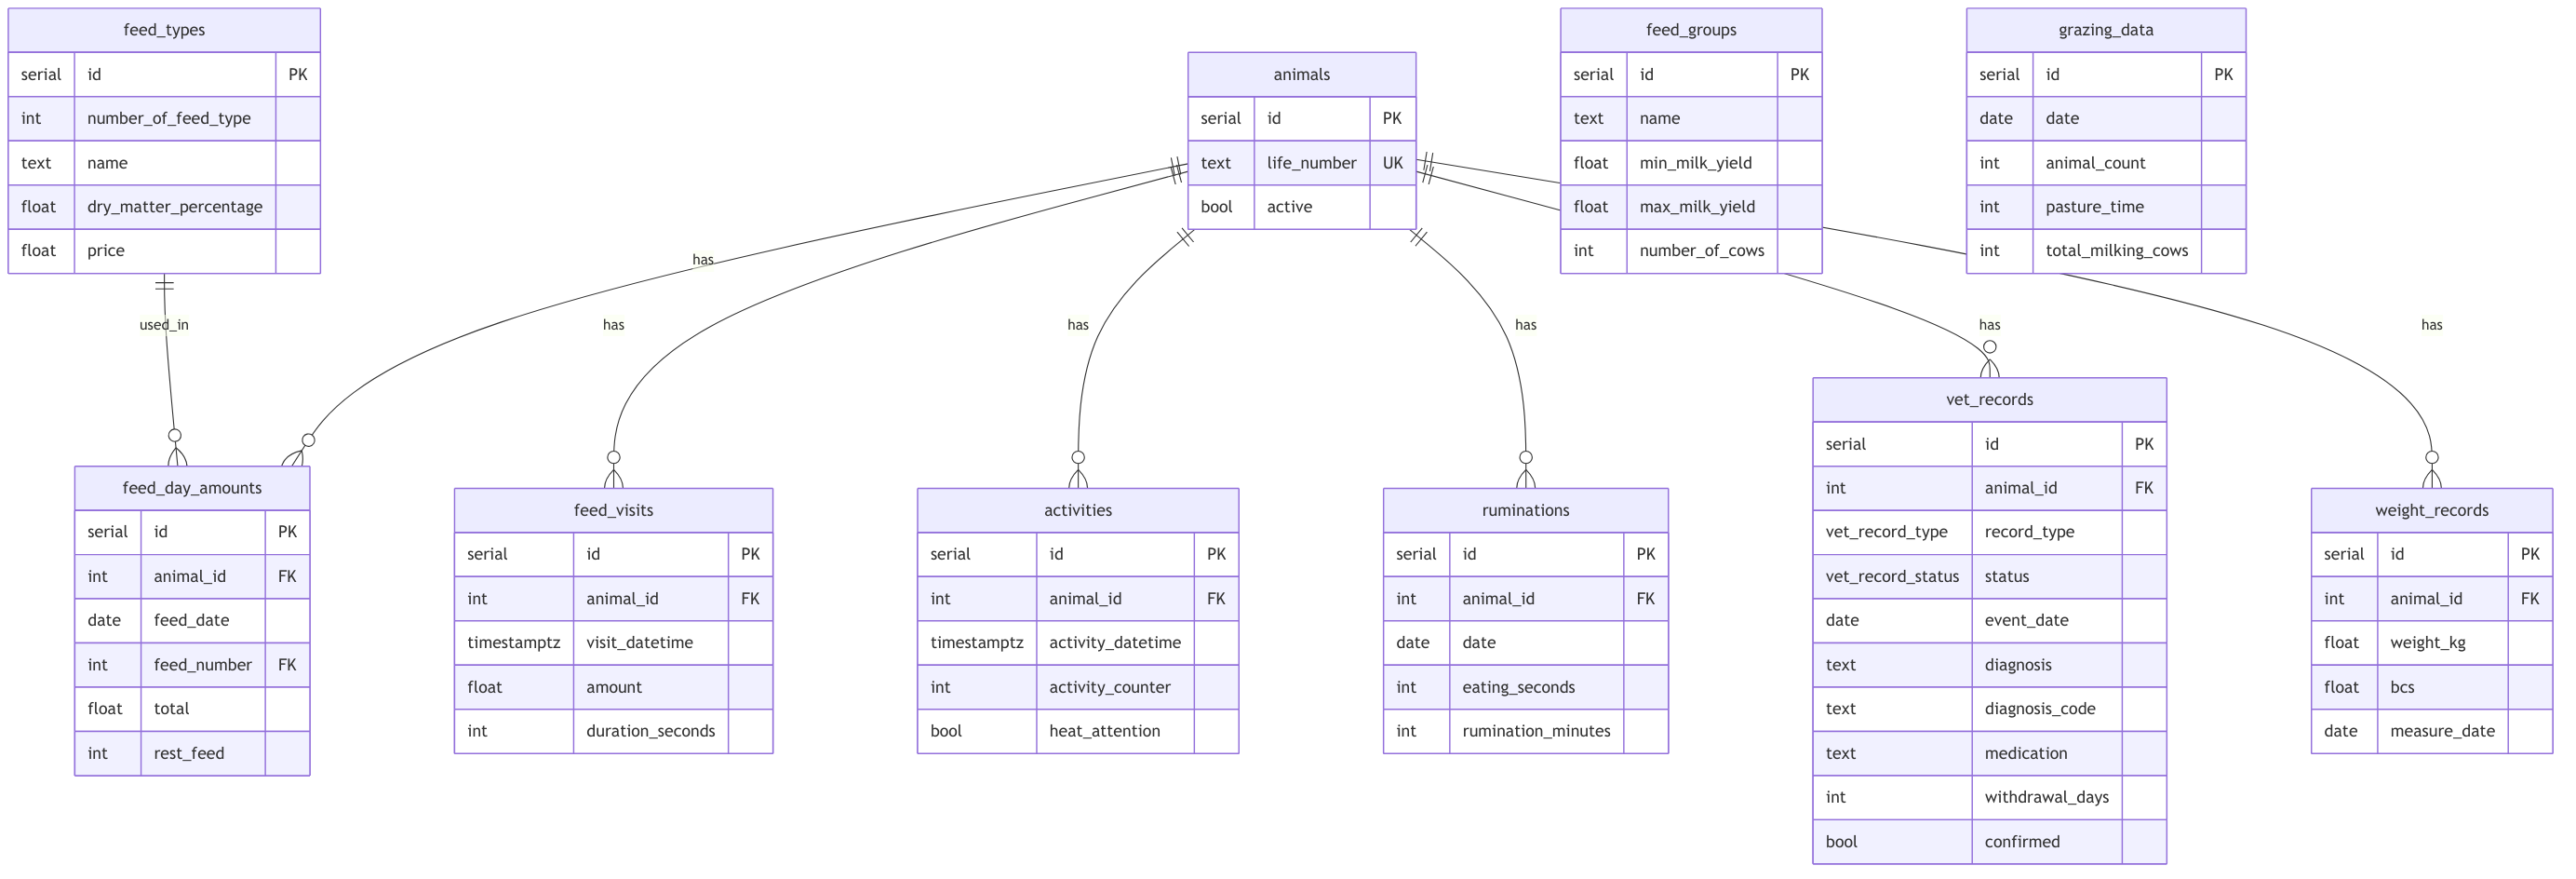
\includegraphics[width=0.95\textwidth,height=0.85\textheight,keepaspectratio]{db-feed-health.png}
  \caption{ER-диаграмма: кормление, здоровье и активность}
  \label{er-feed}
\end{figure}

\textbf{Оповещения и операции}

На рисунке~\ref{er-alerts} представлены таблицы оповещений, задач, аудита, финансов и учёта запасов. Оповещения создаются автоматически движком правил \texttt{alert\_engine} и доставляются через настраиваемые каналы уведомлений (браузер, Telegram).

\begin{figure}
  \centering
  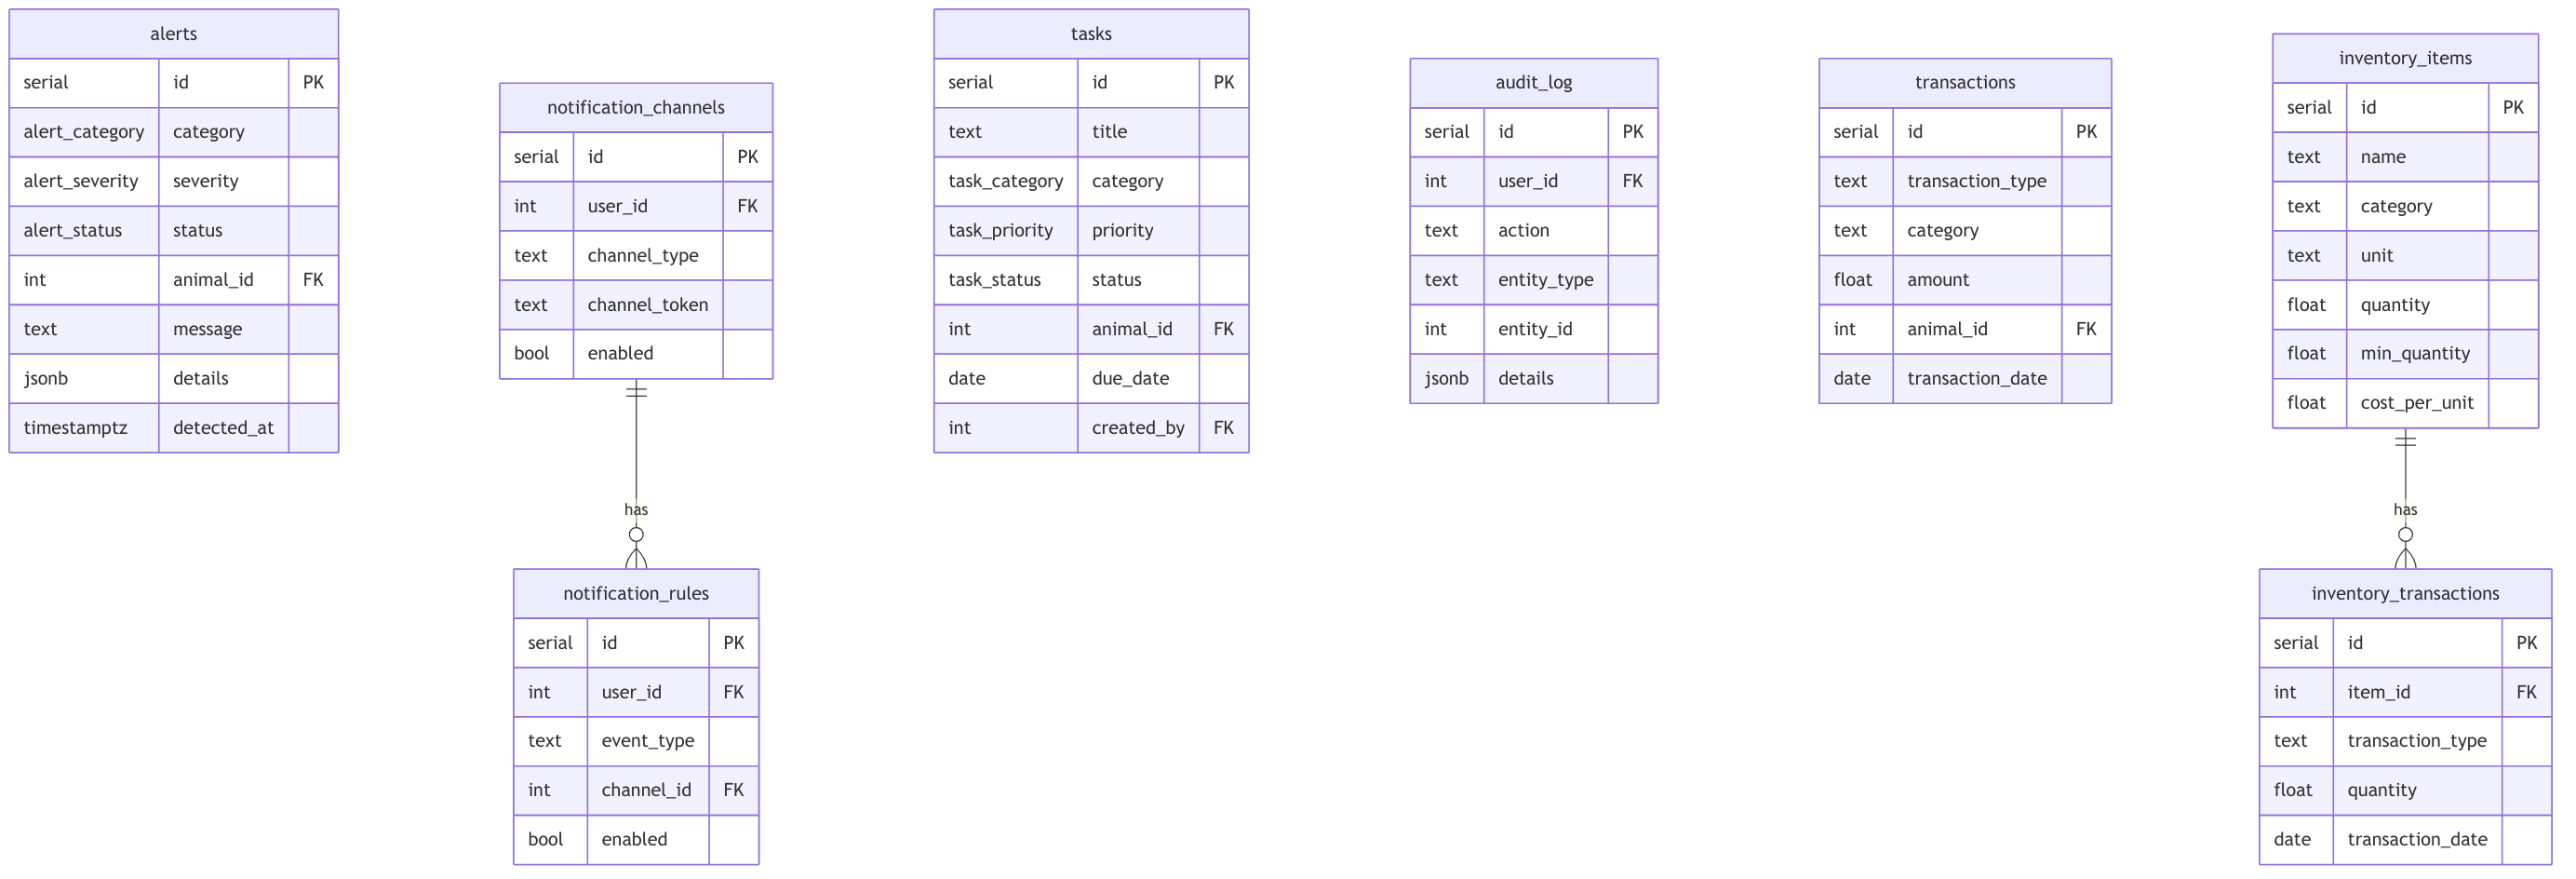
\includegraphics[width=0.95\textwidth,height=0.85\textheight,keepaspectratio]{db-alerts-ops.png}
  \caption{ER-диаграмма: оповещения и операции}
  \label{er-alerts}
\end{figure}

\textbf{Системные таблицы}

На рисунке~\ref{er-system} представлены системные таблицы: конфигурация интеграции с Lely с зашифрованными учётными данными, состояние синхронизации, зоны фермы и кэш погодных данных.

\begin{figure}
  \centering
  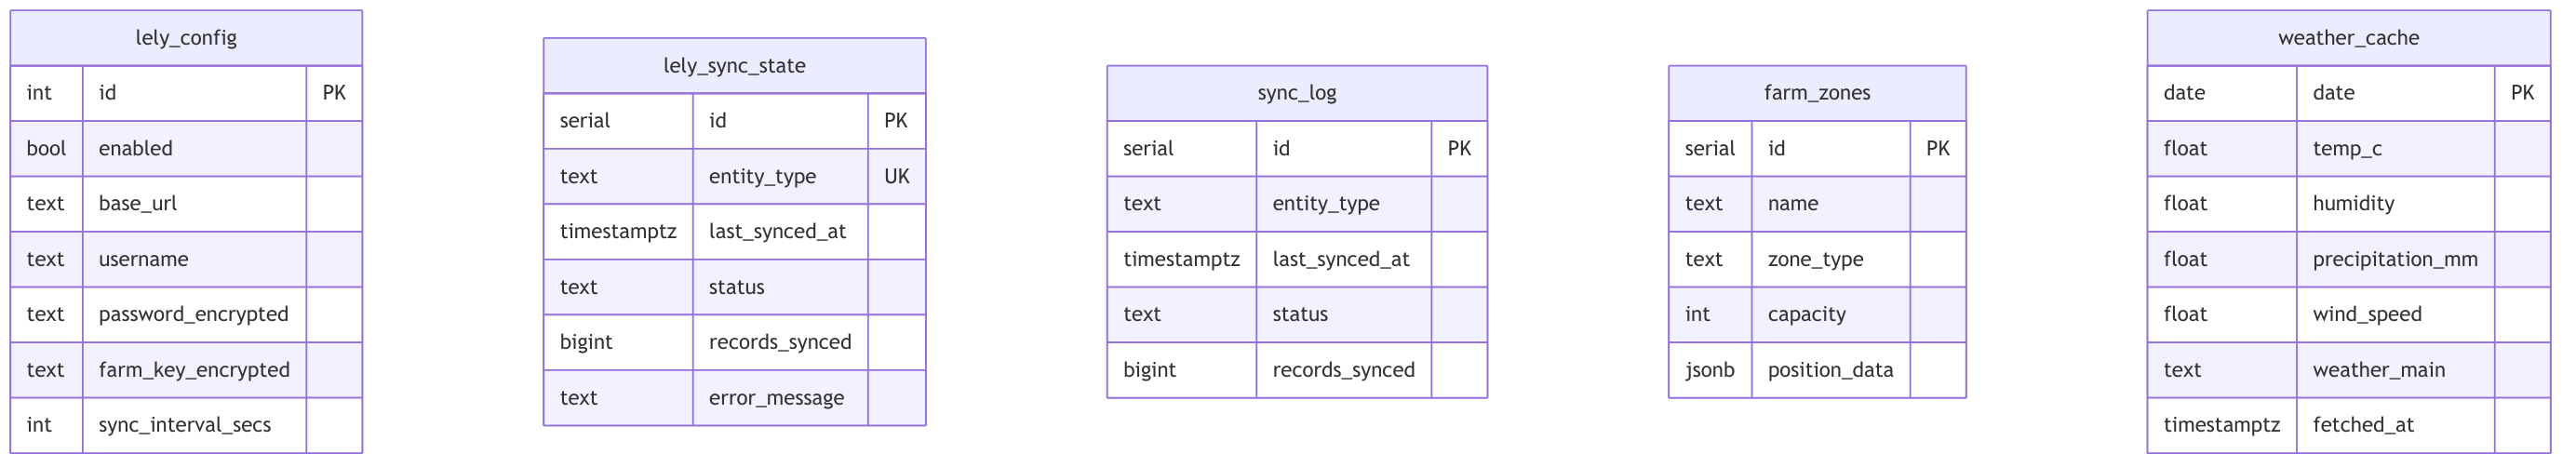
\includegraphics[width=0.95\textwidth,height=0.85\textheight,keepaspectratio]{db-system.png}
  \caption{ER-диаграмма: системные таблицы}
  \label{er-system}
\end{figure}

\appendixsection{Примеры API-запросов и ответов}
\label{app-api}

В данном приложении приведены примеры основных API-запросов и ответов информационной системы. Каждый рисунок содержит запрос и соответствующий ответ сервера.

\begin{figure}
  \begin{lstlisting}[basicstyle=\small\ttfamily]
POST /api/v1/auth/login
Content-Type: application/json

{
  "username": "admin",
  "password": "securepassword"
}
\end{lstlisting}
\vspace{0.5em}
\begin{lstlisting}[basicstyle=\small\ttfamily]
200 OK
Set-Cookie: token=eyJhbGci...; HttpOnly; SameSite=Strict
Set-Cookie: refresh_token=eyJhbGci...; HttpOnly; SameSite=Strict

{
  "user": {
    "username": "admin",
    "role": "admin",
    "must_change_password": false
  }
}
\end{lstlisting}
  \caption{Аутентификация: POST /api/v1/auth/login}
  \label{api-auth}
\end{figure}

\begin{figure}
  \begin{lstlisting}[basicstyle=\small\ttfamily]
GET /api/v1/animals?page=1&page_size=25&gender=female
Cookie: token=eyJhbGci...
\end{lstlisting}
\vspace{0.5em}
\begin{lstlisting}[basicstyle=\small\ttfamily]
200 OK
{
  "items": [
    {
      "id": 1,
      "life_number": "RU123456789",
      "name": "...",
      "gender": "female",
      "birth_date": "2020-03-15",
      "active": true
    }
  ],
  "total": 156,
  "page": 1,
  "page_size": 25
}
\end{lstlisting}
  \caption{Получение списка животных: GET /api/v1/animals}
  \label{api-animals}
\end{figure}

\begin{figure}
  \begin{lstlisting}[basicstyle=\small\ttfamily]
POST /api/v1/analytics/milk-trends
Content-Type: application/json

{
  "animal_id": 1,
  "days_ahead": 14
}
\end{lstlisting}
\vspace{0.5em}
\begin{lstlisting}[basicstyle=\small\ttfamily]
200 OK
{
  "animal_id": 1,
  "forecast": [
    {
      "date": "2026-04-21",
      "predicted_milk_kg": 28.5,
      "lower_bound": 25.1,
      "upper_bound": 31.9
    },
    {
      "date": "2026-04-22",
      "predicted_milk_kg": 28.2,
      "lower_bound": 24.8,
      "upper_bound": 31.6
    }
  ],
  "model": "holt_winters",
  "last_actual_date": "2026-04-20"
}
\end{lstlisting}
  \caption{Прогноз надоев: POST /api/v1/analytics/milk-trends}
  \label{api-forecast}
\end{figure}

\begin{figure}
  \begin{lstlisting}[basicstyle=\small\ttfamily]
POST /predict/mastitis
Content-Type: application/json
X-API-Key: <api_key>

{
  "animal_id": 1,
  "scc": 350000,
  "conductivity": 8.5,
  "fpr": 1.45,
  "milk_change_pct": -15.0,
  "dim": 45,
  "lactation": 2
}
\end{lstlisting}
\vspace{0.5em}
\begin{lstlisting}[basicstyle=\small\ttfamily]
200 OK
{
  "animal_id": 1,
  "risk_level": "high",
  "probability": 0.87,
  "contributing_factors": [
    {"factor": "scc_change", "importance": 0.35},
    {"factor": "conductivity", "importance": 0.25},
    {"factor": "milk_change", "importance": 0.20}
  ]
}
\end{lstlisting}
  \caption{Обнаружение мастита: POST /predict/mastitis}
  \label{api-mastitis}
\end{figure}

\begin{figure}
  \begin{lstlisting}[basicstyle=\small\ttfamily]
GET /api/v1/reports/export/R16/csv?date_from=2026-04-01
Cookie: token=eyJhbGci...
\end{lstlisting}
\vspace{0.5em}
\begin{lstlisting}[basicstyle=\small\ttfamily]
200 OK
Content-Type: text/csv
Content-Disposition: attachment; filename="R16_2026-04-20.csv"

date,total_milk_kg,avg_milk_kg,avg_fat_pct
2026-04-01,4350.0,29.0,3.85
2026-04-02,4280.5,28.5,3.82
\end{lstlisting}
  \caption{Экспорт отчёта в CSV: GET /api/v1/reports/export}
  \label{api-export}
\end{figure}

%\appendixsection{Листинги исходного кода}

В данном приложении приведены фрагменты исходного кода основных компонентов системы.

\subsubsection{Создание приложения и маршрутизация (Rust)}

Ниже приведён фрагмент файла \texttt{backend/src/lib.rs}, отвечающий за создание экземпляра приложения Axum с маршрутизацией и middleware.

\begin{lstlisting}[language=C,basicstyle=\small\ttfamily]
pub fn create_app(state: AppState) -> Router {
    let api_routes = Router::new()
        .nest("/auth",       handlers::auth::router())
        .nest("/animals",    handlers::animals::router())
        .nest("/milk",       handlers::milk::router())
        .nest("/reproduction",
                                handlers::reproduction::router())
        .nest("/feed",       handlers::feed::router())
        .nest("/fitness",    handlers::fitness::router())
        .nest("/reports",    handlers::reports::router())
        .nest("/analytics",  handlers::analytics::router())
        .nest("/settings",   handlers::settings::router())
        .nest("/lely",       handlers::lely::router());

    Router::new()
        .nest("/api/v1", api_routes)
        .layer(CsrfLayer)
        .layer(RateLimitLayer)
        .layer(MetricsLayer)
        .layer(CompressionLayer)
        .layer(CorsLayer)
        .with_state(state)
}
\end{lstlisting}

\subsubsection{Экстрактор авторизации (Rust)}

Ниже приведена реализация экстрактора \texttt{Claims}, извлекающего и проверяющего JWT-токен из запроса.

\begin{lstlisting}[language=C,basicstyle=\small\ttfamily]
pub struct Claims {
    pub sub: String,
    pub role: String,
    pub must_change_password: bool,
    pub jti: String,
    pub exp: i64,
}

#[async_trait]
impl<S: Send + Sync> FromRequestParts<S> for Claims {
    type Rejection = AppError;

    async fn from_request_parts(
        parts: &mut Parts,
        _state: &S,
    ) -> Result<Self, Self::Rejection> {
        let token = extract_token(parts)?;
        let claims = decode_jwt(&token)?;
        if claims.must_change_password {
            return Err(AppError::Forbidden);
        }
        check_revoked(&claims.jti).await?;
        Ok(claims)
    }
}
\end{lstlisting}

\subsubsection{Обучение модели XGBoost (Python)}

Ниже приведён фрагмент сервиса обучения модели прогнозирования надоев.

\begin{lstlisting}[language=Python,basicstyle=\small\ttfamily]
def train_milk_forecast(df: pd.DataFrame) -> dict:
    features = [
        "milk_7d_avg", "milk_14d_avg", "milk_30d_avg",
        "milk_7d_std", "milk_14d_std",
        "dim", "lactation_number", "fpr",
        "month", "day_of_week",
    ]
    X = df[features]
    y = df["milk_kg"]

    models = {}
    for q in [0.1, 0.5, 0.9]:
        model = xgb.XGBRegressor(
            objective="reg:quantileerror",
            quantile_alpha=q,
            n_estimators=200,
            max_depth=6,
            learning_rate=0.05,
            subsample=0.8,
            colsample_bytree=0.8,
        )
        model.fit(X, y)
        models[q] = model

    return models
\end{lstlisting}

\subsubsection{API-клиент (TypeScript)}

Ниже приведён фрагмент типизированного API-клиента на стороне frontend.

\begin{lstlisting}[language=Java,basicstyle=\small\ttfamily]
export const animalsApi = {
  list: (params: AnimalFilter) =>
    get<PaginatedResponse<Animal>>(
      "/animals?" + buildQuery(params)
    ),
  getById: (id: number) =>
    get<Animal>(`/animals/${id}`),
  create: (data: CreateAnimal) =>
    post<Animal>("/animals", data),
  update: (id: number, data: UpdateAnimal) =>
    put<Animal>(`/animals/${id}`, data),
  deactivate: (id: number) =>
    del(`/animals/${id}`),
  batchDeactivate: (ids: number[]) =>
    post("/animals/batch/deactivate", { ids }),
};
\end{lstlisting}

\end{document}
